\documentclass[twoside]{book}

% Packages required by doxygen
\usepackage{fixltx2e}
\usepackage{calc}
\usepackage{doxygen}
\usepackage[export]{adjustbox} % also loads graphicx
\usepackage{graphicx}
\usepackage[utf8]{inputenc}
\usepackage{makeidx}
\usepackage{multicol}
\usepackage{multirow}
\PassOptionsToPackage{warn}{textcomp}
\usepackage{textcomp}
\usepackage[nointegrals]{wasysym}
\usepackage[table]{xcolor}

% Font selection
\usepackage[T1]{fontenc}
\usepackage[scaled=.90]{helvet}
\usepackage{courier}
\usepackage{amssymb}
\usepackage{sectsty}
\renewcommand{\familydefault}{\sfdefault}
\allsectionsfont{%
  \fontseries{bc}\selectfont%
  \color{darkgray}%
}
\renewcommand{\DoxyLabelFont}{%
  \fontseries{bc}\selectfont%
  \color{darkgray}%
}
\newcommand{\+}{\discretionary{\mbox{\scriptsize$\hookleftarrow$}}{}{}}

% Page & text layout
\usepackage{geometry}
\geometry{%
  a4paper,%
  top=2.5cm,%
  bottom=2.5cm,%
  left=2.5cm,%
  right=2.5cm%
}
\tolerance=750
\hfuzz=15pt
\hbadness=750
\setlength{\emergencystretch}{15pt}
\setlength{\parindent}{0cm}
\setlength{\parskip}{3ex plus 2ex minus 2ex}
\makeatletter
\renewcommand{\paragraph}{%
  \@startsection{paragraph}{4}{0ex}{-1.0ex}{1.0ex}{%
    \normalfont\normalsize\bfseries\SS@parafont%
  }%
}
\renewcommand{\subparagraph}{%
  \@startsection{subparagraph}{5}{0ex}{-1.0ex}{1.0ex}{%
    \normalfont\normalsize\bfseries\SS@subparafont%
  }%
}
\makeatother

% Headers & footers
\usepackage{fancyhdr}
\pagestyle{fancyplain}
\fancyhead[LE]{\fancyplain{}{\bfseries\thepage}}
\fancyhead[CE]{\fancyplain{}{}}
\fancyhead[RE]{\fancyplain{}{\bfseries\leftmark}}
\fancyhead[LO]{\fancyplain{}{\bfseries\rightmark}}
\fancyhead[CO]{\fancyplain{}{}}
\fancyhead[RO]{\fancyplain{}{\bfseries\thepage}}
\fancyfoot[LE]{\fancyplain{}{}}
\fancyfoot[CE]{\fancyplain{}{}}
\fancyfoot[RE]{\fancyplain{}{\bfseries\scriptsize Generated by Doxygen }}
\fancyfoot[LO]{\fancyplain{}{\bfseries\scriptsize Generated by Doxygen }}
\fancyfoot[CO]{\fancyplain{}{}}
\fancyfoot[RO]{\fancyplain{}{}}
\renewcommand{\footrulewidth}{0.4pt}
\renewcommand{\chaptermark}[1]{%
  \markboth{#1}{}%
}
\renewcommand{\sectionmark}[1]{%
  \markright{\thesection\ #1}%
}

% Indices & bibliography
\usepackage{natbib}
\usepackage[titles]{tocloft}
\setcounter{tocdepth}{3}
\setcounter{secnumdepth}{5}
\makeindex

% Hyperlinks (required, but should be loaded last)
\usepackage{ifpdf}
\ifpdf
  \usepackage[pdftex,pagebackref=true]{hyperref}
\else
  \usepackage[ps2pdf,pagebackref=true]{hyperref}
\fi
\hypersetup{%
  colorlinks=true,%
  linkcolor=blue,%
  citecolor=blue,%
  unicode%
}

% Custom commands
\newcommand{\clearemptydoublepage}{%
  \newpage{\pagestyle{empty}\cleardoublepage}%
}

\usepackage{caption}
\captionsetup{labelsep=space,justification=centering,font={bf},singlelinecheck=off,skip=4pt,position=top}

%===== C O N T E N T S =====

\begin{document}

% Titlepage & ToC
\hypersetup{pageanchor=false,
             bookmarksnumbered=true,
             pdfencoding=unicode
            }
\pagenumbering{alph}
\begin{titlepage}
\vspace*{7cm}
\begin{center}%
{\Large Si7021\+\_\+\+E\+S\+P-\/\+I\+DF \\[1ex]\large 1.\+0 }\\
\vspace*{1cm}
{\large Generated by Doxygen 1.8.13}\\
\end{center}
\end{titlepage}
\clearemptydoublepage
\pagenumbering{roman}
\tableofcontents
\clearemptydoublepage
\pagenumbering{arabic}
\hypersetup{pageanchor=true}

%--- Begin generated contents ---
\chapter{R\+E\+A\+D\+ME}
\label{md_README}
\Hypertarget{md_README}
This is a library for communicating with S\+I7021 on E\+S\+P32 and E\+S\+P\+\_\+\+I\+DF framework

Copyright (C) 2019 Le Nguyen Hoang Nhan

This program is free software\+: you can redistribute it and/or modify it under the terms of the G\+NU General Public License as published by the Free Software Foundation, either version 3 of the License, or (at your option) any later version. This program is distributed in the hope that it will be useful, but W\+I\+T\+H\+O\+UT A\+NY W\+A\+R\+R\+A\+N\+TY; without even the implied warranty of M\+E\+R\+C\+H\+A\+N\+T\+A\+B\+I\+L\+I\+TY or F\+I\+T\+N\+E\+SS F\+OR A P\+A\+R\+T\+I\+C\+U\+L\+AR P\+U\+R\+P\+O\+SE. See the G\+NU General Public License for more details.

You should have received a copy of the G\+NU General Public License along with this program. If not, see \href{https://www.gnu.org/licenses/}{\tt https\+://www.\+gnu.\+org/licenses/}. 
\chapter{Module Index}
\section{Modules}
Here is a list of all modules\+:\begin{DoxyCompactList}
\item \contentsline{section}{S\+I7021 I2C Commands}{\pageref{group__SI7021__I2C__CMD}}{}
\item \contentsline{section}{S\+I7021 Return Value}{\pageref{group__SI7021__RT__VALUE}}{}
\item \contentsline{section}{S\+I7021 resolution in hex}{\pageref{group__SI7021__RES__HEX}}{}
\end{DoxyCompactList}

\chapter{Data Structure Index}
\section{Data Structures}
Here are the data structures with brief descriptions\+:\begin{DoxyCompactList}
\item\contentsline{section}{\hyperlink{structsi7021__config__t}{si7021\+\_\+config\+\_\+t} \\*S\+I7021 initialization parameter }{\pageref{structsi7021__config__t}}{}
\end{DoxyCompactList}

\chapter{File Index}
\section{File List}
Here is a list of all files with brief descriptions\+:\begin{DoxyCompactList}
\item\contentsline{section}{\hyperlink{si7021_8c}{si7021.\+c} \\*S\+I7021 Library for E\+S\+P-\/\+I\+DF framework main C file }{\pageref{si7021_8c}}{}
\item\contentsline{section}{include/\hyperlink{si7021_8h}{si7021.\+h} \\*S\+I7021 Library for E\+S\+P-\/\+I\+DF framework header file }{\pageref{si7021_8h}}{}
\end{DoxyCompactList}

\chapter{Module Documentation}
\hypertarget{group__SI7021__I2C__CMD}{}\section{S\+I7021 I2C Commands}
\label{group__SI7021__I2C__CMD}\index{S\+I7021 I2\+C Commands@{S\+I7021 I2\+C Commands}}
\subsection*{Macros}
\begin{DoxyCompactItemize}
\item 
\#define \hyperlink{group__SI7021__I2C__CMD_ga999d78aa56f7bd9ce04bb52e691d6753}{S\+I7021\+\_\+\+M\+E\+A\+S\+R\+H\+\_\+\+H\+O\+L\+D\+\_\+\+C\+MD}~0x\+E5
\item 
\#define \hyperlink{group__SI7021__I2C__CMD_ga7982df3514be8aa0cfef6e87e0aa48b0}{S\+I7021\+\_\+\+M\+E\+A\+S\+R\+H\+\_\+\+N\+O\+H\+O\+L\+D\+\_\+\+C\+MD}~0x\+F5
\item 
\#define \hyperlink{group__SI7021__I2C__CMD_ga2afcdc38468c893701a91bbf41c3e3d5}{S\+I7021\+\_\+\+M\+E\+A\+S\+T\+E\+M\+P\+\_\+\+H\+O\+L\+D\+\_\+\+C\+MD}~0x\+E3
\item 
\#define \hyperlink{group__SI7021__I2C__CMD_gad008920c3e715fc4c63032daca3bc5b0}{S\+I7021\+\_\+\+M\+E\+A\+S\+T\+E\+M\+P\+\_\+\+N\+O\+H\+O\+L\+D\+\_\+\+C\+MD}~0x\+F3
\item 
\#define \hyperlink{group__SI7021__I2C__CMD_gaf69388821d62e94cccd567f8861743a3}{S\+I7021\+\_\+\+R\+E\+A\+D\+P\+R\+E\+V\+T\+E\+M\+P\+\_\+\+C\+MD}~0x\+E0
\item 
\#define \hyperlink{group__SI7021__I2C__CMD_gaf46ed75ac39abc8aa85a2f08f6eaf2fb}{S\+I7021\+\_\+\+R\+E\+S\+E\+T\+\_\+\+C\+MD}~0x\+FE
\item 
\#define \hyperlink{group__SI7021__I2C__CMD_gaec66f83a736566c680c195cad9f7cb7c}{S\+I7021\+\_\+\+W\+R\+I\+T\+E\+R\+H\+T\+\_\+\+R\+E\+G\+\_\+\+C\+MD}~0x\+E6
\item 
\#define \hyperlink{group__SI7021__I2C__CMD_ga39482cdbef1a96514a58d25c30cab869}{S\+I7021\+\_\+\+R\+E\+A\+D\+R\+H\+T\+\_\+\+R\+E\+G\+\_\+\+C\+MD}~0x\+E7
\item 
\#define \hyperlink{group__SI7021__I2C__CMD_gaf62a1fb7fe727aa31f52de3ce616e3a4}{S\+I7021\+\_\+\+W\+R\+I\+T\+E\+H\+E\+A\+T\+E\+R\+\_\+\+R\+E\+G\+\_\+\+C\+MD}~0x51
\item 
\#define \hyperlink{group__SI7021__I2C__CMD_ga3b1583b7a4599056347a0f8fea5349fa}{S\+I7021\+\_\+\+R\+E\+A\+D\+H\+E\+A\+T\+E\+R\+\_\+\+R\+E\+G\+\_\+\+C\+MD}~0x11
\item 
\#define \hyperlink{group__SI7021__I2C__CMD_ga4b71181e51a490ca8626758a80a0d14c}{S\+I7021\+\_\+\+I\+D1\+\_\+\+C\+MD}~0x\+F\+A0F
\item 
\#define \hyperlink{group__SI7021__I2C__CMD_ga65ab7ac27fe593eb11f4b0c4c9a16319}{S\+I7021\+\_\+\+I\+D2\+\_\+\+C\+MD}~0x\+F\+C\+C9
\item 
\#define \hyperlink{group__SI7021__I2C__CMD_ga2e429d79e5cca3c05d883b5509a88963}{S\+I7021\+\_\+\+F\+I\+R\+M\+V\+E\+R\+S\+\_\+\+C\+MD}~0x84\+B8
\item 
\#define \hyperlink{group__SI7021__I2C__CMD_ga6d880c26eb3b8bff87e47ee43dd5e8a4}{S\+I7021\+\_\+\+S\+O\+F\+T\+\_\+\+R\+E\+S\+E\+T\+\_\+\+C\+MD}~0x\+FE
\end{DoxyCompactItemize}


\subsection{Detailed Description}


\subsection{Macro Definition Documentation}
\mbox{\Hypertarget{group__SI7021__I2C__CMD_ga2e429d79e5cca3c05d883b5509a88963}\label{group__SI7021__I2C__CMD_ga2e429d79e5cca3c05d883b5509a88963}} 
\index{S\+I7021 I2\+C Commands@{S\+I7021 I2\+C Commands}!S\+I7021\+\_\+\+F\+I\+R\+M\+V\+E\+R\+S\+\_\+\+C\+MD@{S\+I7021\+\_\+\+F\+I\+R\+M\+V\+E\+R\+S\+\_\+\+C\+MD}}
\index{S\+I7021\+\_\+\+F\+I\+R\+M\+V\+E\+R\+S\+\_\+\+C\+MD@{S\+I7021\+\_\+\+F\+I\+R\+M\+V\+E\+R\+S\+\_\+\+C\+MD}!S\+I7021 I2\+C Commands@{S\+I7021 I2\+C Commands}}
\subsubsection{\texorpdfstring{S\+I7021\+\_\+\+F\+I\+R\+M\+V\+E\+R\+S\+\_\+\+C\+MD}{SI7021\_FIRMVERS\_CMD}}
{\footnotesize\ttfamily \#define S\+I7021\+\_\+\+F\+I\+R\+M\+V\+E\+R\+S\+\_\+\+C\+MD~0x84\+B8}

I2C command for reading firmware revision 

Definition at line 60 of file si7021.\+h.



Referenced by si7021\+\_\+read\+\_\+firmware\+\_\+rev().

\mbox{\Hypertarget{group__SI7021__I2C__CMD_ga4b71181e51a490ca8626758a80a0d14c}\label{group__SI7021__I2C__CMD_ga4b71181e51a490ca8626758a80a0d14c}} 
\index{S\+I7021 I2\+C Commands@{S\+I7021 I2\+C Commands}!S\+I7021\+\_\+\+I\+D1\+\_\+\+C\+MD@{S\+I7021\+\_\+\+I\+D1\+\_\+\+C\+MD}}
\index{S\+I7021\+\_\+\+I\+D1\+\_\+\+C\+MD@{S\+I7021\+\_\+\+I\+D1\+\_\+\+C\+MD}!S\+I7021 I2\+C Commands@{S\+I7021 I2\+C Commands}}
\subsubsection{\texorpdfstring{S\+I7021\+\_\+\+I\+D1\+\_\+\+C\+MD}{SI7021\_ID1\_CMD}}
{\footnotesize\ttfamily \#define S\+I7021\+\_\+\+I\+D1\+\_\+\+C\+MD~0x\+F\+A0F}

I2C command for reading 1st byte of electronic ID 

Definition at line 58 of file si7021.\+h.



Referenced by get\+\_\+electronic\+\_\+id().

\mbox{\Hypertarget{group__SI7021__I2C__CMD_ga65ab7ac27fe593eb11f4b0c4c9a16319}\label{group__SI7021__I2C__CMD_ga65ab7ac27fe593eb11f4b0c4c9a16319}} 
\index{S\+I7021 I2\+C Commands@{S\+I7021 I2\+C Commands}!S\+I7021\+\_\+\+I\+D2\+\_\+\+C\+MD@{S\+I7021\+\_\+\+I\+D2\+\_\+\+C\+MD}}
\index{S\+I7021\+\_\+\+I\+D2\+\_\+\+C\+MD@{S\+I7021\+\_\+\+I\+D2\+\_\+\+C\+MD}!S\+I7021 I2\+C Commands@{S\+I7021 I2\+C Commands}}
\subsubsection{\texorpdfstring{S\+I7021\+\_\+\+I\+D2\+\_\+\+C\+MD}{SI7021\_ID2\_CMD}}
{\footnotesize\ttfamily \#define S\+I7021\+\_\+\+I\+D2\+\_\+\+C\+MD~0x\+F\+C\+C9}

I2C command for reading 2nd byte of electronic ID 

Definition at line 59 of file si7021.\+h.



Referenced by get\+\_\+electronic\+\_\+id().

\mbox{\Hypertarget{group__SI7021__I2C__CMD_ga999d78aa56f7bd9ce04bb52e691d6753}\label{group__SI7021__I2C__CMD_ga999d78aa56f7bd9ce04bb52e691d6753}} 
\index{S\+I7021 I2\+C Commands@{S\+I7021 I2\+C Commands}!S\+I7021\+\_\+\+M\+E\+A\+S\+R\+H\+\_\+\+H\+O\+L\+D\+\_\+\+C\+MD@{S\+I7021\+\_\+\+M\+E\+A\+S\+R\+H\+\_\+\+H\+O\+L\+D\+\_\+\+C\+MD}}
\index{S\+I7021\+\_\+\+M\+E\+A\+S\+R\+H\+\_\+\+H\+O\+L\+D\+\_\+\+C\+MD@{S\+I7021\+\_\+\+M\+E\+A\+S\+R\+H\+\_\+\+H\+O\+L\+D\+\_\+\+C\+MD}!S\+I7021 I2\+C Commands@{S\+I7021 I2\+C Commands}}
\subsubsection{\texorpdfstring{S\+I7021\+\_\+\+M\+E\+A\+S\+R\+H\+\_\+\+H\+O\+L\+D\+\_\+\+C\+MD}{SI7021\_MEASRH\_HOLD\_CMD}}
{\footnotesize\ttfamily \#define S\+I7021\+\_\+\+M\+E\+A\+S\+R\+H\+\_\+\+H\+O\+L\+D\+\_\+\+C\+MD~0x\+E5}

I2C command for RH measuring, hold master mode 

Definition at line 48 of file si7021.\+h.

\mbox{\Hypertarget{group__SI7021__I2C__CMD_ga7982df3514be8aa0cfef6e87e0aa48b0}\label{group__SI7021__I2C__CMD_ga7982df3514be8aa0cfef6e87e0aa48b0}} 
\index{S\+I7021 I2\+C Commands@{S\+I7021 I2\+C Commands}!S\+I7021\+\_\+\+M\+E\+A\+S\+R\+H\+\_\+\+N\+O\+H\+O\+L\+D\+\_\+\+C\+MD@{S\+I7021\+\_\+\+M\+E\+A\+S\+R\+H\+\_\+\+N\+O\+H\+O\+L\+D\+\_\+\+C\+MD}}
\index{S\+I7021\+\_\+\+M\+E\+A\+S\+R\+H\+\_\+\+N\+O\+H\+O\+L\+D\+\_\+\+C\+MD@{S\+I7021\+\_\+\+M\+E\+A\+S\+R\+H\+\_\+\+N\+O\+H\+O\+L\+D\+\_\+\+C\+MD}!S\+I7021 I2\+C Commands@{S\+I7021 I2\+C Commands}}
\subsubsection{\texorpdfstring{S\+I7021\+\_\+\+M\+E\+A\+S\+R\+H\+\_\+\+N\+O\+H\+O\+L\+D\+\_\+\+C\+MD}{SI7021\_MEASRH\_NOHOLD\_CMD}}
{\footnotesize\ttfamily \#define S\+I7021\+\_\+\+M\+E\+A\+S\+R\+H\+\_\+\+N\+O\+H\+O\+L\+D\+\_\+\+C\+MD~0x\+F5}

I2C command for RH measuring, no hold master mode 

Definition at line 49 of file si7021.\+h.



Referenced by si7021\+\_\+read\+\_\+humidity().

\mbox{\Hypertarget{group__SI7021__I2C__CMD_ga2afcdc38468c893701a91bbf41c3e3d5}\label{group__SI7021__I2C__CMD_ga2afcdc38468c893701a91bbf41c3e3d5}} 
\index{S\+I7021 I2\+C Commands@{S\+I7021 I2\+C Commands}!S\+I7021\+\_\+\+M\+E\+A\+S\+T\+E\+M\+P\+\_\+\+H\+O\+L\+D\+\_\+\+C\+MD@{S\+I7021\+\_\+\+M\+E\+A\+S\+T\+E\+M\+P\+\_\+\+H\+O\+L\+D\+\_\+\+C\+MD}}
\index{S\+I7021\+\_\+\+M\+E\+A\+S\+T\+E\+M\+P\+\_\+\+H\+O\+L\+D\+\_\+\+C\+MD@{S\+I7021\+\_\+\+M\+E\+A\+S\+T\+E\+M\+P\+\_\+\+H\+O\+L\+D\+\_\+\+C\+MD}!S\+I7021 I2\+C Commands@{S\+I7021 I2\+C Commands}}
\subsubsection{\texorpdfstring{S\+I7021\+\_\+\+M\+E\+A\+S\+T\+E\+M\+P\+\_\+\+H\+O\+L\+D\+\_\+\+C\+MD}{SI7021\_MEASTEMP\_HOLD\_CMD}}
{\footnotesize\ttfamily \#define S\+I7021\+\_\+\+M\+E\+A\+S\+T\+E\+M\+P\+\_\+\+H\+O\+L\+D\+\_\+\+C\+MD~0x\+E3}

I2C command for Temperature measuring, hold master mode 

Definition at line 50 of file si7021.\+h.

\mbox{\Hypertarget{group__SI7021__I2C__CMD_gad008920c3e715fc4c63032daca3bc5b0}\label{group__SI7021__I2C__CMD_gad008920c3e715fc4c63032daca3bc5b0}} 
\index{S\+I7021 I2\+C Commands@{S\+I7021 I2\+C Commands}!S\+I7021\+\_\+\+M\+E\+A\+S\+T\+E\+M\+P\+\_\+\+N\+O\+H\+O\+L\+D\+\_\+\+C\+MD@{S\+I7021\+\_\+\+M\+E\+A\+S\+T\+E\+M\+P\+\_\+\+N\+O\+H\+O\+L\+D\+\_\+\+C\+MD}}
\index{S\+I7021\+\_\+\+M\+E\+A\+S\+T\+E\+M\+P\+\_\+\+N\+O\+H\+O\+L\+D\+\_\+\+C\+MD@{S\+I7021\+\_\+\+M\+E\+A\+S\+T\+E\+M\+P\+\_\+\+N\+O\+H\+O\+L\+D\+\_\+\+C\+MD}!S\+I7021 I2\+C Commands@{S\+I7021 I2\+C Commands}}
\subsubsection{\texorpdfstring{S\+I7021\+\_\+\+M\+E\+A\+S\+T\+E\+M\+P\+\_\+\+N\+O\+H\+O\+L\+D\+\_\+\+C\+MD}{SI7021\_MEASTEMP\_NOHOLD\_CMD}}
{\footnotesize\ttfamily \#define S\+I7021\+\_\+\+M\+E\+A\+S\+T\+E\+M\+P\+\_\+\+N\+O\+H\+O\+L\+D\+\_\+\+C\+MD~0x\+F3}

I2C command for Temperature measuring, no hold master mode 

Definition at line 51 of file si7021.\+h.



Referenced by si7021\+\_\+read\+\_\+temperature().

\mbox{\Hypertarget{group__SI7021__I2C__CMD_ga3b1583b7a4599056347a0f8fea5349fa}\label{group__SI7021__I2C__CMD_ga3b1583b7a4599056347a0f8fea5349fa}} 
\index{S\+I7021 I2\+C Commands@{S\+I7021 I2\+C Commands}!S\+I7021\+\_\+\+R\+E\+A\+D\+H\+E\+A\+T\+E\+R\+\_\+\+R\+E\+G\+\_\+\+C\+MD@{S\+I7021\+\_\+\+R\+E\+A\+D\+H\+E\+A\+T\+E\+R\+\_\+\+R\+E\+G\+\_\+\+C\+MD}}
\index{S\+I7021\+\_\+\+R\+E\+A\+D\+H\+E\+A\+T\+E\+R\+\_\+\+R\+E\+G\+\_\+\+C\+MD@{S\+I7021\+\_\+\+R\+E\+A\+D\+H\+E\+A\+T\+E\+R\+\_\+\+R\+E\+G\+\_\+\+C\+MD}!S\+I7021 I2\+C Commands@{S\+I7021 I2\+C Commands}}
\subsubsection{\texorpdfstring{S\+I7021\+\_\+\+R\+E\+A\+D\+H\+E\+A\+T\+E\+R\+\_\+\+R\+E\+G\+\_\+\+C\+MD}{SI7021\_READHEATER\_REG\_CMD}}
{\footnotesize\ttfamily \#define S\+I7021\+\_\+\+R\+E\+A\+D\+H\+E\+A\+T\+E\+R\+\_\+\+R\+E\+G\+\_\+\+C\+MD~0x11}

I2C command for reading heater register 

Definition at line 57 of file si7021.\+h.



Referenced by si7021\+\_\+get\+\_\+heater\+\_\+register().

\mbox{\Hypertarget{group__SI7021__I2C__CMD_gaf69388821d62e94cccd567f8861743a3}\label{group__SI7021__I2C__CMD_gaf69388821d62e94cccd567f8861743a3}} 
\index{S\+I7021 I2\+C Commands@{S\+I7021 I2\+C Commands}!S\+I7021\+\_\+\+R\+E\+A\+D\+P\+R\+E\+V\+T\+E\+M\+P\+\_\+\+C\+MD@{S\+I7021\+\_\+\+R\+E\+A\+D\+P\+R\+E\+V\+T\+E\+M\+P\+\_\+\+C\+MD}}
\index{S\+I7021\+\_\+\+R\+E\+A\+D\+P\+R\+E\+V\+T\+E\+M\+P\+\_\+\+C\+MD@{S\+I7021\+\_\+\+R\+E\+A\+D\+P\+R\+E\+V\+T\+E\+M\+P\+\_\+\+C\+MD}!S\+I7021 I2\+C Commands@{S\+I7021 I2\+C Commands}}
\subsubsection{\texorpdfstring{S\+I7021\+\_\+\+R\+E\+A\+D\+P\+R\+E\+V\+T\+E\+M\+P\+\_\+\+C\+MD}{SI7021\_READPREVTEMP\_CMD}}
{\footnotesize\ttfamily \#define S\+I7021\+\_\+\+R\+E\+A\+D\+P\+R\+E\+V\+T\+E\+M\+P\+\_\+\+C\+MD~0x\+E0}

I2C command for reading previously measured temperature 

Definition at line 52 of file si7021.\+h.

\mbox{\Hypertarget{group__SI7021__I2C__CMD_ga39482cdbef1a96514a58d25c30cab869}\label{group__SI7021__I2C__CMD_ga39482cdbef1a96514a58d25c30cab869}} 
\index{S\+I7021 I2\+C Commands@{S\+I7021 I2\+C Commands}!S\+I7021\+\_\+\+R\+E\+A\+D\+R\+H\+T\+\_\+\+R\+E\+G\+\_\+\+C\+MD@{S\+I7021\+\_\+\+R\+E\+A\+D\+R\+H\+T\+\_\+\+R\+E\+G\+\_\+\+C\+MD}}
\index{S\+I7021\+\_\+\+R\+E\+A\+D\+R\+H\+T\+\_\+\+R\+E\+G\+\_\+\+C\+MD@{S\+I7021\+\_\+\+R\+E\+A\+D\+R\+H\+T\+\_\+\+R\+E\+G\+\_\+\+C\+MD}!S\+I7021 I2\+C Commands@{S\+I7021 I2\+C Commands}}
\subsubsection{\texorpdfstring{S\+I7021\+\_\+\+R\+E\+A\+D\+R\+H\+T\+\_\+\+R\+E\+G\+\_\+\+C\+MD}{SI7021\_READRHT\_REG\_CMD}}
{\footnotesize\ttfamily \#define S\+I7021\+\_\+\+R\+E\+A\+D\+R\+H\+T\+\_\+\+R\+E\+G\+\_\+\+C\+MD~0x\+E7}

I2C command for reading R\+H/T user register 1 

Definition at line 55 of file si7021.\+h.



Referenced by \+\_\+\+\_\+si7021\+\_\+read\+\_\+user\+\_\+register().

\mbox{\Hypertarget{group__SI7021__I2C__CMD_gaf46ed75ac39abc8aa85a2f08f6eaf2fb}\label{group__SI7021__I2C__CMD_gaf46ed75ac39abc8aa85a2f08f6eaf2fb}} 
\index{S\+I7021 I2\+C Commands@{S\+I7021 I2\+C Commands}!S\+I7021\+\_\+\+R\+E\+S\+E\+T\+\_\+\+C\+MD@{S\+I7021\+\_\+\+R\+E\+S\+E\+T\+\_\+\+C\+MD}}
\index{S\+I7021\+\_\+\+R\+E\+S\+E\+T\+\_\+\+C\+MD@{S\+I7021\+\_\+\+R\+E\+S\+E\+T\+\_\+\+C\+MD}!S\+I7021 I2\+C Commands@{S\+I7021 I2\+C Commands}}
\subsubsection{\texorpdfstring{S\+I7021\+\_\+\+R\+E\+S\+E\+T\+\_\+\+C\+MD}{SI7021\_RESET\_CMD}}
{\footnotesize\ttfamily \#define S\+I7021\+\_\+\+R\+E\+S\+E\+T\+\_\+\+C\+MD~0x\+FE}

I2C command for reseting sensors 

Definition at line 53 of file si7021.\+h.

\mbox{\Hypertarget{group__SI7021__I2C__CMD_ga6d880c26eb3b8bff87e47ee43dd5e8a4}\label{group__SI7021__I2C__CMD_ga6d880c26eb3b8bff87e47ee43dd5e8a4}} 
\index{S\+I7021 I2\+C Commands@{S\+I7021 I2\+C Commands}!S\+I7021\+\_\+\+S\+O\+F\+T\+\_\+\+R\+E\+S\+E\+T\+\_\+\+C\+MD@{S\+I7021\+\_\+\+S\+O\+F\+T\+\_\+\+R\+E\+S\+E\+T\+\_\+\+C\+MD}}
\index{S\+I7021\+\_\+\+S\+O\+F\+T\+\_\+\+R\+E\+S\+E\+T\+\_\+\+C\+MD@{S\+I7021\+\_\+\+S\+O\+F\+T\+\_\+\+R\+E\+S\+E\+T\+\_\+\+C\+MD}!S\+I7021 I2\+C Commands@{S\+I7021 I2\+C Commands}}
\subsubsection{\texorpdfstring{S\+I7021\+\_\+\+S\+O\+F\+T\+\_\+\+R\+E\+S\+E\+T\+\_\+\+C\+MD}{SI7021\_SOFT\_RESET\_CMD}}
{\footnotesize\ttfamily \#define S\+I7021\+\_\+\+S\+O\+F\+T\+\_\+\+R\+E\+S\+E\+T\+\_\+\+C\+MD~0x\+FE}

I2C command for soft reseting sensors 

Definition at line 61 of file si7021.\+h.



Referenced by si7021\+\_\+soft\+\_\+reset().

\mbox{\Hypertarget{group__SI7021__I2C__CMD_gaf62a1fb7fe727aa31f52de3ce616e3a4}\label{group__SI7021__I2C__CMD_gaf62a1fb7fe727aa31f52de3ce616e3a4}} 
\index{S\+I7021 I2\+C Commands@{S\+I7021 I2\+C Commands}!S\+I7021\+\_\+\+W\+R\+I\+T\+E\+H\+E\+A\+T\+E\+R\+\_\+\+R\+E\+G\+\_\+\+C\+MD@{S\+I7021\+\_\+\+W\+R\+I\+T\+E\+H\+E\+A\+T\+E\+R\+\_\+\+R\+E\+G\+\_\+\+C\+MD}}
\index{S\+I7021\+\_\+\+W\+R\+I\+T\+E\+H\+E\+A\+T\+E\+R\+\_\+\+R\+E\+G\+\_\+\+C\+MD@{S\+I7021\+\_\+\+W\+R\+I\+T\+E\+H\+E\+A\+T\+E\+R\+\_\+\+R\+E\+G\+\_\+\+C\+MD}!S\+I7021 I2\+C Commands@{S\+I7021 I2\+C Commands}}
\subsubsection{\texorpdfstring{S\+I7021\+\_\+\+W\+R\+I\+T\+E\+H\+E\+A\+T\+E\+R\+\_\+\+R\+E\+G\+\_\+\+C\+MD}{SI7021\_WRITEHEATER\_REG\_CMD}}
{\footnotesize\ttfamily \#define S\+I7021\+\_\+\+W\+R\+I\+T\+E\+H\+E\+A\+T\+E\+R\+\_\+\+R\+E\+G\+\_\+\+C\+MD~0x51}

I2C command for writing heater register 

Definition at line 56 of file si7021.\+h.



Referenced by si7021\+\_\+set\+\_\+heater\+\_\+register().

\mbox{\Hypertarget{group__SI7021__I2C__CMD_gaec66f83a736566c680c195cad9f7cb7c}\label{group__SI7021__I2C__CMD_gaec66f83a736566c680c195cad9f7cb7c}} 
\index{S\+I7021 I2\+C Commands@{S\+I7021 I2\+C Commands}!S\+I7021\+\_\+\+W\+R\+I\+T\+E\+R\+H\+T\+\_\+\+R\+E\+G\+\_\+\+C\+MD@{S\+I7021\+\_\+\+W\+R\+I\+T\+E\+R\+H\+T\+\_\+\+R\+E\+G\+\_\+\+C\+MD}}
\index{S\+I7021\+\_\+\+W\+R\+I\+T\+E\+R\+H\+T\+\_\+\+R\+E\+G\+\_\+\+C\+MD@{S\+I7021\+\_\+\+W\+R\+I\+T\+E\+R\+H\+T\+\_\+\+R\+E\+G\+\_\+\+C\+MD}!S\+I7021 I2\+C Commands@{S\+I7021 I2\+C Commands}}
\subsubsection{\texorpdfstring{S\+I7021\+\_\+\+W\+R\+I\+T\+E\+R\+H\+T\+\_\+\+R\+E\+G\+\_\+\+C\+MD}{SI7021\_WRITERHT\_REG\_CMD}}
{\footnotesize\ttfamily \#define S\+I7021\+\_\+\+W\+R\+I\+T\+E\+R\+H\+T\+\_\+\+R\+E\+G\+\_\+\+C\+MD~0x\+E6}

I2C command for writing R\+H/T user register 1 

Definition at line 54 of file si7021.\+h.



Referenced by \+\_\+\+\_\+si7021\+\_\+write\+\_\+user\+\_\+register().


\hypertarget{group__SI7021__RT__VALUE}{}\section{S\+I7021 Return Value}
\label{group__SI7021__RT__VALUE}\index{S\+I7021 Return Value@{S\+I7021 Return Value}}
\subsection*{Macros}
\begin{DoxyCompactItemize}
\item 
\#define \hyperlink{group__SI7021__RT__VALUE_ga04cef12730209bc72277b64111308b42}{S\+I7021\+\_\+\+E\+R\+R\+\_\+\+OK}~0x00
\item 
\#define \hyperlink{group__SI7021__RT__VALUE_ga0abfa8d0b3297244d470fcdbce8e39da}{S\+I7021\+\_\+\+E\+R\+R\+\_\+\+C\+O\+N\+F\+IG}~0x01
\item 
\#define \hyperlink{group__SI7021__RT__VALUE_ga1a536c4aff63acd66547e006b587841b}{S\+I7021\+\_\+\+E\+R\+R\+\_\+\+I\+N\+S\+T\+A\+LL}~0x02
\item 
\#define \hyperlink{group__SI7021__RT__VALUE_ga277249c1e2c9ac97e4bec42c79ad4e49}{S\+I7021\+\_\+\+E\+R\+R\+\_\+\+N\+O\+T\+F\+O\+U\+ND}~0x03
\item 
\#define \hyperlink{group__SI7021__RT__VALUE_gad1c1ac433562f82e632c21f92c0fd4a3}{S\+I7021\+\_\+\+E\+R\+R\+\_\+\+I\+N\+V\+A\+L\+I\+D\+\_\+\+A\+RG}~0x04
\item 
\#define \hyperlink{group__SI7021__RT__VALUE_ga7cc0cccf705f1f1807d09abc3d1bea14}{S\+I7021\+\_\+\+E\+R\+R\+\_\+\+F\+A\+IL}~0x05
\item 
\#define \hyperlink{group__SI7021__RT__VALUE_gadf36521836ea146264b0db90fd02fb45}{S\+I7021\+\_\+\+E\+R\+R\+\_\+\+I\+N\+V\+A\+L\+I\+D\+\_\+\+S\+T\+A\+TE}~0x06
\item 
\#define \hyperlink{group__SI7021__RT__VALUE_gaf3c553ace8f63aa562e2263c47a1b5ed}{S\+I7021\+\_\+\+E\+R\+R\+\_\+\+T\+I\+M\+E\+O\+UT}~0x07
\end{DoxyCompactItemize}


\subsection{Detailed Description}


\subsection{Macro Definition Documentation}
\mbox{\Hypertarget{group__SI7021__RT__VALUE_ga0abfa8d0b3297244d470fcdbce8e39da}\label{group__SI7021__RT__VALUE_ga0abfa8d0b3297244d470fcdbce8e39da}} 
\index{S\+I7021 Return Value@{S\+I7021 Return Value}!S\+I7021\+\_\+\+E\+R\+R\+\_\+\+C\+O\+N\+F\+IG@{S\+I7021\+\_\+\+E\+R\+R\+\_\+\+C\+O\+N\+F\+IG}}
\index{S\+I7021\+\_\+\+E\+R\+R\+\_\+\+C\+O\+N\+F\+IG@{S\+I7021\+\_\+\+E\+R\+R\+\_\+\+C\+O\+N\+F\+IG}!S\+I7021 Return Value@{S\+I7021 Return Value}}
\subsubsection{\texorpdfstring{S\+I7021\+\_\+\+E\+R\+R\+\_\+\+C\+O\+N\+F\+IG}{SI7021\_ERR\_CONFIG}}
{\footnotesize\ttfamily \#define S\+I7021\+\_\+\+E\+R\+R\+\_\+\+C\+O\+N\+F\+IG~0x01}

Error configure i2c driver for sensor. \begin{DoxySeeAlso}{See also}
\hyperlink{si7021_8h_a339f08aa1ed1d74c2c12fd904ea4e28c}{\+\_\+\+\_\+si7021\+\_\+param\+\_\+config()} 
\end{DoxySeeAlso}


Definition at line 71 of file si7021.\+h.



Referenced by \+\_\+\+\_\+si7021\+\_\+param\+\_\+config().

\mbox{\Hypertarget{group__SI7021__RT__VALUE_ga7cc0cccf705f1f1807d09abc3d1bea14}\label{group__SI7021__RT__VALUE_ga7cc0cccf705f1f1807d09abc3d1bea14}} 
\index{S\+I7021 Return Value@{S\+I7021 Return Value}!S\+I7021\+\_\+\+E\+R\+R\+\_\+\+F\+A\+IL@{S\+I7021\+\_\+\+E\+R\+R\+\_\+\+F\+A\+IL}}
\index{S\+I7021\+\_\+\+E\+R\+R\+\_\+\+F\+A\+IL@{S\+I7021\+\_\+\+E\+R\+R\+\_\+\+F\+A\+IL}!S\+I7021 Return Value@{S\+I7021 Return Value}}
\subsubsection{\texorpdfstring{S\+I7021\+\_\+\+E\+R\+R\+\_\+\+F\+A\+IL}{SI7021\_ERR\_FAIL}}
{\footnotesize\ttfamily \#define S\+I7021\+\_\+\+E\+R\+R\+\_\+\+F\+A\+IL~0x05}

Generic F\+A\+IL return value 

Definition at line 75 of file si7021.\+h.



Referenced by \+\_\+\+\_\+si7021\+\_\+write\+\_\+user\+\_\+register(), si7021\+\_\+set\+\_\+heater\+\_\+register(), and si7021\+\_\+soft\+\_\+reset().

\mbox{\Hypertarget{group__SI7021__RT__VALUE_ga1a536c4aff63acd66547e006b587841b}\label{group__SI7021__RT__VALUE_ga1a536c4aff63acd66547e006b587841b}} 
\index{S\+I7021 Return Value@{S\+I7021 Return Value}!S\+I7021\+\_\+\+E\+R\+R\+\_\+\+I\+N\+S\+T\+A\+LL@{S\+I7021\+\_\+\+E\+R\+R\+\_\+\+I\+N\+S\+T\+A\+LL}}
\index{S\+I7021\+\_\+\+E\+R\+R\+\_\+\+I\+N\+S\+T\+A\+LL@{S\+I7021\+\_\+\+E\+R\+R\+\_\+\+I\+N\+S\+T\+A\+LL}!S\+I7021 Return Value@{S\+I7021 Return Value}}
\subsubsection{\texorpdfstring{S\+I7021\+\_\+\+E\+R\+R\+\_\+\+I\+N\+S\+T\+A\+LL}{SI7021\_ERR\_INSTALL}}
{\footnotesize\ttfamily \#define S\+I7021\+\_\+\+E\+R\+R\+\_\+\+I\+N\+S\+T\+A\+LL~0x02}

Error install i2c driver for sensor. \begin{DoxySeeAlso}{See also}
\hyperlink{si7021_8h_a814069add0f4e59b5f254732d37637bf}{\+\_\+\+\_\+si7021\+\_\+driver\+\_\+config()} 
\end{DoxySeeAlso}


Definition at line 72 of file si7021.\+h.



Referenced by \+\_\+\+\_\+si7021\+\_\+driver\+\_\+config().

\mbox{\Hypertarget{group__SI7021__RT__VALUE_gad1c1ac433562f82e632c21f92c0fd4a3}\label{group__SI7021__RT__VALUE_gad1c1ac433562f82e632c21f92c0fd4a3}} 
\index{S\+I7021 Return Value@{S\+I7021 Return Value}!S\+I7021\+\_\+\+E\+R\+R\+\_\+\+I\+N\+V\+A\+L\+I\+D\+\_\+\+A\+RG@{S\+I7021\+\_\+\+E\+R\+R\+\_\+\+I\+N\+V\+A\+L\+I\+D\+\_\+\+A\+RG}}
\index{S\+I7021\+\_\+\+E\+R\+R\+\_\+\+I\+N\+V\+A\+L\+I\+D\+\_\+\+A\+RG@{S\+I7021\+\_\+\+E\+R\+R\+\_\+\+I\+N\+V\+A\+L\+I\+D\+\_\+\+A\+RG}!S\+I7021 Return Value@{S\+I7021 Return Value}}
\subsubsection{\texorpdfstring{S\+I7021\+\_\+\+E\+R\+R\+\_\+\+I\+N\+V\+A\+L\+I\+D\+\_\+\+A\+RG}{SI7021\_ERR\_INVALID\_ARG}}
{\footnotesize\ttfamily \#define S\+I7021\+\_\+\+E\+R\+R\+\_\+\+I\+N\+V\+A\+L\+I\+D\+\_\+\+A\+RG~0x04}

Invalid argument, correlated to esp\+\_\+err.\+h\+::\+E\+S\+P\+\_\+\+E\+R\+R\+\_\+\+I\+N\+V\+A\+L\+I\+D\+\_\+\+A\+RG 

Definition at line 74 of file si7021.\+h.



Referenced by \+\_\+\+\_\+si7021\+\_\+write\+\_\+user\+\_\+register(), si7021\+\_\+set\+\_\+heater\+\_\+register(), and si7021\+\_\+soft\+\_\+reset().

\mbox{\Hypertarget{group__SI7021__RT__VALUE_gadf36521836ea146264b0db90fd02fb45}\label{group__SI7021__RT__VALUE_gadf36521836ea146264b0db90fd02fb45}} 
\index{S\+I7021 Return Value@{S\+I7021 Return Value}!S\+I7021\+\_\+\+E\+R\+R\+\_\+\+I\+N\+V\+A\+L\+I\+D\+\_\+\+S\+T\+A\+TE@{S\+I7021\+\_\+\+E\+R\+R\+\_\+\+I\+N\+V\+A\+L\+I\+D\+\_\+\+S\+T\+A\+TE}}
\index{S\+I7021\+\_\+\+E\+R\+R\+\_\+\+I\+N\+V\+A\+L\+I\+D\+\_\+\+S\+T\+A\+TE@{S\+I7021\+\_\+\+E\+R\+R\+\_\+\+I\+N\+V\+A\+L\+I\+D\+\_\+\+S\+T\+A\+TE}!S\+I7021 Return Value@{S\+I7021 Return Value}}
\subsubsection{\texorpdfstring{S\+I7021\+\_\+\+E\+R\+R\+\_\+\+I\+N\+V\+A\+L\+I\+D\+\_\+\+S\+T\+A\+TE}{SI7021\_ERR\_INVALID\_STATE}}
{\footnotesize\ttfamily \#define S\+I7021\+\_\+\+E\+R\+R\+\_\+\+I\+N\+V\+A\+L\+I\+D\+\_\+\+S\+T\+A\+TE~0x06}

Sensor in a invalid state 

Definition at line 76 of file si7021.\+h.



Referenced by \+\_\+\+\_\+si7021\+\_\+write\+\_\+user\+\_\+register(), si7021\+\_\+set\+\_\+heater\+\_\+register(), and si7021\+\_\+soft\+\_\+reset().

\mbox{\Hypertarget{group__SI7021__RT__VALUE_ga277249c1e2c9ac97e4bec42c79ad4e49}\label{group__SI7021__RT__VALUE_ga277249c1e2c9ac97e4bec42c79ad4e49}} 
\index{S\+I7021 Return Value@{S\+I7021 Return Value}!S\+I7021\+\_\+\+E\+R\+R\+\_\+\+N\+O\+T\+F\+O\+U\+ND@{S\+I7021\+\_\+\+E\+R\+R\+\_\+\+N\+O\+T\+F\+O\+U\+ND}}
\index{S\+I7021\+\_\+\+E\+R\+R\+\_\+\+N\+O\+T\+F\+O\+U\+ND@{S\+I7021\+\_\+\+E\+R\+R\+\_\+\+N\+O\+T\+F\+O\+U\+ND}!S\+I7021 Return Value@{S\+I7021 Return Value}}
\subsubsection{\texorpdfstring{S\+I7021\+\_\+\+E\+R\+R\+\_\+\+N\+O\+T\+F\+O\+U\+ND}{SI7021\_ERR\_NOTFOUND}}
{\footnotesize\ttfamily \#define S\+I7021\+\_\+\+E\+R\+R\+\_\+\+N\+O\+T\+F\+O\+U\+ND~0x03}

Cannot find sensor. \begin{DoxySeeAlso}{See also}
\hyperlink{si7021_8h_a17554408b2bda4f9219d479946e30fbb}{si7021\+\_\+check\+\_\+availability()} 
\end{DoxySeeAlso}


Definition at line 73 of file si7021.\+h.



Referenced by si7021\+\_\+check\+\_\+availability().

\mbox{\Hypertarget{group__SI7021__RT__VALUE_ga04cef12730209bc72277b64111308b42}\label{group__SI7021__RT__VALUE_ga04cef12730209bc72277b64111308b42}} 
\index{S\+I7021 Return Value@{S\+I7021 Return Value}!S\+I7021\+\_\+\+E\+R\+R\+\_\+\+OK@{S\+I7021\+\_\+\+E\+R\+R\+\_\+\+OK}}
\index{S\+I7021\+\_\+\+E\+R\+R\+\_\+\+OK@{S\+I7021\+\_\+\+E\+R\+R\+\_\+\+OK}!S\+I7021 Return Value@{S\+I7021 Return Value}}
\subsubsection{\texorpdfstring{S\+I7021\+\_\+\+E\+R\+R\+\_\+\+OK}{SI7021\_ERR\_OK}}
{\footnotesize\ttfamily \#define S\+I7021\+\_\+\+E\+R\+R\+\_\+\+OK~0x00}

Generic OK return value 

Definition at line 70 of file si7021.\+h.



Referenced by \+\_\+\+\_\+si7021\+\_\+driver\+\_\+config(), \+\_\+\+\_\+si7021\+\_\+param\+\_\+config(), \+\_\+\+\_\+si7021\+\_\+write\+\_\+user\+\_\+register(), si7021\+\_\+check\+\_\+availability(), si7021\+\_\+init(), si7021\+\_\+set\+\_\+heater\+\_\+register(), and si7021\+\_\+soft\+\_\+reset().

\mbox{\Hypertarget{group__SI7021__RT__VALUE_gaf3c553ace8f63aa562e2263c47a1b5ed}\label{group__SI7021__RT__VALUE_gaf3c553ace8f63aa562e2263c47a1b5ed}} 
\index{S\+I7021 Return Value@{S\+I7021 Return Value}!S\+I7021\+\_\+\+E\+R\+R\+\_\+\+T\+I\+M\+E\+O\+UT@{S\+I7021\+\_\+\+E\+R\+R\+\_\+\+T\+I\+M\+E\+O\+UT}}
\index{S\+I7021\+\_\+\+E\+R\+R\+\_\+\+T\+I\+M\+E\+O\+UT@{S\+I7021\+\_\+\+E\+R\+R\+\_\+\+T\+I\+M\+E\+O\+UT}!S\+I7021 Return Value@{S\+I7021 Return Value}}
\subsubsection{\texorpdfstring{S\+I7021\+\_\+\+E\+R\+R\+\_\+\+T\+I\+M\+E\+O\+UT}{SI7021\_ERR\_TIMEOUT}}
{\footnotesize\ttfamily \#define S\+I7021\+\_\+\+E\+R\+R\+\_\+\+T\+I\+M\+E\+O\+UT~0x07}

Timed out communicating with sensor 

Definition at line 77 of file si7021.\+h.



Referenced by \+\_\+\+\_\+si7021\+\_\+write\+\_\+user\+\_\+register(), si7021\+\_\+set\+\_\+heater\+\_\+register(), and si7021\+\_\+soft\+\_\+reset().


\chapter{Data Structure Documentation}
\hypertarget{structsi7021__config__t}{}\section{si7021\+\_\+config\+\_\+t Struct Reference}
\label{structsi7021__config__t}\index{si7021\+\_\+config\+\_\+t@{si7021\+\_\+config\+\_\+t}}


S\+I7021 initialization parameter.  




{\ttfamily \#include $<$si7021.\+h$>$}

\subsection*{Data Fields}
\begin{DoxyCompactItemize}
\item 
i2c\+\_\+config\+\_\+t \hyperlink{structsi7021__config__t_a7111e4c680e1eba6473f6a1d72b5456c}{sensors\+\_\+config}
\item 
i2c\+\_\+port\+\_\+t \hyperlink{structsi7021__config__t_ac3b2711d602d8210c52ec5d8680c827f}{si7021\+\_\+port}
\end{DoxyCompactItemize}


\subsection{Detailed Description}
S\+I7021 initialization parameter. 

\begin{DoxySeeAlso}{See also}
\hyperlink{si7021_8c_a7961a32ca6f5fed329358f12119b97b6}{\+\_\+\+\_\+si7021\+\_\+config} 

i2c.\+h\+::i2c\+\_\+config\+\_\+t 
\end{DoxySeeAlso}


Definition at line 105 of file si7021.\+h.



\subsection{Field Documentation}
\mbox{\Hypertarget{structsi7021__config__t_a7111e4c680e1eba6473f6a1d72b5456c}\label{structsi7021__config__t_a7111e4c680e1eba6473f6a1d72b5456c}} 
\index{si7021\+\_\+config\+\_\+t@{si7021\+\_\+config\+\_\+t}!sensors\+\_\+config@{sensors\+\_\+config}}
\index{sensors\+\_\+config@{sensors\+\_\+config}!si7021\+\_\+config\+\_\+t@{si7021\+\_\+config\+\_\+t}}
\subsubsection{\texorpdfstring{sensors\+\_\+config}{sensors\_config}}
{\footnotesize\ttfamily i2c\+\_\+config\+\_\+t si7021\+\_\+config\+\_\+t\+::sensors\+\_\+config}

I2C configuration of driver of S\+I7021. 

Definition at line 107 of file si7021.\+h.



Referenced by \+\_\+\+\_\+si7021\+\_\+param\+\_\+config().

\mbox{\Hypertarget{structsi7021__config__t_ac3b2711d602d8210c52ec5d8680c827f}\label{structsi7021__config__t_ac3b2711d602d8210c52ec5d8680c827f}} 
\index{si7021\+\_\+config\+\_\+t@{si7021\+\_\+config\+\_\+t}!si7021\+\_\+port@{si7021\+\_\+port}}
\index{si7021\+\_\+port@{si7021\+\_\+port}!si7021\+\_\+config\+\_\+t@{si7021\+\_\+config\+\_\+t}}
\subsubsection{\texorpdfstring{si7021\+\_\+port}{si7021\_port}}
{\footnotesize\ttfamily i2c\+\_\+port\+\_\+t si7021\+\_\+config\+\_\+t\+::si7021\+\_\+port}

I2C port of S\+I7021 sensors, default to port 0. 

Definition at line 109 of file si7021.\+h.



Referenced by \+\_\+\+\_\+si7021\+\_\+driver\+\_\+config(), \+\_\+\+\_\+si7021\+\_\+param\+\_\+config(), \+\_\+\+\_\+si7021\+\_\+read(), \+\_\+\+\_\+si7021\+\_\+read\+\_\+user\+\_\+register(), \+\_\+\+\_\+si7021\+\_\+write\+\_\+user\+\_\+register(), get\+\_\+electronic\+\_\+id(), si7021\+\_\+check\+\_\+availability(), si7021\+\_\+get\+\_\+heater\+\_\+register(), si7021\+\_\+read\+\_\+firmware\+\_\+rev(), si7021\+\_\+set\+\_\+heater\+\_\+register(), and si7021\+\_\+soft\+\_\+reset().



The documentation for this struct was generated from the following file\+:\begin{DoxyCompactItemize}
\item 
include/\hyperlink{si7021_8h}{si7021.\+h}\end{DoxyCompactItemize}

\chapter{File Documentation}
\hypertarget{si7021_8h}{}\section{include/si7021.h File Reference}
\label{si7021_8h}\index{include/si7021.\+h@{include/si7021.\+h}}


S\+I7021 Library for E\+S\+P-\/\+I\+DF framework header file.  


{\ttfamily \#include \char`\"{}esp\+\_\+err.\+h\char`\"{}}\newline
{\ttfamily \#include \char`\"{}freertos/\+Free\+R\+T\+O\+S.\+h\char`\"{}}\newline
{\ttfamily \#include \char`\"{}freertos/task.\+h\char`\"{}}\newline
{\ttfamily \#include \char`\"{}driver/i2c.\+h\char`\"{}}\newline
{\ttfamily \#include $<$stdlib.\+h$>$}\newline
{\ttfamily \#include $<$stdio.\+h$>$}\newline
Include dependency graph for si7021.\+h\+:\nopagebreak
\begin{figure}[H]
\begin{center}
\leavevmode
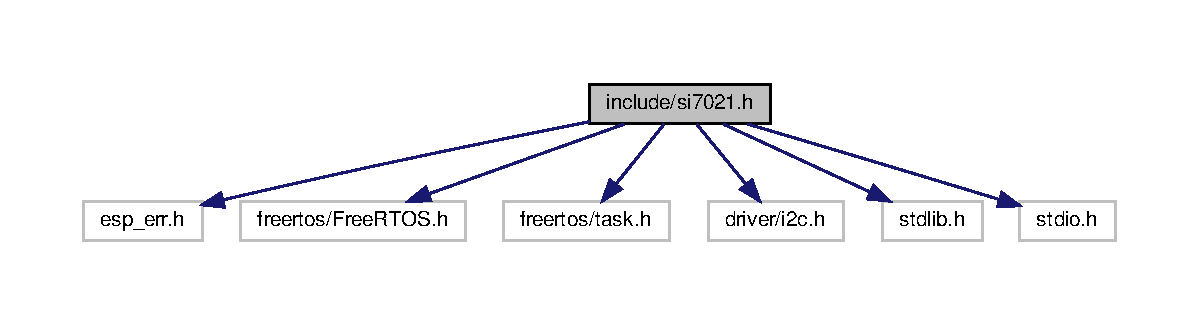
\includegraphics[width=350pt]{si7021_8h__incl}
\end{center}
\end{figure}
This graph shows which files directly or indirectly include this file\+:\nopagebreak
\begin{figure}[H]
\begin{center}
\leavevmode
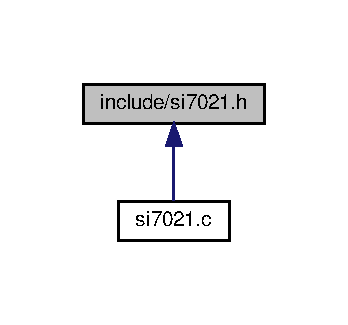
\includegraphics[width=167pt]{si7021_8h__dep__incl}
\end{center}
\end{figure}
\subsection*{Data Structures}
\begin{DoxyCompactItemize}
\item 
struct \hyperlink{structsi7021__config__t}{si7021\+\_\+config\+\_\+t}
\begin{DoxyCompactList}\small\item\em S\+I7021 initialization parameter. \end{DoxyCompactList}\end{DoxyCompactItemize}
\subsection*{Macros}
\begin{DoxyCompactItemize}
\item 
\#define \hyperlink{si7021_8h_ae2f3ab58a249649a0460ffe3826f8d60}{S\+I7021\+\_\+\+A\+D\+DR}~0x40
\item 
\#define \hyperlink{group__SI7021__I2C__CMD_ga999d78aa56f7bd9ce04bb52e691d6753}{S\+I7021\+\_\+\+M\+E\+A\+S\+R\+H\+\_\+\+H\+O\+L\+D\+\_\+\+C\+MD}~0x\+E5
\item 
\#define \hyperlink{group__SI7021__I2C__CMD_ga7982df3514be8aa0cfef6e87e0aa48b0}{S\+I7021\+\_\+\+M\+E\+A\+S\+R\+H\+\_\+\+N\+O\+H\+O\+L\+D\+\_\+\+C\+MD}~0x\+F5
\item 
\#define \hyperlink{group__SI7021__I2C__CMD_ga2afcdc38468c893701a91bbf41c3e3d5}{S\+I7021\+\_\+\+M\+E\+A\+S\+T\+E\+M\+P\+\_\+\+H\+O\+L\+D\+\_\+\+C\+MD}~0x\+E3
\item 
\#define \hyperlink{group__SI7021__I2C__CMD_gad008920c3e715fc4c63032daca3bc5b0}{S\+I7021\+\_\+\+M\+E\+A\+S\+T\+E\+M\+P\+\_\+\+N\+O\+H\+O\+L\+D\+\_\+\+C\+MD}~0x\+F3
\item 
\#define \hyperlink{group__SI7021__I2C__CMD_gaf69388821d62e94cccd567f8861743a3}{S\+I7021\+\_\+\+R\+E\+A\+D\+P\+R\+E\+V\+T\+E\+M\+P\+\_\+\+C\+MD}~0x\+E0
\item 
\#define \hyperlink{group__SI7021__I2C__CMD_gaf46ed75ac39abc8aa85a2f08f6eaf2fb}{S\+I7021\+\_\+\+R\+E\+S\+E\+T\+\_\+\+C\+MD}~0x\+FE
\item 
\#define \hyperlink{group__SI7021__I2C__CMD_gaec66f83a736566c680c195cad9f7cb7c}{S\+I7021\+\_\+\+W\+R\+I\+T\+E\+R\+H\+T\+\_\+\+R\+E\+G\+\_\+\+C\+MD}~0x\+E6
\item 
\#define \hyperlink{group__SI7021__I2C__CMD_ga39482cdbef1a96514a58d25c30cab869}{S\+I7021\+\_\+\+R\+E\+A\+D\+R\+H\+T\+\_\+\+R\+E\+G\+\_\+\+C\+MD}~0x\+E7
\item 
\#define \hyperlink{group__SI7021__I2C__CMD_gaf62a1fb7fe727aa31f52de3ce616e3a4}{S\+I7021\+\_\+\+W\+R\+I\+T\+E\+H\+E\+A\+T\+E\+R\+\_\+\+R\+E\+G\+\_\+\+C\+MD}~0x51
\item 
\#define \hyperlink{group__SI7021__I2C__CMD_ga3b1583b7a4599056347a0f8fea5349fa}{S\+I7021\+\_\+\+R\+E\+A\+D\+H\+E\+A\+T\+E\+R\+\_\+\+R\+E\+G\+\_\+\+C\+MD}~0x11
\item 
\#define \hyperlink{group__SI7021__I2C__CMD_ga4b71181e51a490ca8626758a80a0d14c}{S\+I7021\+\_\+\+I\+D1\+\_\+\+C\+MD}~0x\+F\+A0F
\item 
\#define \hyperlink{group__SI7021__I2C__CMD_ga65ab7ac27fe593eb11f4b0c4c9a16319}{S\+I7021\+\_\+\+I\+D2\+\_\+\+C\+MD}~0x\+F\+C\+C9
\item 
\#define \hyperlink{group__SI7021__I2C__CMD_ga2e429d79e5cca3c05d883b5509a88963}{S\+I7021\+\_\+\+F\+I\+R\+M\+V\+E\+R\+S\+\_\+\+C\+MD}~0x84\+B8
\item 
\#define \hyperlink{group__SI7021__I2C__CMD_ga6d880c26eb3b8bff87e47ee43dd5e8a4}{S\+I7021\+\_\+\+S\+O\+F\+T\+\_\+\+R\+E\+S\+E\+T\+\_\+\+C\+MD}~0x\+FE
\item 
\#define \hyperlink{group__SI7021__RT__VALUE_ga04cef12730209bc72277b64111308b42}{S\+I7021\+\_\+\+E\+R\+R\+\_\+\+OK}~0x00
\item 
\#define \hyperlink{group__SI7021__RT__VALUE_ga0abfa8d0b3297244d470fcdbce8e39da}{S\+I7021\+\_\+\+E\+R\+R\+\_\+\+C\+O\+N\+F\+IG}~0x01
\item 
\#define \hyperlink{group__SI7021__RT__VALUE_ga1a536c4aff63acd66547e006b587841b}{S\+I7021\+\_\+\+E\+R\+R\+\_\+\+I\+N\+S\+T\+A\+LL}~0x02
\item 
\#define \hyperlink{group__SI7021__RT__VALUE_ga277249c1e2c9ac97e4bec42c79ad4e49}{S\+I7021\+\_\+\+E\+R\+R\+\_\+\+N\+O\+T\+F\+O\+U\+ND}~0x03
\item 
\#define \hyperlink{group__SI7021__RT__VALUE_gad1c1ac433562f82e632c21f92c0fd4a3}{S\+I7021\+\_\+\+E\+R\+R\+\_\+\+I\+N\+V\+A\+L\+I\+D\+\_\+\+A\+RG}~0x04
\item 
\#define \hyperlink{group__SI7021__RT__VALUE_ga7cc0cccf705f1f1807d09abc3d1bea14}{S\+I7021\+\_\+\+E\+R\+R\+\_\+\+F\+A\+IL}~0x05
\item 
\#define \hyperlink{group__SI7021__RT__VALUE_gadf36521836ea146264b0db90fd02fb45}{S\+I7021\+\_\+\+E\+R\+R\+\_\+\+I\+N\+V\+A\+L\+I\+D\+\_\+\+S\+T\+A\+TE}~0x06
\item 
\#define \hyperlink{group__SI7021__RT__VALUE_gaf3c553ace8f63aa562e2263c47a1b5ed}{S\+I7021\+\_\+\+E\+R\+R\+\_\+\+T\+I\+M\+E\+O\+UT}~0x07
\item 
\#define \hyperlink{si7021_8h_af209481235e9da082e1447dc34478651}{S\+I7021\+\_\+\+H\+E\+A\+T\+E\+R\+\_\+\+ON}~0x01
\item 
\#define \hyperlink{si7021_8h_a7b49e55ef2f682cfe12cd29a09283e68}{S\+I7021\+\_\+\+H\+E\+A\+T\+E\+R\+\_\+\+O\+FF}~0x00
\end{DoxyCompactItemize}
\subsection*{Typedefs}
\begin{DoxyCompactItemize}
\item 
typedef enum \hyperlink{si7021_8h_ad2e0aa498b8faee91d8da4930f61625e}{S\+I7021\+\_\+\+R\+E\+S\+O\+L\+U\+T\+I\+ON} \hyperlink{si7021_8h_afd2b81672571b0b768341fc251a9965b}{S\+I7021\+\_\+\+R\+E\+S\+O\+L\+U\+T\+I\+ON}
\begin{DoxyCompactList}\small\item\em Enum contain all valid Resolution configuration of sensor. \end{DoxyCompactList}\item 
typedef enum \hyperlink{si7021_8h_ae8747642c3a83dd9ae9ae0333b84f9f3}{S\+I7021\+\_\+\+V\+D\+D\+\_\+\+S\+T\+A\+T\+US} \hyperlink{si7021_8h_a2ebdc2e1ec4e81de336c5441a6b11a0e}{S\+I7021\+\_\+\+V\+D\+D\+\_\+\+S\+T\+A\+T\+US}
\begin{DoxyCompactList}\small\item\em V\+DD status of sensor return type. \end{DoxyCompactList}\item 
typedef struct \hyperlink{structsi7021__config__t}{si7021\+\_\+config\+\_\+t} \hyperlink{si7021_8h_a3065c7b8861b54caafcedcdc032f0e02}{si7021\+\_\+config\+\_\+t}
\begin{DoxyCompactList}\small\item\em S\+I7021 initialization parameter. \end{DoxyCompactList}\item 
typedef uint8\+\_\+t \hyperlink{si7021_8h_aeec681879f00b18fe17bddc989b9582d}{si7021\+\_\+err\+\_\+t}
\begin{DoxyCompactList}\small\item\em Error type for return value. \end{DoxyCompactList}\end{DoxyCompactItemize}
\subsection*{Enumerations}
\begin{DoxyCompactItemize}
\item 
enum \hyperlink{si7021_8h_ad2e0aa498b8faee91d8da4930f61625e}{S\+I7021\+\_\+\+R\+E\+S\+O\+L\+U\+T\+I\+ON} \{ \hyperlink{si7021_8h_ad2e0aa498b8faee91d8da4930f61625eaf7e31fbc799b25fdc172fb9d6c01ae84}{S\+I7021\+\_\+12\+\_\+14\+\_\+\+R\+ES} = 0x00, 
\hyperlink{si7021_8h_ad2e0aa498b8faee91d8da4930f61625ea3f096d60050714a92d1889dbb9d4ba8a}{S\+I7021\+\_\+8\+\_\+12\+\_\+\+R\+ES} = 0x01, 
\hyperlink{si7021_8h_ad2e0aa498b8faee91d8da4930f61625ea2cfafb4c2314cb0c4a4ee0f840f5f3a1}{S\+I7021\+\_\+10\+\_\+13\+\_\+\+R\+ES} = 0x80, 
\hyperlink{si7021_8h_ad2e0aa498b8faee91d8da4930f61625ea7db14da7bc2b59132110df783f3b31b0}{S\+I7021\+\_\+11\+\_\+11\+\_\+\+R\+ES} = 0x81
 \}\begin{DoxyCompactList}\small\item\em Enum contain all valid Resolution configuration of sensor. \end{DoxyCompactList}
\item 
enum \hyperlink{si7021_8h_ae8747642c3a83dd9ae9ae0333b84f9f3}{S\+I7021\+\_\+\+V\+D\+D\+\_\+\+S\+T\+A\+T\+US} \{ \hyperlink{si7021_8h_ae8747642c3a83dd9ae9ae0333b84f9f3acdfe83b75cad583ca9ee2997322174ea}{S\+I7021\+\_\+\+V\+D\+D\+\_\+\+OK} = 0x01, 
\hyperlink{si7021_8h_ae8747642c3a83dd9ae9ae0333b84f9f3a1ad64fa668e0c9b079a23971c4bb1505}{S\+I7021\+\_\+\+V\+D\+D\+\_\+\+L\+OW} = 0x00
 \}\begin{DoxyCompactList}\small\item\em V\+DD status of sensor return type. \end{DoxyCompactList}
\end{DoxyCompactItemize}
\subsection*{Functions}
\begin{DoxyCompactItemize}
\item 
\hyperlink{si7021_8h_aeec681879f00b18fe17bddc989b9582d}{si7021\+\_\+err\+\_\+t} \hyperlink{si7021_8h_a82f9c8e22626638e47729098f8493c1f}{si7021\+\_\+init} (\hyperlink{structsi7021__config__t}{si7021\+\_\+config\+\_\+t} $\ast$config)
\begin{DoxyCompactList}\small\item\em Initialize S\+I7021 sensor. \end{DoxyCompactList}\item 
\hyperlink{si7021_8h_aeec681879f00b18fe17bddc989b9582d}{si7021\+\_\+err\+\_\+t} \hyperlink{si7021_8h_a339f08aa1ed1d74c2c12fd904ea4e28c}{\+\_\+\+\_\+si7021\+\_\+param\+\_\+config} (\hyperlink{structsi7021__config__t}{si7021\+\_\+config\+\_\+t} $\ast$config)
\begin{DoxyCompactList}\small\item\em Configure I2C Parameter for S\+I7021. \end{DoxyCompactList}\item 
\hyperlink{si7021_8h_aeec681879f00b18fe17bddc989b9582d}{si7021\+\_\+err\+\_\+t} \hyperlink{si7021_8h_a814069add0f4e59b5f254732d37637bf}{\+\_\+\+\_\+si7021\+\_\+driver\+\_\+config} (\hyperlink{structsi7021__config__t}{si7021\+\_\+config\+\_\+t} $\ast$config)
\begin{DoxyCompactList}\small\item\em Configure I2C Driver for S\+I7021. \end{DoxyCompactList}\item 
uint16\+\_\+t \hyperlink{si7021_8h_a06d36b1f00051ed948cf054b4700d1ec}{\+\_\+\+\_\+si7021\+\_\+read} (uint8\+\_\+t cmd)
\begin{DoxyCompactList}\small\item\em Get data from sensors by issuing read command and read data return by sensor. \end{DoxyCompactList}\item 
bool \hyperlink{si7021_8h_afee080ad732330932eed4d9d1d93b45f}{\+\_\+\+\_\+is\+\_\+crc\+\_\+valid} (uint16\+\_\+t value, uint8\+\_\+t crc)
\begin{DoxyCompactList}\small\item\em Check data integrity with crc. \end{DoxyCompactList}\item 
\hyperlink{si7021_8h_aeec681879f00b18fe17bddc989b9582d}{si7021\+\_\+err\+\_\+t} \hyperlink{si7021_8h_a17554408b2bda4f9219d479946e30fbb}{si7021\+\_\+check\+\_\+availability} ()
\begin{DoxyCompactList}\small\item\em Check the availability of sensor. \end{DoxyCompactList}\item 
float \hyperlink{si7021_8h_aac2b7c97826cdeb499ac224a8120fee2}{si7021\+\_\+read\+\_\+temperature} ()
\begin{DoxyCompactList}\small\item\em Read temperature value from sensor. \end{DoxyCompactList}\item 
float \hyperlink{si7021_8h_afebf7dfa4b71f1d0848955edf97a8156}{si7021\+\_\+read\+\_\+humidity} ()
\begin{DoxyCompactList}\small\item\em Read \href{https://en.wikipedia.org/wiki/Relative_humidity}{\tt Relative Humidity} value from sensor. \end{DoxyCompactList}\item 
uint8\+\_\+t \hyperlink{si7021_8h_a91041d121bd0dff34dc9383479286e2d}{\+\_\+\+\_\+si7021\+\_\+read\+\_\+user\+\_\+register} ()
\begin{DoxyCompactList}\small\item\em Read R\+H/T user register 1 from sensor. \end{DoxyCompactList}\item 
\hyperlink{si7021_8h_aeec681879f00b18fe17bddc989b9582d}{si7021\+\_\+err\+\_\+t} \hyperlink{si7021_8h_ab01f45ffce7fdfa1f150f4b3f15c4e33}{\+\_\+\+\_\+si7021\+\_\+write\+\_\+user\+\_\+register} (uint8\+\_\+t value)
\begin{DoxyCompactList}\small\item\em Write value to R\+H/T user register 1. \end{DoxyCompactList}\item 
\hyperlink{si7021_8h_ad2e0aa498b8faee91d8da4930f61625e}{S\+I7021\+\_\+\+R\+E\+S\+O\+L\+U\+T\+I\+ON} \hyperlink{si7021_8h_a7347c3be7bfb07b492e4cbed1cdbcfb9}{si7021\+\_\+get\+\_\+resolution} ()
\begin{DoxyCompactList}\small\item\em Get current resolution of sensor. \end{DoxyCompactList}\item 
\hyperlink{si7021_8h_aeec681879f00b18fe17bddc989b9582d}{si7021\+\_\+err\+\_\+t} \hyperlink{si7021_8h_a7800e376fe6c29d695e3dd36ad28a1e9}{si7021\+\_\+soft\+\_\+reset} ()
\begin{DoxyCompactList}\small\item\em Reset the sensor. \end{DoxyCompactList}\item 
\hyperlink{si7021_8h_aeec681879f00b18fe17bddc989b9582d}{si7021\+\_\+err\+\_\+t} \hyperlink{si7021_8h_afd590ce231e3b83309411c505af7e169}{si7021\+\_\+set\+\_\+resolution} (\hyperlink{si7021_8h_ad2e0aa498b8faee91d8da4930f61625e}{S\+I7021\+\_\+\+R\+E\+S\+O\+L\+U\+T\+I\+ON} resolution)
\begin{DoxyCompactList}\small\item\em Set the sensors resolution. \end{DoxyCompactList}\item 
\hyperlink{si7021_8h_aeec681879f00b18fe17bddc989b9582d}{si7021\+\_\+err\+\_\+t} \hyperlink{si7021_8h_ab4db1385ee975ed53c1b4cb8b2f82da7}{si7021\+\_\+set\+\_\+heater\+\_\+register} (uint8\+\_\+t value)
\begin{DoxyCompactList}\small\item\em Set heater register. \end{DoxyCompactList}\item 
\hyperlink{si7021_8h_aeec681879f00b18fe17bddc989b9582d}{si7021\+\_\+err\+\_\+t} \hyperlink{si7021_8h_a65fe3b1e33bdbebf8df2c8d51bbbf675}{si7021\+\_\+set\+\_\+heater\+\_\+status} (uint8\+\_\+t value)
\begin{DoxyCompactList}\small\item\em Set heater status. \end{DoxyCompactList}\item 
uint8\+\_\+t \hyperlink{si7021_8h_ad85d7885ebbb87e1ac1f12b78a6c0af7}{si7021\+\_\+get\+\_\+heater\+\_\+register} ()
\begin{DoxyCompactList}\small\item\em Read heater register. \end{DoxyCompactList}\item 
uint8\+\_\+t \hyperlink{si7021_8h_a1e1e3955782fa3079544f048d42ad88e}{si7021\+\_\+read\+\_\+firmware\+\_\+rev} ()
\begin{DoxyCompactList}\small\item\em Read sensor firmware revision. \end{DoxyCompactList}\item 
\hyperlink{si7021_8h_ae8747642c3a83dd9ae9ae0333b84f9f3}{S\+I7021\+\_\+\+V\+D\+D\+\_\+\+S\+T\+A\+T\+US} \hyperlink{si7021_8h_a5b42332bda6837327d02700bbaca7060}{si7021\+\_\+read\+\_\+vdd\+\_\+status} ()
\begin{DoxyCompactList}\small\item\em Check sensors V\+DD. \end{DoxyCompactList}\item 
uint8\+\_\+t \hyperlink{si7021_8h_a6ec069cec3b96b638c8f0426aca309b2}{si7021\+\_\+get\+\_\+heater\+\_\+status} ()
\begin{DoxyCompactList}\small\item\em Check sensors heater status. \end{DoxyCompactList}\item 
uint64\+\_\+t \hyperlink{si7021_8h_ab0d521e94113c17457f8898e37410009}{get\+\_\+electronic\+\_\+id} ()
\begin{DoxyCompactList}\small\item\em Get sensor electronic id. \end{DoxyCompactList}\end{DoxyCompactItemize}
\subsection*{Variables}
\begin{DoxyCompactItemize}
\item 
\hyperlink{structsi7021__config__t}{si7021\+\_\+config\+\_\+t} \hyperlink{si7021_8h_a7961a32ca6f5fed329358f12119b97b6}{\+\_\+\+\_\+si7021\+\_\+config}
\begin{DoxyCompactList}\small\item\em Internal variable for storing sensor information. \end{DoxyCompactList}\end{DoxyCompactItemize}


\subsection{Detailed Description}
S\+I7021 Library for E\+S\+P-\/\+I\+DF framework header file. 

\begin{DoxyAuthor}{Author}
Le Nguyen Hoang Nhan 
\end{DoxyAuthor}
\begin{DoxyDate}{Date}
19 May 2019
\end{DoxyDate}
\begin{DoxySeeAlso}{See also}
\href{https://www.silabs.com/documents/public/data-sheets/Si7021-A20.pdf}{\tt https\+://www.\+silabs.\+com/documents/public/data-\/sheets/\+Si7021-\/\+A20.\+pdf} 
\end{DoxySeeAlso}
\begin{DoxyCopyright}{Copyright}
Copyright (C) 2019 Le Nguyen Hoang Nhan. All rights reserved. 
\end{DoxyCopyright}


\subsection{Macro Definition Documentation}
\mbox{\Hypertarget{si7021_8h_ae2f3ab58a249649a0460ffe3826f8d60}\label{si7021_8h_ae2f3ab58a249649a0460ffe3826f8d60}} 
\index{si7021.\+h@{si7021.\+h}!S\+I7021\+\_\+\+A\+D\+DR@{S\+I7021\+\_\+\+A\+D\+DR}}
\index{S\+I7021\+\_\+\+A\+D\+DR@{S\+I7021\+\_\+\+A\+D\+DR}!si7021.\+h@{si7021.\+h}}
\subsubsection{\texorpdfstring{S\+I7021\+\_\+\+A\+D\+DR}{SI7021\_ADDR}}
{\footnotesize\ttfamily \#define S\+I7021\+\_\+\+A\+D\+DR~0x40}

S\+I7021 default address 

Definition at line 41 of file si7021.\+h.



Referenced by \+\_\+\+\_\+si7021\+\_\+read(), \+\_\+\+\_\+si7021\+\_\+read\+\_\+user\+\_\+register(), \+\_\+\+\_\+si7021\+\_\+write\+\_\+user\+\_\+register(), get\+\_\+electronic\+\_\+id(), si7021\+\_\+check\+\_\+availability(), si7021\+\_\+get\+\_\+heater\+\_\+register(), si7021\+\_\+read\+\_\+firmware\+\_\+rev(), si7021\+\_\+set\+\_\+heater\+\_\+register(), and si7021\+\_\+soft\+\_\+reset().

\mbox{\Hypertarget{si7021_8h_a7b49e55ef2f682cfe12cd29a09283e68}\label{si7021_8h_a7b49e55ef2f682cfe12cd29a09283e68}} 
\index{si7021.\+h@{si7021.\+h}!S\+I7021\+\_\+\+H\+E\+A\+T\+E\+R\+\_\+\+O\+FF@{S\+I7021\+\_\+\+H\+E\+A\+T\+E\+R\+\_\+\+O\+FF}}
\index{S\+I7021\+\_\+\+H\+E\+A\+T\+E\+R\+\_\+\+O\+FF@{S\+I7021\+\_\+\+H\+E\+A\+T\+E\+R\+\_\+\+O\+FF}!si7021.\+h@{si7021.\+h}}
\subsubsection{\texorpdfstring{S\+I7021\+\_\+\+H\+E\+A\+T\+E\+R\+\_\+\+O\+FF}{SI7021\_HEATER\_OFF}}
{\footnotesize\ttfamily \#define S\+I7021\+\_\+\+H\+E\+A\+T\+E\+R\+\_\+\+O\+FF~0x00}

Heater is O\+FF 

Definition at line 103 of file si7021.\+h.



Referenced by si7021\+\_\+get\+\_\+heater\+\_\+status(), and si7021\+\_\+set\+\_\+heater\+\_\+status().

\mbox{\Hypertarget{si7021_8h_af209481235e9da082e1447dc34478651}\label{si7021_8h_af209481235e9da082e1447dc34478651}} 
\index{si7021.\+h@{si7021.\+h}!S\+I7021\+\_\+\+H\+E\+A\+T\+E\+R\+\_\+\+ON@{S\+I7021\+\_\+\+H\+E\+A\+T\+E\+R\+\_\+\+ON}}
\index{S\+I7021\+\_\+\+H\+E\+A\+T\+E\+R\+\_\+\+ON@{S\+I7021\+\_\+\+H\+E\+A\+T\+E\+R\+\_\+\+ON}!si7021.\+h@{si7021.\+h}}
\subsubsection{\texorpdfstring{S\+I7021\+\_\+\+H\+E\+A\+T\+E\+R\+\_\+\+ON}{SI7021\_HEATER\_ON}}
{\footnotesize\ttfamily \#define S\+I7021\+\_\+\+H\+E\+A\+T\+E\+R\+\_\+\+ON~0x01}

Heater is ON 

Definition at line 102 of file si7021.\+h.



Referenced by si7021\+\_\+get\+\_\+heater\+\_\+status(), and si7021\+\_\+set\+\_\+heater\+\_\+status().



\subsection{Typedef Documentation}
\mbox{\Hypertarget{si7021_8h_a3065c7b8861b54caafcedcdc032f0e02}\label{si7021_8h_a3065c7b8861b54caafcedcdc032f0e02}} 
\index{si7021.\+h@{si7021.\+h}!si7021\+\_\+config\+\_\+t@{si7021\+\_\+config\+\_\+t}}
\index{si7021\+\_\+config\+\_\+t@{si7021\+\_\+config\+\_\+t}!si7021.\+h@{si7021.\+h}}
\subsubsection{\texorpdfstring{si7021\+\_\+config\+\_\+t}{si7021\_config\_t}}
{\footnotesize\ttfamily typedef struct \hyperlink{structsi7021__config__t}{si7021\+\_\+config\+\_\+t}  \hyperlink{structsi7021__config__t}{si7021\+\_\+config\+\_\+t}}



S\+I7021 initialization parameter. 

\begin{DoxySeeAlso}{See also}
\hyperlink{si7021_8c_a7961a32ca6f5fed329358f12119b97b6}{\+\_\+\+\_\+si7021\+\_\+config} 

i2c.\+h\+::i2c\+\_\+config\+\_\+t 
\end{DoxySeeAlso}
\mbox{\Hypertarget{si7021_8h_aeec681879f00b18fe17bddc989b9582d}\label{si7021_8h_aeec681879f00b18fe17bddc989b9582d}} 
\index{si7021.\+h@{si7021.\+h}!si7021\+\_\+err\+\_\+t@{si7021\+\_\+err\+\_\+t}}
\index{si7021\+\_\+err\+\_\+t@{si7021\+\_\+err\+\_\+t}!si7021.\+h@{si7021.\+h}}
\subsubsection{\texorpdfstring{si7021\+\_\+err\+\_\+t}{si7021\_err\_t}}
{\footnotesize\ttfamily typedef uint8\+\_\+t \hyperlink{si7021_8h_aeec681879f00b18fe17bddc989b9582d}{si7021\+\_\+err\+\_\+t}}



Error type for return value. 



Definition at line 121 of file si7021.\+h.

\mbox{\Hypertarget{si7021_8h_afd2b81672571b0b768341fc251a9965b}\label{si7021_8h_afd2b81672571b0b768341fc251a9965b}} 
\index{si7021.\+h@{si7021.\+h}!S\+I7021\+\_\+\+R\+E\+S\+O\+L\+U\+T\+I\+ON@{S\+I7021\+\_\+\+R\+E\+S\+O\+L\+U\+T\+I\+ON}}
\index{S\+I7021\+\_\+\+R\+E\+S\+O\+L\+U\+T\+I\+ON@{S\+I7021\+\_\+\+R\+E\+S\+O\+L\+U\+T\+I\+ON}!si7021.\+h@{si7021.\+h}}
\subsubsection{\texorpdfstring{S\+I7021\+\_\+\+R\+E\+S\+O\+L\+U\+T\+I\+ON}{SI7021\_RESOLUTION}}
{\footnotesize\ttfamily typedef enum \hyperlink{si7021_8h_ad2e0aa498b8faee91d8da4930f61625e}{S\+I7021\+\_\+\+R\+E\+S\+O\+L\+U\+T\+I\+ON} \hyperlink{si7021_8h_ad2e0aa498b8faee91d8da4930f61625e}{S\+I7021\+\_\+\+R\+E\+S\+O\+L\+U\+T\+I\+ON}}



Enum contain all valid Resolution configuration of sensor. 

\begin{DoxyNote}{Note}
Only bit 0 and bit 7 matter, other bits will be ignored 
\end{DoxyNote}
\mbox{\Hypertarget{si7021_8h_a2ebdc2e1ec4e81de336c5441a6b11a0e}\label{si7021_8h_a2ebdc2e1ec4e81de336c5441a6b11a0e}} 
\index{si7021.\+h@{si7021.\+h}!S\+I7021\+\_\+\+V\+D\+D\+\_\+\+S\+T\+A\+T\+US@{S\+I7021\+\_\+\+V\+D\+D\+\_\+\+S\+T\+A\+T\+US}}
\index{S\+I7021\+\_\+\+V\+D\+D\+\_\+\+S\+T\+A\+T\+US@{S\+I7021\+\_\+\+V\+D\+D\+\_\+\+S\+T\+A\+T\+US}!si7021.\+h@{si7021.\+h}}
\subsubsection{\texorpdfstring{S\+I7021\+\_\+\+V\+D\+D\+\_\+\+S\+T\+A\+T\+US}{SI7021\_VDD\_STATUS}}
{\footnotesize\ttfamily typedef enum \hyperlink{si7021_8h_ae8747642c3a83dd9ae9ae0333b84f9f3}{S\+I7021\+\_\+\+V\+D\+D\+\_\+\+S\+T\+A\+T\+US}  \hyperlink{si7021_8h_ae8747642c3a83dd9ae9ae0333b84f9f3}{S\+I7021\+\_\+\+V\+D\+D\+\_\+\+S\+T\+A\+T\+US}}



V\+DD status of sensor return type. 

\begin{DoxyNote}{Note}
Consider changing power supply if V\+DD is L\+OW, the sensor may not work correctly 
\end{DoxyNote}


\subsection{Enumeration Type Documentation}
\mbox{\Hypertarget{si7021_8h_ad2e0aa498b8faee91d8da4930f61625e}\label{si7021_8h_ad2e0aa498b8faee91d8da4930f61625e}} 
\index{si7021.\+h@{si7021.\+h}!S\+I7021\+\_\+\+R\+E\+S\+O\+L\+U\+T\+I\+ON@{S\+I7021\+\_\+\+R\+E\+S\+O\+L\+U\+T\+I\+ON}}
\index{S\+I7021\+\_\+\+R\+E\+S\+O\+L\+U\+T\+I\+ON@{S\+I7021\+\_\+\+R\+E\+S\+O\+L\+U\+T\+I\+ON}!si7021.\+h@{si7021.\+h}}
\subsubsection{\texorpdfstring{S\+I7021\+\_\+\+R\+E\+S\+O\+L\+U\+T\+I\+ON}{SI7021\_RESOLUTION}}
{\footnotesize\ttfamily enum \hyperlink{si7021_8h_ad2e0aa498b8faee91d8da4930f61625e}{S\+I7021\+\_\+\+R\+E\+S\+O\+L\+U\+T\+I\+ON}}



Enum contain all valid Resolution configuration of sensor. 

\begin{DoxyNote}{Note}
Only bit 0 and bit 7 matter, other bits will be ignored 
\end{DoxyNote}
\begin{DoxyEnumFields}{Enumerator}
\raisebox{\heightof{T}}[0pt][0pt]{\index{S\+I7021\+\_\+12\+\_\+14\+\_\+\+R\+ES@{S\+I7021\+\_\+12\+\_\+14\+\_\+\+R\+ES}!si7021.\+h@{si7021.\+h}}\index{si7021.\+h@{si7021.\+h}!S\+I7021\+\_\+12\+\_\+14\+\_\+\+R\+ES@{S\+I7021\+\_\+12\+\_\+14\+\_\+\+R\+ES}}}\mbox{\Hypertarget{si7021_8h_ad2e0aa498b8faee91d8da4930f61625eaf7e31fbc799b25fdc172fb9d6c01ae84}\label{si7021_8h_ad2e0aa498b8faee91d8da4930f61625eaf7e31fbc799b25fdc172fb9d6c01ae84}} 
S\+I7021\+\_\+12\+\_\+14\+\_\+\+R\+ES&12bit RH resolution, 14bit temperature resolution \\
\hline

\raisebox{\heightof{T}}[0pt][0pt]{\index{S\+I7021\+\_\+8\+\_\+12\+\_\+\+R\+ES@{S\+I7021\+\_\+8\+\_\+12\+\_\+\+R\+ES}!si7021.\+h@{si7021.\+h}}\index{si7021.\+h@{si7021.\+h}!S\+I7021\+\_\+8\+\_\+12\+\_\+\+R\+ES@{S\+I7021\+\_\+8\+\_\+12\+\_\+\+R\+ES}}}\mbox{\Hypertarget{si7021_8h_ad2e0aa498b8faee91d8da4930f61625ea3f096d60050714a92d1889dbb9d4ba8a}\label{si7021_8h_ad2e0aa498b8faee91d8da4930f61625ea3f096d60050714a92d1889dbb9d4ba8a}} 
S\+I7021\+\_\+8\+\_\+12\+\_\+\+R\+ES&8bit RH resolution, 12bit temperature resolution \\
\hline

\raisebox{\heightof{T}}[0pt][0pt]{\index{S\+I7021\+\_\+10\+\_\+13\+\_\+\+R\+ES@{S\+I7021\+\_\+10\+\_\+13\+\_\+\+R\+ES}!si7021.\+h@{si7021.\+h}}\index{si7021.\+h@{si7021.\+h}!S\+I7021\+\_\+10\+\_\+13\+\_\+\+R\+ES@{S\+I7021\+\_\+10\+\_\+13\+\_\+\+R\+ES}}}\mbox{\Hypertarget{si7021_8h_ad2e0aa498b8faee91d8da4930f61625ea2cfafb4c2314cb0c4a4ee0f840f5f3a1}\label{si7021_8h_ad2e0aa498b8faee91d8da4930f61625ea2cfafb4c2314cb0c4a4ee0f840f5f3a1}} 
S\+I7021\+\_\+10\+\_\+13\+\_\+\+R\+ES&10bit RH resolution, 13bit temperature resolution \\
\hline

\raisebox{\heightof{T}}[0pt][0pt]{\index{S\+I7021\+\_\+11\+\_\+11\+\_\+\+R\+ES@{S\+I7021\+\_\+11\+\_\+11\+\_\+\+R\+ES}!si7021.\+h@{si7021.\+h}}\index{si7021.\+h@{si7021.\+h}!S\+I7021\+\_\+11\+\_\+11\+\_\+\+R\+ES@{S\+I7021\+\_\+11\+\_\+11\+\_\+\+R\+ES}}}\mbox{\Hypertarget{si7021_8h_ad2e0aa498b8faee91d8da4930f61625ea7db14da7bc2b59132110df783f3b31b0}\label{si7021_8h_ad2e0aa498b8faee91d8da4930f61625ea7db14da7bc2b59132110df783f3b31b0}} 
S\+I7021\+\_\+11\+\_\+11\+\_\+\+R\+ES&11bit RH resolution, 11bit temperature resolution \\
\hline

\end{DoxyEnumFields}


Definition at line 87 of file si7021.\+h.

\mbox{\Hypertarget{si7021_8h_ae8747642c3a83dd9ae9ae0333b84f9f3}\label{si7021_8h_ae8747642c3a83dd9ae9ae0333b84f9f3}} 
\index{si7021.\+h@{si7021.\+h}!S\+I7021\+\_\+\+V\+D\+D\+\_\+\+S\+T\+A\+T\+US@{S\+I7021\+\_\+\+V\+D\+D\+\_\+\+S\+T\+A\+T\+US}}
\index{S\+I7021\+\_\+\+V\+D\+D\+\_\+\+S\+T\+A\+T\+US@{S\+I7021\+\_\+\+V\+D\+D\+\_\+\+S\+T\+A\+T\+US}!si7021.\+h@{si7021.\+h}}
\subsubsection{\texorpdfstring{S\+I7021\+\_\+\+V\+D\+D\+\_\+\+S\+T\+A\+T\+US}{SI7021\_VDD\_STATUS}}
{\footnotesize\ttfamily enum \hyperlink{si7021_8h_ae8747642c3a83dd9ae9ae0333b84f9f3}{S\+I7021\+\_\+\+V\+D\+D\+\_\+\+S\+T\+A\+T\+US}}



V\+DD status of sensor return type. 

\begin{DoxyNote}{Note}
Consider changing power supply if V\+DD is L\+OW, the sensor may not work correctly 
\end{DoxyNote}
\begin{DoxyEnumFields}{Enumerator}
\raisebox{\heightof{T}}[0pt][0pt]{\index{S\+I7021\+\_\+\+V\+D\+D\+\_\+\+OK@{S\+I7021\+\_\+\+V\+D\+D\+\_\+\+OK}!si7021.\+h@{si7021.\+h}}\index{si7021.\+h@{si7021.\+h}!S\+I7021\+\_\+\+V\+D\+D\+\_\+\+OK@{S\+I7021\+\_\+\+V\+D\+D\+\_\+\+OK}}}\mbox{\Hypertarget{si7021_8h_ae8747642c3a83dd9ae9ae0333b84f9f3acdfe83b75cad583ca9ee2997322174ea}\label{si7021_8h_ae8747642c3a83dd9ae9ae0333b84f9f3acdfe83b75cad583ca9ee2997322174ea}} 
S\+I7021\+\_\+\+V\+D\+D\+\_\+\+OK&V\+DD is OK ($>$1.\+9 V) \\
\hline

\raisebox{\heightof{T}}[0pt][0pt]{\index{S\+I7021\+\_\+\+V\+D\+D\+\_\+\+L\+OW@{S\+I7021\+\_\+\+V\+D\+D\+\_\+\+L\+OW}!si7021.\+h@{si7021.\+h}}\index{si7021.\+h@{si7021.\+h}!S\+I7021\+\_\+\+V\+D\+D\+\_\+\+L\+OW@{S\+I7021\+\_\+\+V\+D\+D\+\_\+\+L\+OW}}}\mbox{\Hypertarget{si7021_8h_ae8747642c3a83dd9ae9ae0333b84f9f3a1ad64fa668e0c9b079a23971c4bb1505}\label{si7021_8h_ae8747642c3a83dd9ae9ae0333b84f9f3a1ad64fa668e0c9b079a23971c4bb1505}} 
S\+I7021\+\_\+\+V\+D\+D\+\_\+\+L\+OW&V\+DD is L\+OW (1.\+9$\sim$1.8V) \\
\hline

\end{DoxyEnumFields}


Definition at line 97 of file si7021.\+h.



\subsection{Function Documentation}
\mbox{\Hypertarget{si7021_8h_afee080ad732330932eed4d9d1d93b45f}\label{si7021_8h_afee080ad732330932eed4d9d1d93b45f}} 
\index{si7021.\+h@{si7021.\+h}!\+\_\+\+\_\+is\+\_\+crc\+\_\+valid@{\+\_\+\+\_\+is\+\_\+crc\+\_\+valid}}
\index{\+\_\+\+\_\+is\+\_\+crc\+\_\+valid@{\+\_\+\+\_\+is\+\_\+crc\+\_\+valid}!si7021.\+h@{si7021.\+h}}
\subsubsection{\texorpdfstring{\+\_\+\+\_\+is\+\_\+crc\+\_\+valid()}{\_\_is\_crc\_valid()}}
{\footnotesize\ttfamily bool \+\_\+\+\_\+is\+\_\+crc\+\_\+valid (\begin{DoxyParamCaption}\item[{uint16\+\_\+t}]{value,  }\item[{uint8\+\_\+t}]{crc }\end{DoxyParamCaption})}



Check data integrity with crc. 


\begin{DoxyParams}{Parameters}
{\em value} & 16bit (uint16\+\_\+t) value that contain data return by sensors. \\
\hline
{\em crc} & 8bit (uint8\+\_\+t) value of crc data \\
\hline
\end{DoxyParams}
\begin{DoxyReturn}{Returns}

\begin{DoxyItemize}
\item boolean value, true if crc value is valid, otherwise false 
\end{DoxyItemize}
\end{DoxyReturn}


Definition at line 142 of file si7021.\+c.



Referenced by \+\_\+\+\_\+si7021\+\_\+read().

\mbox{\Hypertarget{si7021_8h_a814069add0f4e59b5f254732d37637bf}\label{si7021_8h_a814069add0f4e59b5f254732d37637bf}} 
\index{si7021.\+h@{si7021.\+h}!\+\_\+\+\_\+si7021\+\_\+driver\+\_\+config@{\+\_\+\+\_\+si7021\+\_\+driver\+\_\+config}}
\index{\+\_\+\+\_\+si7021\+\_\+driver\+\_\+config@{\+\_\+\+\_\+si7021\+\_\+driver\+\_\+config}!si7021.\+h@{si7021.\+h}}
\subsubsection{\texorpdfstring{\+\_\+\+\_\+si7021\+\_\+driver\+\_\+config()}{\_\_si7021\_driver\_config()}}
{\footnotesize\ttfamily \hyperlink{si7021_8h_aeec681879f00b18fe17bddc989b9582d}{si7021\+\_\+err\+\_\+t} \+\_\+\+\_\+si7021\+\_\+driver\+\_\+config (\begin{DoxyParamCaption}\item[{\hyperlink{structsi7021__config__t}{si7021\+\_\+config\+\_\+t} $\ast$}]{config }\end{DoxyParamCaption})}



Configure I2C Driver for S\+I7021. 

\begin{DoxyNote}{Note}
Internal use only 
\end{DoxyNote}

\begin{DoxyParams}{Parameters}
{\em config} & Forwarded parameter from \hyperlink{si7021_8h_a82f9c8e22626638e47729098f8493c1f}{si7021\+\_\+init}(\hyperlink{structsi7021__config__t}{si7021\+\_\+config\+\_\+t} $\ast$config) \\
\hline
\end{DoxyParams}
\begin{DoxyReturn}{Returns}

\begin{DoxyItemize}
\item \hyperlink{group__SI7021__RT__VALUE_ga04cef12730209bc72277b64111308b42}{S\+I7021\+\_\+\+E\+R\+R\+\_\+\+OK} Success
\item \hyperlink{group__SI7021__RT__VALUE_ga0abfa8d0b3297244d470fcdbce8e39da}{S\+I7021\+\_\+\+E\+R\+R\+\_\+\+C\+O\+N\+F\+IG} Failed to install I2C parameters 
\end{DoxyItemize}
\end{DoxyReturn}


Definition at line 61 of file si7021.\+c.



References S\+I7021\+\_\+\+E\+R\+R\+\_\+\+I\+N\+S\+T\+A\+LL, S\+I7021\+\_\+\+E\+R\+R\+\_\+\+OK, and si7021\+\_\+config\+\_\+t\+::si7021\+\_\+port.



Referenced by si7021\+\_\+init().

\mbox{\Hypertarget{si7021_8h_a339f08aa1ed1d74c2c12fd904ea4e28c}\label{si7021_8h_a339f08aa1ed1d74c2c12fd904ea4e28c}} 
\index{si7021.\+h@{si7021.\+h}!\+\_\+\+\_\+si7021\+\_\+param\+\_\+config@{\+\_\+\+\_\+si7021\+\_\+param\+\_\+config}}
\index{\+\_\+\+\_\+si7021\+\_\+param\+\_\+config@{\+\_\+\+\_\+si7021\+\_\+param\+\_\+config}!si7021.\+h@{si7021.\+h}}
\subsubsection{\texorpdfstring{\+\_\+\+\_\+si7021\+\_\+param\+\_\+config()}{\_\_si7021\_param\_config()}}
{\footnotesize\ttfamily \hyperlink{si7021_8h_aeec681879f00b18fe17bddc989b9582d}{si7021\+\_\+err\+\_\+t} \+\_\+\+\_\+si7021\+\_\+param\+\_\+config (\begin{DoxyParamCaption}\item[{\hyperlink{structsi7021__config__t}{si7021\+\_\+config\+\_\+t} $\ast$}]{config }\end{DoxyParamCaption})}



Configure I2C Parameter for S\+I7021. 

\begin{DoxyNote}{Note}
Internal use only 
\end{DoxyNote}

\begin{DoxyParams}{Parameters}
{\em config} & Forwarded parameter from \hyperlink{si7021_8h_a82f9c8e22626638e47729098f8493c1f}{si7021\+\_\+init}(\hyperlink{structsi7021__config__t}{si7021\+\_\+config\+\_\+t} $\ast$config) \\
\hline
\end{DoxyParams}
\begin{DoxyReturn}{Returns}

\begin{DoxyItemize}
\item \hyperlink{group__SI7021__RT__VALUE_ga04cef12730209bc72277b64111308b42}{S\+I7021\+\_\+\+E\+R\+R\+\_\+\+OK} Success.
\item \hyperlink{group__SI7021__RT__VALUE_ga0abfa8d0b3297244d470fcdbce8e39da}{S\+I7021\+\_\+\+E\+R\+R\+\_\+\+C\+O\+N\+F\+IG} Failed to configure I2C parameter 
\end{DoxyItemize}
\end{DoxyReturn}


Definition at line 50 of file si7021.\+c.



References si7021\+\_\+config\+\_\+t\+::sensors\+\_\+config, S\+I7021\+\_\+\+E\+R\+R\+\_\+\+C\+O\+N\+F\+IG, S\+I7021\+\_\+\+E\+R\+R\+\_\+\+OK, and si7021\+\_\+config\+\_\+t\+::si7021\+\_\+port.



Referenced by si7021\+\_\+init().

\mbox{\Hypertarget{si7021_8h_a06d36b1f00051ed948cf054b4700d1ec}\label{si7021_8h_a06d36b1f00051ed948cf054b4700d1ec}} 
\index{si7021.\+h@{si7021.\+h}!\+\_\+\+\_\+si7021\+\_\+read@{\+\_\+\+\_\+si7021\+\_\+read}}
\index{\+\_\+\+\_\+si7021\+\_\+read@{\+\_\+\+\_\+si7021\+\_\+read}!si7021.\+h@{si7021.\+h}}
\subsubsection{\texorpdfstring{\+\_\+\+\_\+si7021\+\_\+read()}{\_\_si7021\_read()}}
{\footnotesize\ttfamily uint16\+\_\+t \+\_\+\+\_\+si7021\+\_\+read (\begin{DoxyParamCaption}\item[{uint8\+\_\+t}]{cmd }\end{DoxyParamCaption})}



Get data from sensors by issuing read command and read data return by sensor. 

\begin{DoxyNote}{Note}
Internal use only 
\end{DoxyNote}

\begin{DoxyParams}{Parameters}
{\em cmd} & Command that will be sent to sensor \\
\hline
\end{DoxyParams}
\begin{DoxyReturn}{Returns}
16bit value (uint16\+\_\+t) contain data from sensors 
\end{DoxyReturn}
\begin{DoxyNote}{Note}
This function will print to console if crc value is invalid 
\end{DoxyNote}


Definition at line 102 of file si7021.\+c.



References \+\_\+\+\_\+is\+\_\+crc\+\_\+valid(), S\+I7021\+\_\+\+A\+D\+DR, and si7021\+\_\+config\+\_\+t\+::si7021\+\_\+port.



Referenced by si7021\+\_\+read\+\_\+humidity(), and si7021\+\_\+read\+\_\+temperature().

Here is the call graph for this function\+:\nopagebreak
\begin{figure}[H]
\begin{center}
\leavevmode
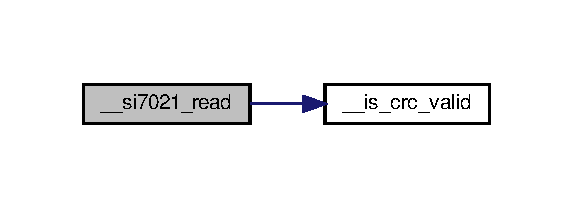
\includegraphics[width=275pt]{si7021_8h_a06d36b1f00051ed948cf054b4700d1ec_cgraph}
\end{center}
\end{figure}
\mbox{\Hypertarget{si7021_8h_a91041d121bd0dff34dc9383479286e2d}\label{si7021_8h_a91041d121bd0dff34dc9383479286e2d}} 
\index{si7021.\+h@{si7021.\+h}!\+\_\+\+\_\+si7021\+\_\+read\+\_\+user\+\_\+register@{\+\_\+\+\_\+si7021\+\_\+read\+\_\+user\+\_\+register}}
\index{\+\_\+\+\_\+si7021\+\_\+read\+\_\+user\+\_\+register@{\+\_\+\+\_\+si7021\+\_\+read\+\_\+user\+\_\+register}!si7021.\+h@{si7021.\+h}}
\subsubsection{\texorpdfstring{\+\_\+\+\_\+si7021\+\_\+read\+\_\+user\+\_\+register()}{\_\_si7021\_read\_user\_register()}}
{\footnotesize\ttfamily uint8\+\_\+t \+\_\+\+\_\+si7021\+\_\+read\+\_\+user\+\_\+register (\begin{DoxyParamCaption}{ }\end{DoxyParamCaption})}



Read R\+H/T user register 1 from sensor. 

\begin{DoxyNote}{Note}
Internal use only 
\end{DoxyNote}
\begin{DoxyReturn}{Returns}

\begin{DoxyItemize}
\item 8bit (unit8\+\_\+t) value, contain content of user R\+H/T register
\item 0 if failed to read 
\end{DoxyItemize}
\end{DoxyReturn}


Definition at line 193 of file si7021.\+c.



References S\+I7021\+\_\+\+A\+D\+DR, si7021\+\_\+config\+\_\+t\+::si7021\+\_\+port, and S\+I7021\+\_\+\+R\+E\+A\+D\+R\+H\+T\+\_\+\+R\+E\+G\+\_\+\+C\+MD.



Referenced by si7021\+\_\+get\+\_\+heater\+\_\+status(), si7021\+\_\+get\+\_\+resolution(), si7021\+\_\+read\+\_\+vdd\+\_\+status(), si7021\+\_\+set\+\_\+heater\+\_\+status(), and si7021\+\_\+set\+\_\+resolution().

\mbox{\Hypertarget{si7021_8h_ab01f45ffce7fdfa1f150f4b3f15c4e33}\label{si7021_8h_ab01f45ffce7fdfa1f150f4b3f15c4e33}} 
\index{si7021.\+h@{si7021.\+h}!\+\_\+\+\_\+si7021\+\_\+write\+\_\+user\+\_\+register@{\+\_\+\+\_\+si7021\+\_\+write\+\_\+user\+\_\+register}}
\index{\+\_\+\+\_\+si7021\+\_\+write\+\_\+user\+\_\+register@{\+\_\+\+\_\+si7021\+\_\+write\+\_\+user\+\_\+register}!si7021.\+h@{si7021.\+h}}
\subsubsection{\texorpdfstring{\+\_\+\+\_\+si7021\+\_\+write\+\_\+user\+\_\+register()}{\_\_si7021\_write\_user\_register()}}
{\footnotesize\ttfamily \hyperlink{si7021_8h_aeec681879f00b18fe17bddc989b9582d}{si7021\+\_\+err\+\_\+t} \+\_\+\+\_\+si7021\+\_\+write\+\_\+user\+\_\+register (\begin{DoxyParamCaption}\item[{uint8\+\_\+t}]{value }\end{DoxyParamCaption})}



Write value to R\+H/T user register 1. 

\begin{DoxyNote}{Note}
Internal use only 
\end{DoxyNote}

\begin{DoxyParams}{Parameters}
{\em value} & Value to write to register \\
\hline
\end{DoxyParams}
\begin{DoxyReturn}{Returns}

\begin{DoxyItemize}
\item \hyperlink{group__SI7021__RT__VALUE_ga04cef12730209bc72277b64111308b42}{S\+I7021\+\_\+\+E\+R\+R\+\_\+\+OK} Success
\item \hyperlink{group__SI7021__RT__VALUE_gad1c1ac433562f82e632c21f92c0fd4a3}{S\+I7021\+\_\+\+E\+R\+R\+\_\+\+I\+N\+V\+A\+L\+I\+D\+\_\+\+A\+RG} Invalid arguments
\item \hyperlink{group__SI7021__RT__VALUE_ga7cc0cccf705f1f1807d09abc3d1bea14}{S\+I7021\+\_\+\+E\+R\+R\+\_\+\+F\+A\+IL} Failed to write
\item \hyperlink{group__SI7021__RT__VALUE_gadf36521836ea146264b0db90fd02fb45}{S\+I7021\+\_\+\+E\+R\+R\+\_\+\+I\+N\+V\+A\+L\+I\+D\+\_\+\+S\+T\+A\+TE} Sensor is in invalid state
\item \hyperlink{group__SI7021__RT__VALUE_gaf3c553ace8f63aa562e2263c47a1b5ed}{S\+I7021\+\_\+\+E\+R\+R\+\_\+\+T\+I\+M\+E\+O\+UT} Timed out communicating with sensor 
\end{DoxyItemize}
\end{DoxyReturn}


Definition at line 240 of file si7021.\+c.



References S\+I7021\+\_\+\+A\+D\+DR, S\+I7021\+\_\+\+E\+R\+R\+\_\+\+F\+A\+IL, S\+I7021\+\_\+\+E\+R\+R\+\_\+\+I\+N\+V\+A\+L\+I\+D\+\_\+\+A\+RG, S\+I7021\+\_\+\+E\+R\+R\+\_\+\+I\+N\+V\+A\+L\+I\+D\+\_\+\+S\+T\+A\+TE, S\+I7021\+\_\+\+E\+R\+R\+\_\+\+OK, S\+I7021\+\_\+\+E\+R\+R\+\_\+\+T\+I\+M\+E\+O\+UT, si7021\+\_\+config\+\_\+t\+::si7021\+\_\+port, and S\+I7021\+\_\+\+W\+R\+I\+T\+E\+R\+H\+T\+\_\+\+R\+E\+G\+\_\+\+C\+MD.



Referenced by si7021\+\_\+set\+\_\+heater\+\_\+status(), and si7021\+\_\+set\+\_\+resolution().

\mbox{\Hypertarget{si7021_8h_ab0d521e94113c17457f8898e37410009}\label{si7021_8h_ab0d521e94113c17457f8898e37410009}} 
\index{si7021.\+h@{si7021.\+h}!get\+\_\+electronic\+\_\+id@{get\+\_\+electronic\+\_\+id}}
\index{get\+\_\+electronic\+\_\+id@{get\+\_\+electronic\+\_\+id}!si7021.\+h@{si7021.\+h}}
\subsubsection{\texorpdfstring{get\+\_\+electronic\+\_\+id()}{get\_electronic\_id()}}
{\footnotesize\ttfamily uint64\+\_\+t get\+\_\+electronic\+\_\+id (\begin{DoxyParamCaption}{ }\end{DoxyParamCaption})}



Get sensor electronic id. 

\begin{DoxyReturn}{Returns}
64bit (uint64\+\_\+t) value contain sensor electronic id 
\end{DoxyReturn}
\begin{DoxyNote}{Note}
if error happen, return 0x\+F\+F\+F\+F\+F\+F\+F\+F\+F\+F\+F\+F\+F\+F\+FF 
\end{DoxyNote}


Definition at line 370 of file si7021.\+c.



References S\+I7021\+\_\+\+A\+D\+DR, S\+I7021\+\_\+\+I\+D1\+\_\+\+C\+MD, S\+I7021\+\_\+\+I\+D2\+\_\+\+C\+MD, and si7021\+\_\+config\+\_\+t\+::si7021\+\_\+port.

\mbox{\Hypertarget{si7021_8h_a17554408b2bda4f9219d479946e30fbb}\label{si7021_8h_a17554408b2bda4f9219d479946e30fbb}} 
\index{si7021.\+h@{si7021.\+h}!si7021\+\_\+check\+\_\+availability@{si7021\+\_\+check\+\_\+availability}}
\index{si7021\+\_\+check\+\_\+availability@{si7021\+\_\+check\+\_\+availability}!si7021.\+h@{si7021.\+h}}
\subsubsection{\texorpdfstring{si7021\+\_\+check\+\_\+availability()}{si7021\_check\_availability()}}
{\footnotesize\ttfamily \hyperlink{si7021_8h_aeec681879f00b18fe17bddc989b9582d}{si7021\+\_\+err\+\_\+t} si7021\+\_\+check\+\_\+availability (\begin{DoxyParamCaption}{ }\end{DoxyParamCaption})}



Check the availability of sensor. 

\begin{DoxyReturn}{Returns}

\begin{DoxyItemize}
\item \hyperlink{group__SI7021__RT__VALUE_ga04cef12730209bc72277b64111308b42}{S\+I7021\+\_\+\+E\+R\+R\+\_\+\+OK} Sensor detected and available
\item \hyperlink{group__SI7021__RT__VALUE_ga277249c1e2c9ac97e4bec42c79ad4e49}{S\+I7021\+\_\+\+E\+R\+R\+\_\+\+N\+O\+T\+F\+O\+U\+ND} Sensor missing and/or not available 
\end{DoxyItemize}
\end{DoxyReturn}


Definition at line 71 of file si7021.\+c.



References S\+I7021\+\_\+\+A\+D\+DR, S\+I7021\+\_\+\+E\+R\+R\+\_\+\+N\+O\+T\+F\+O\+U\+ND, S\+I7021\+\_\+\+E\+R\+R\+\_\+\+OK, and si7021\+\_\+config\+\_\+t\+::si7021\+\_\+port.



Referenced by si7021\+\_\+init().

\mbox{\Hypertarget{si7021_8h_ad85d7885ebbb87e1ac1f12b78a6c0af7}\label{si7021_8h_ad85d7885ebbb87e1ac1f12b78a6c0af7}} 
\index{si7021.\+h@{si7021.\+h}!si7021\+\_\+get\+\_\+heater\+\_\+register@{si7021\+\_\+get\+\_\+heater\+\_\+register}}
\index{si7021\+\_\+get\+\_\+heater\+\_\+register@{si7021\+\_\+get\+\_\+heater\+\_\+register}!si7021.\+h@{si7021.\+h}}
\subsubsection{\texorpdfstring{si7021\+\_\+get\+\_\+heater\+\_\+register()}{si7021\_get\_heater\_register()}}
{\footnotesize\ttfamily uint8\+\_\+t si7021\+\_\+get\+\_\+heater\+\_\+register (\begin{DoxyParamCaption}{ }\end{DoxyParamCaption})}



Read heater register. 

\begin{DoxyReturn}{Returns}
8bit (uint8\+\_\+t) value contain content of heater register
\begin{DoxyItemize}
\item 0xF\+: 94.\+20mA
\item 0x8\+: 51.\+96mA
\item 0x4\+: 27.\+39mA
\item 0x2\+: 15.\+24mA
\item 0x1\+: 9.\+18mA
\item 0x0\+: 3.\+09mA 
\end{DoxyItemize}
\end{DoxyReturn}


Definition at line 311 of file si7021.\+c.



References S\+I7021\+\_\+\+A\+D\+DR, si7021\+\_\+config\+\_\+t\+::si7021\+\_\+port, and S\+I7021\+\_\+\+R\+E\+A\+D\+H\+E\+A\+T\+E\+R\+\_\+\+R\+E\+G\+\_\+\+C\+MD.

\mbox{\Hypertarget{si7021_8h_a6ec069cec3b96b638c8f0426aca309b2}\label{si7021_8h_a6ec069cec3b96b638c8f0426aca309b2}} 
\index{si7021.\+h@{si7021.\+h}!si7021\+\_\+get\+\_\+heater\+\_\+status@{si7021\+\_\+get\+\_\+heater\+\_\+status}}
\index{si7021\+\_\+get\+\_\+heater\+\_\+status@{si7021\+\_\+get\+\_\+heater\+\_\+status}!si7021.\+h@{si7021.\+h}}
\subsubsection{\texorpdfstring{si7021\+\_\+get\+\_\+heater\+\_\+status()}{si7021\_get\_heater\_status()}}
{\footnotesize\ttfamily uint8\+\_\+t si7021\+\_\+get\+\_\+heater\+\_\+status (\begin{DoxyParamCaption}{ }\end{DoxyParamCaption})}



Check sensors heater status. 

\begin{DoxyReturn}{Returns}
8bit (uint8\+\_\+t) value
\begin{DoxyItemize}
\item \hyperlink{si7021_8h_af209481235e9da082e1447dc34478651}{S\+I7021\+\_\+\+H\+E\+A\+T\+E\+R\+\_\+\+ON} H\+E\+A\+T\+ER is ON
\item \hyperlink{si7021_8h_a7b49e55ef2f682cfe12cd29a09283e68}{S\+I7021\+\_\+\+H\+E\+A\+T\+E\+R\+\_\+\+O\+FF} H\+E\+A\+T\+ER is O\+FF 
\end{DoxyItemize}
\end{DoxyReturn}


Definition at line 304 of file si7021.\+c.



References \+\_\+\+\_\+si7021\+\_\+read\+\_\+user\+\_\+register(), S\+I7021\+\_\+\+H\+E\+A\+T\+E\+R\+\_\+\+O\+FF, and S\+I7021\+\_\+\+H\+E\+A\+T\+E\+R\+\_\+\+ON.

Here is the call graph for this function\+:\nopagebreak
\begin{figure}[H]
\begin{center}
\leavevmode
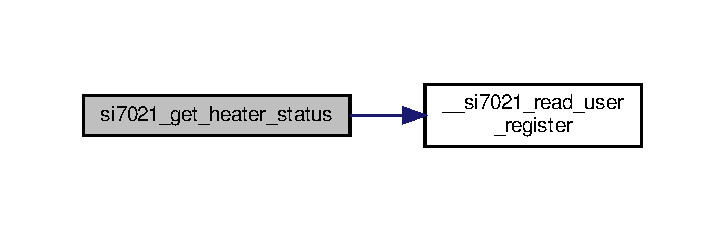
\includegraphics[width=348pt]{si7021_8h_a6ec069cec3b96b638c8f0426aca309b2_cgraph}
\end{center}
\end{figure}
\mbox{\Hypertarget{si7021_8h_a7347c3be7bfb07b492e4cbed1cdbcfb9}\label{si7021_8h_a7347c3be7bfb07b492e4cbed1cdbcfb9}} 
\index{si7021.\+h@{si7021.\+h}!si7021\+\_\+get\+\_\+resolution@{si7021\+\_\+get\+\_\+resolution}}
\index{si7021\+\_\+get\+\_\+resolution@{si7021\+\_\+get\+\_\+resolution}!si7021.\+h@{si7021.\+h}}
\subsubsection{\texorpdfstring{si7021\+\_\+get\+\_\+resolution()}{si7021\_get\_resolution()}}
{\footnotesize\ttfamily \hyperlink{si7021_8h_ad2e0aa498b8faee91d8da4930f61625e}{S\+I7021\+\_\+\+R\+E\+S\+O\+L\+U\+T\+I\+ON} si7021\+\_\+get\+\_\+resolution (\begin{DoxyParamCaption}{ }\end{DoxyParamCaption})}



Get current resolution of sensor. 

\begin{DoxyReturn}{Returns}

\begin{DoxyItemize}
\item 0x00\+: 12bit RH resolution, 14bit temperature resolution
\item 0x01\+: 8bit RH resolution, 12bit temperature resolution
\item 0x80\+: 10bit RH resolution, 13bit temperature resolution
\item 0x81\+: 11bit RH resolution, 11bit temperature resolution 
\end{DoxyItemize}
\end{DoxyReturn}


Definition at line 221 of file si7021.\+c.



References \+\_\+\+\_\+si7021\+\_\+read\+\_\+user\+\_\+register().

Here is the call graph for this function\+:\nopagebreak
\begin{figure}[H]
\begin{center}
\leavevmode
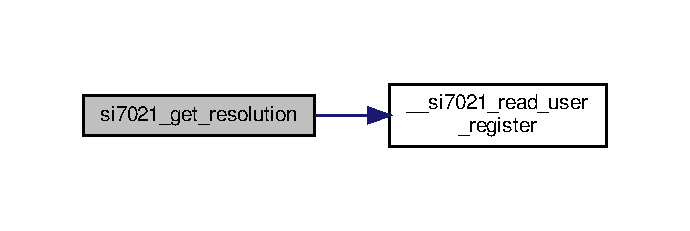
\includegraphics[width=331pt]{si7021_8h_a7347c3be7bfb07b492e4cbed1cdbcfb9_cgraph}
\end{center}
\end{figure}
\mbox{\Hypertarget{si7021_8h_a82f9c8e22626638e47729098f8493c1f}\label{si7021_8h_a82f9c8e22626638e47729098f8493c1f}} 
\index{si7021.\+h@{si7021.\+h}!si7021\+\_\+init@{si7021\+\_\+init}}
\index{si7021\+\_\+init@{si7021\+\_\+init}!si7021.\+h@{si7021.\+h}}
\subsubsection{\texorpdfstring{si7021\+\_\+init()}{si7021\_init()}}
{\footnotesize\ttfamily \hyperlink{si7021_8h_aeec681879f00b18fe17bddc989b9582d}{si7021\+\_\+err\+\_\+t} si7021\+\_\+init (\begin{DoxyParamCaption}\item[{\hyperlink{structsi7021__config__t}{si7021\+\_\+config\+\_\+t} $\ast$}]{config }\end{DoxyParamCaption})}



Initialize S\+I7021 sensor. 


\begin{DoxyParams}{Parameters}
{\em config} & \hyperlink{structsi7021__config__t}{si7021\+\_\+config\+\_\+t} struct that contain sensors information and configuration \\
\hline
\end{DoxyParams}
\begin{DoxyReturn}{Returns}

\begin{DoxyItemize}
\item \hyperlink{group__SI7021__RT__VALUE_ga04cef12730209bc72277b64111308b42}{S\+I7021\+\_\+\+E\+R\+R\+\_\+\+OK} Success.
\item \hyperlink{group__SI7021__RT__VALUE_ga0abfa8d0b3297244d470fcdbce8e39da}{S\+I7021\+\_\+\+E\+R\+R\+\_\+\+C\+O\+N\+F\+IG} Failed to configure I2C parameter, forwarded return from \hyperlink{si7021_8h_a339f08aa1ed1d74c2c12fd904ea4e28c}{\+\_\+\+\_\+si7021\+\_\+param\+\_\+config}(\hyperlink{structsi7021__config__t}{si7021\+\_\+config\+\_\+t} $\ast$config)
\item \hyperlink{group__SI7021__RT__VALUE_ga1a536c4aff63acd66547e006b587841b}{S\+I7021\+\_\+\+E\+R\+R\+\_\+\+I\+N\+S\+T\+A\+LL} Failed to configure I2C Driver, forwarded return from \hyperlink{si7021_8h_a814069add0f4e59b5f254732d37637bf}{\+\_\+\+\_\+si7021\+\_\+driver\+\_\+config}(\hyperlink{structsi7021__config__t}{si7021\+\_\+config\+\_\+t} $\ast$config)
\item \hyperlink{group__SI7021__RT__VALUE_ga277249c1e2c9ac97e4bec42c79ad4e49}{S\+I7021\+\_\+\+E\+R\+R\+\_\+\+N\+O\+T\+F\+O\+U\+ND} Sensor missing and/or not available, forwarded return from \hyperlink{si7021_8h_a17554408b2bda4f9219d479946e30fbb}{si7021\+\_\+check\+\_\+availability()} 
\end{DoxyItemize}
\end{DoxyReturn}


Definition at line 34 of file si7021.\+c.



References \+\_\+\+\_\+si7021\+\_\+driver\+\_\+config(), \+\_\+\+\_\+si7021\+\_\+param\+\_\+config(), si7021\+\_\+check\+\_\+availability(), and S\+I7021\+\_\+\+E\+R\+R\+\_\+\+OK.

Here is the call graph for this function\+:\nopagebreak
\begin{figure}[H]
\begin{center}
\leavevmode
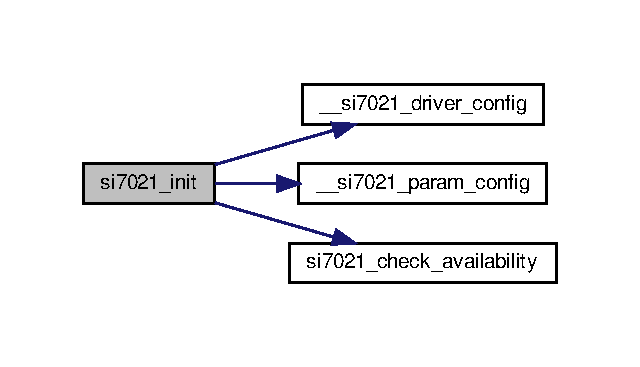
\includegraphics[width=307pt]{si7021_8h_a82f9c8e22626638e47729098f8493c1f_cgraph}
\end{center}
\end{figure}
\mbox{\Hypertarget{si7021_8h_a1e1e3955782fa3079544f048d42ad88e}\label{si7021_8h_a1e1e3955782fa3079544f048d42ad88e}} 
\index{si7021.\+h@{si7021.\+h}!si7021\+\_\+read\+\_\+firmware\+\_\+rev@{si7021\+\_\+read\+\_\+firmware\+\_\+rev}}
\index{si7021\+\_\+read\+\_\+firmware\+\_\+rev@{si7021\+\_\+read\+\_\+firmware\+\_\+rev}!si7021.\+h@{si7021.\+h}}
\subsubsection{\texorpdfstring{si7021\+\_\+read\+\_\+firmware\+\_\+rev()}{si7021\_read\_firmware\_rev()}}
{\footnotesize\ttfamily uint8\+\_\+t si7021\+\_\+read\+\_\+firmware\+\_\+rev (\begin{DoxyParamCaption}{ }\end{DoxyParamCaption})}



Read sensor firmware revision. 

\begin{DoxyReturn}{Returns}
8bit (uint8\+\_\+t) value contain sensor firmware revision
\begin{DoxyItemize}
\item 0x\+FF\+: Firmware version 1.\+0
\item 0x20\+: Firmware version 2.\+0 
\end{DoxyItemize}
\end{DoxyReturn}


Definition at line 269 of file si7021.\+c.



References S\+I7021\+\_\+\+A\+D\+DR, S\+I7021\+\_\+\+F\+I\+R\+M\+V\+E\+R\+S\+\_\+\+C\+MD, and si7021\+\_\+config\+\_\+t\+::si7021\+\_\+port.

\mbox{\Hypertarget{si7021_8h_afebf7dfa4b71f1d0848955edf97a8156}\label{si7021_8h_afebf7dfa4b71f1d0848955edf97a8156}} 
\index{si7021.\+h@{si7021.\+h}!si7021\+\_\+read\+\_\+humidity@{si7021\+\_\+read\+\_\+humidity}}
\index{si7021\+\_\+read\+\_\+humidity@{si7021\+\_\+read\+\_\+humidity}!si7021.\+h@{si7021.\+h}}
\subsubsection{\texorpdfstring{si7021\+\_\+read\+\_\+humidity()}{si7021\_read\_humidity()}}
{\footnotesize\ttfamily float si7021\+\_\+read\+\_\+humidity (\begin{DoxyParamCaption}{ }\end{DoxyParamCaption})}



Read \href{https://en.wikipedia.org/wiki/Relative_humidity}{\tt Relative Humidity} value from sensor. 

\begin{DoxyReturn}{Returns}
float value, \href{https://en.wikipedia.org/wiki/Relative_humidity}{\tt Relative Humidity} in percentage 
\end{DoxyReturn}


Definition at line 94 of file si7021.\+c.



References \+\_\+\+\_\+si7021\+\_\+read(), and S\+I7021\+\_\+\+M\+E\+A\+S\+R\+H\+\_\+\+N\+O\+H\+O\+L\+D\+\_\+\+C\+MD.

Here is the call graph for this function\+:\nopagebreak
\begin{figure}[H]
\begin{center}
\leavevmode
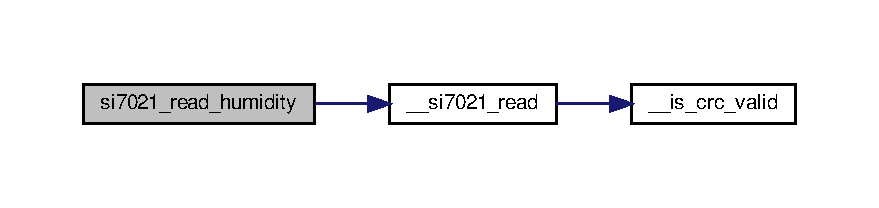
\includegraphics[width=350pt]{si7021_8h_afebf7dfa4b71f1d0848955edf97a8156_cgraph}
\end{center}
\end{figure}
\mbox{\Hypertarget{si7021_8h_aac2b7c97826cdeb499ac224a8120fee2}\label{si7021_8h_aac2b7c97826cdeb499ac224a8120fee2}} 
\index{si7021.\+h@{si7021.\+h}!si7021\+\_\+read\+\_\+temperature@{si7021\+\_\+read\+\_\+temperature}}
\index{si7021\+\_\+read\+\_\+temperature@{si7021\+\_\+read\+\_\+temperature}!si7021.\+h@{si7021.\+h}}
\subsubsection{\texorpdfstring{si7021\+\_\+read\+\_\+temperature()}{si7021\_read\_temperature()}}
{\footnotesize\ttfamily float si7021\+\_\+read\+\_\+temperature (\begin{DoxyParamCaption}{ }\end{DoxyParamCaption})}



Read temperature value from sensor. 

\begin{DoxyReturn}{Returns}
float value, temperature in \href{https://en.wikipedia.org/wiki/Celsius}{\tt Celsius} 
\end{DoxyReturn}


Definition at line 86 of file si7021.\+c.



References \+\_\+\+\_\+si7021\+\_\+read(), and S\+I7021\+\_\+\+M\+E\+A\+S\+T\+E\+M\+P\+\_\+\+N\+O\+H\+O\+L\+D\+\_\+\+C\+MD.

Here is the call graph for this function\+:\nopagebreak
\begin{figure}[H]
\begin{center}
\leavevmode
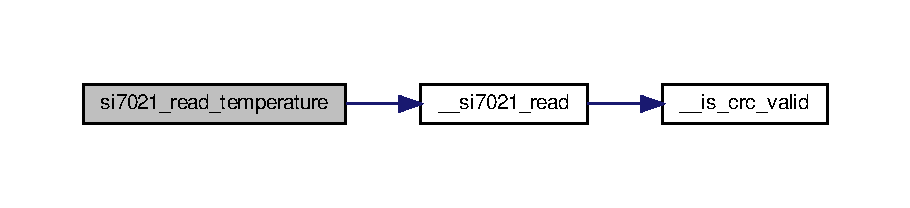
\includegraphics[width=350pt]{si7021_8h_aac2b7c97826cdeb499ac224a8120fee2_cgraph}
\end{center}
\end{figure}
\mbox{\Hypertarget{si7021_8h_a5b42332bda6837327d02700bbaca7060}\label{si7021_8h_a5b42332bda6837327d02700bbaca7060}} 
\index{si7021.\+h@{si7021.\+h}!si7021\+\_\+read\+\_\+vdd\+\_\+status@{si7021\+\_\+read\+\_\+vdd\+\_\+status}}
\index{si7021\+\_\+read\+\_\+vdd\+\_\+status@{si7021\+\_\+read\+\_\+vdd\+\_\+status}!si7021.\+h@{si7021.\+h}}
\subsubsection{\texorpdfstring{si7021\+\_\+read\+\_\+vdd\+\_\+status()}{si7021\_read\_vdd\_status()}}
{\footnotesize\ttfamily \hyperlink{si7021_8h_ae8747642c3a83dd9ae9ae0333b84f9f3}{S\+I7021\+\_\+\+V\+D\+D\+\_\+\+S\+T\+A\+T\+US} si7021\+\_\+read\+\_\+vdd\+\_\+status (\begin{DoxyParamCaption}{ }\end{DoxyParamCaption})}



Check sensors V\+DD. 

\begin{DoxyReturn}{Returns}
8bit (uint8\+\_\+t) value
\begin{DoxyItemize}
\item \hyperlink{si7021_8h_ae8747642c3a83dd9ae9ae0333b84f9f3acdfe83b75cad583ca9ee2997322174ea}{S\+I7021\+\_\+\+V\+D\+D\+\_\+\+OK} V\+DD is OK
\item \hyperlink{si7021_8h_ae8747642c3a83dd9ae9ae0333b84f9f3a1ad64fa668e0c9b079a23971c4bb1505}{S\+I7021\+\_\+\+V\+D\+D\+\_\+\+L\+OW} V\+DD is L\+OW 
\end{DoxyItemize}
\end{DoxyReturn}
\begin{DoxyNote}{Note}
Consider changing power supply when V\+DD is L\+OW, sensors may not work correctly 
\end{DoxyNote}


Definition at line 297 of file si7021.\+c.



References \+\_\+\+\_\+si7021\+\_\+read\+\_\+user\+\_\+register(), S\+I7021\+\_\+\+V\+D\+D\+\_\+\+L\+OW, and S\+I7021\+\_\+\+V\+D\+D\+\_\+\+OK.

Here is the call graph for this function\+:\nopagebreak
\begin{figure}[H]
\begin{center}
\leavevmode
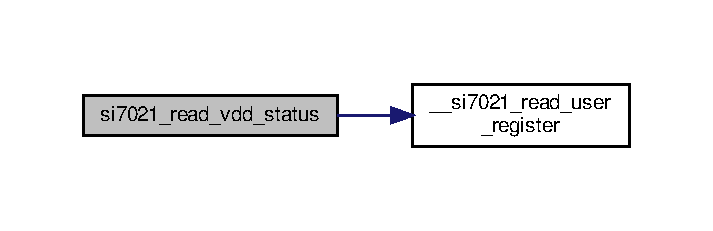
\includegraphics[width=342pt]{si7021_8h_a5b42332bda6837327d02700bbaca7060_cgraph}
\end{center}
\end{figure}
\mbox{\Hypertarget{si7021_8h_ab4db1385ee975ed53c1b4cb8b2f82da7}\label{si7021_8h_ab4db1385ee975ed53c1b4cb8b2f82da7}} 
\index{si7021.\+h@{si7021.\+h}!si7021\+\_\+set\+\_\+heater\+\_\+register@{si7021\+\_\+set\+\_\+heater\+\_\+register}}
\index{si7021\+\_\+set\+\_\+heater\+\_\+register@{si7021\+\_\+set\+\_\+heater\+\_\+register}!si7021.\+h@{si7021.\+h}}
\subsubsection{\texorpdfstring{si7021\+\_\+set\+\_\+heater\+\_\+register()}{si7021\_set\_heater\_register()}}
{\footnotesize\ttfamily \hyperlink{si7021_8h_aeec681879f00b18fe17bddc989b9582d}{si7021\+\_\+err\+\_\+t} si7021\+\_\+set\+\_\+heater\+\_\+register (\begin{DoxyParamCaption}\item[{uint8\+\_\+t}]{value }\end{DoxyParamCaption})}



Set heater register. 


\begin{DoxyParams}{Parameters}
{\em value} & 8bit (uint8\+\_\+t) value that will be written to heater register
\begin{DoxyItemize}
\item 0xF\+: 94.\+20mA
\item 0x8\+: 51.\+96mA
\item 0x4\+: 27.\+39mA
\item 0x2\+: 15.\+24mA
\item 0x1\+: 9.\+18mA
\item 0x0\+: 3.\+09mA 
\end{DoxyItemize}\\
\hline
\end{DoxyParams}


Definition at line 338 of file si7021.\+c.



References S\+I7021\+\_\+\+A\+D\+DR, S\+I7021\+\_\+\+E\+R\+R\+\_\+\+F\+A\+IL, S\+I7021\+\_\+\+E\+R\+R\+\_\+\+I\+N\+V\+A\+L\+I\+D\+\_\+\+A\+RG, S\+I7021\+\_\+\+E\+R\+R\+\_\+\+I\+N\+V\+A\+L\+I\+D\+\_\+\+S\+T\+A\+TE, S\+I7021\+\_\+\+E\+R\+R\+\_\+\+OK, S\+I7021\+\_\+\+E\+R\+R\+\_\+\+T\+I\+M\+E\+O\+UT, si7021\+\_\+config\+\_\+t\+::si7021\+\_\+port, and S\+I7021\+\_\+\+W\+R\+I\+T\+E\+H\+E\+A\+T\+E\+R\+\_\+\+R\+E\+G\+\_\+\+C\+MD.

\mbox{\Hypertarget{si7021_8h_a65fe3b1e33bdbebf8df2c8d51bbbf675}\label{si7021_8h_a65fe3b1e33bdbebf8df2c8d51bbbf675}} 
\index{si7021.\+h@{si7021.\+h}!si7021\+\_\+set\+\_\+heater\+\_\+status@{si7021\+\_\+set\+\_\+heater\+\_\+status}}
\index{si7021\+\_\+set\+\_\+heater\+\_\+status@{si7021\+\_\+set\+\_\+heater\+\_\+status}!si7021.\+h@{si7021.\+h}}
\subsubsection{\texorpdfstring{si7021\+\_\+set\+\_\+heater\+\_\+status()}{si7021\_set\_heater\_status()}}
{\footnotesize\ttfamily \hyperlink{si7021_8h_aeec681879f00b18fe17bddc989b9582d}{si7021\+\_\+err\+\_\+t} si7021\+\_\+set\+\_\+heater\+\_\+status (\begin{DoxyParamCaption}\item[{uint8\+\_\+t}]{value }\end{DoxyParamCaption})}



Set heater status. 


\begin{DoxyParams}{Parameters}
{\em value} & Heater status will be set to this
\begin{DoxyItemize}
\item \hyperlink{si7021_8h_af209481235e9da082e1447dc34478651}{S\+I7021\+\_\+\+H\+E\+A\+T\+E\+R\+\_\+\+ON}\+: H\+E\+A\+T\+ER will be turn on
\item \hyperlink{si7021_8h_a7b49e55ef2f682cfe12cd29a09283e68}{S\+I7021\+\_\+\+H\+E\+A\+T\+E\+R\+\_\+\+O\+FF}\+: H\+E\+A\+T\+ER will be turn off 
\end{DoxyItemize}\\
\hline
\end{DoxyParams}


Definition at line 361 of file si7021.\+c.



References \+\_\+\+\_\+si7021\+\_\+read\+\_\+user\+\_\+register(), \+\_\+\+\_\+si7021\+\_\+write\+\_\+user\+\_\+register(), S\+I7021\+\_\+\+H\+E\+A\+T\+E\+R\+\_\+\+O\+FF, and S\+I7021\+\_\+\+H\+E\+A\+T\+E\+R\+\_\+\+ON.

Here is the call graph for this function\+:\nopagebreak
\begin{figure}[H]
\begin{center}
\leavevmode
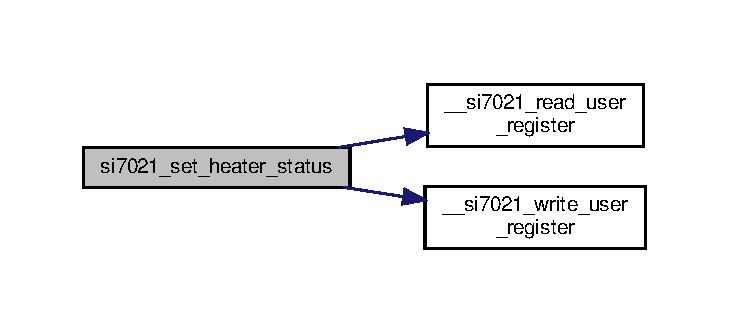
\includegraphics[width=350pt]{si7021_8h_a65fe3b1e33bdbebf8df2c8d51bbbf675_cgraph}
\end{center}
\end{figure}
\mbox{\Hypertarget{si7021_8h_afd590ce231e3b83309411c505af7e169}\label{si7021_8h_afd590ce231e3b83309411c505af7e169}} 
\index{si7021.\+h@{si7021.\+h}!si7021\+\_\+set\+\_\+resolution@{si7021\+\_\+set\+\_\+resolution}}
\index{si7021\+\_\+set\+\_\+resolution@{si7021\+\_\+set\+\_\+resolution}!si7021.\+h@{si7021.\+h}}
\subsubsection{\texorpdfstring{si7021\+\_\+set\+\_\+resolution()}{si7021\_set\_resolution()}}
{\footnotesize\ttfamily \hyperlink{si7021_8h_aeec681879f00b18fe17bddc989b9582d}{si7021\+\_\+err\+\_\+t} si7021\+\_\+set\+\_\+resolution (\begin{DoxyParamCaption}\item[{\hyperlink{si7021_8h_ad2e0aa498b8faee91d8da4930f61625e}{S\+I7021\+\_\+\+R\+E\+S\+O\+L\+U\+T\+I\+ON}}]{resolution }\end{DoxyParamCaption})}



Set the sensors resolution. 


\begin{DoxyParams}{Parameters}
{\em resolution} & The resolution will be set \\
\hline
\end{DoxyParams}
\begin{DoxyReturn}{Returns}

\begin{DoxyItemize}
\item \hyperlink{group__SI7021__RT__VALUE_ga04cef12730209bc72277b64111308b42}{S\+I7021\+\_\+\+E\+R\+R\+\_\+\+OK} Success
\item \hyperlink{group__SI7021__RT__VALUE_gad1c1ac433562f82e632c21f92c0fd4a3}{S\+I7021\+\_\+\+E\+R\+R\+\_\+\+I\+N\+V\+A\+L\+I\+D\+\_\+\+A\+RG} Invalid arguments
\item \hyperlink{group__SI7021__RT__VALUE_ga7cc0cccf705f1f1807d09abc3d1bea14}{S\+I7021\+\_\+\+E\+R\+R\+\_\+\+F\+A\+IL} Failed to write
\item \hyperlink{group__SI7021__RT__VALUE_gadf36521836ea146264b0db90fd02fb45}{S\+I7021\+\_\+\+E\+R\+R\+\_\+\+I\+N\+V\+A\+L\+I\+D\+\_\+\+S\+T\+A\+TE} Sensor is in invalid state
\item \hyperlink{group__SI7021__RT__VALUE_gaf3c553ace8f63aa562e2263c47a1b5ed}{S\+I7021\+\_\+\+E\+R\+R\+\_\+\+T\+I\+M\+E\+O\+UT} Timed out communicating with sensor 
\end{DoxyItemize}
\end{DoxyReturn}


Definition at line 225 of file si7021.\+c.



References \+\_\+\+\_\+si7021\+\_\+read\+\_\+user\+\_\+register(), and \+\_\+\+\_\+si7021\+\_\+write\+\_\+user\+\_\+register().

Here is the call graph for this function\+:\nopagebreak
\begin{figure}[H]
\begin{center}
\leavevmode
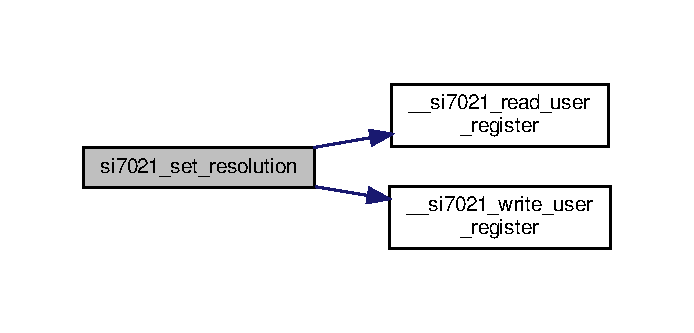
\includegraphics[width=333pt]{si7021_8h_afd590ce231e3b83309411c505af7e169_cgraph}
\end{center}
\end{figure}
\mbox{\Hypertarget{si7021_8h_a7800e376fe6c29d695e3dd36ad28a1e9}\label{si7021_8h_a7800e376fe6c29d695e3dd36ad28a1e9}} 
\index{si7021.\+h@{si7021.\+h}!si7021\+\_\+soft\+\_\+reset@{si7021\+\_\+soft\+\_\+reset}}
\index{si7021\+\_\+soft\+\_\+reset@{si7021\+\_\+soft\+\_\+reset}!si7021.\+h@{si7021.\+h}}
\subsubsection{\texorpdfstring{si7021\+\_\+soft\+\_\+reset()}{si7021\_soft\_reset()}}
{\footnotesize\ttfamily \hyperlink{si7021_8h_aeec681879f00b18fe17bddc989b9582d}{si7021\+\_\+err\+\_\+t} si7021\+\_\+soft\+\_\+reset (\begin{DoxyParamCaption}{ }\end{DoxyParamCaption})}



Reset the sensor. 

\begin{DoxyNote}{Note}
Reset will erase all setting, register... 
\end{DoxyNote}
\begin{DoxyReturn}{Returns}

\begin{DoxyItemize}
\item \hyperlink{group__SI7021__RT__VALUE_ga04cef12730209bc72277b64111308b42}{S\+I7021\+\_\+\+E\+R\+R\+\_\+\+OK} Success
\item \hyperlink{group__SI7021__RT__VALUE_gaf3c553ace8f63aa562e2263c47a1b5ed}{S\+I7021\+\_\+\+E\+R\+R\+\_\+\+T\+I\+M\+E\+O\+UT} Timed out communicating with sensor
\item \hyperlink{group__SI7021__RT__VALUE_gadf36521836ea146264b0db90fd02fb45}{S\+I7021\+\_\+\+E\+R\+R\+\_\+\+I\+N\+V\+A\+L\+I\+D\+\_\+\+S\+T\+A\+TE} Sensor is in invalid state
\item \hyperlink{group__SI7021__RT__VALUE_ga7cc0cccf705f1f1807d09abc3d1bea14}{S\+I7021\+\_\+\+E\+R\+R\+\_\+\+F\+A\+IL} Failed
\item \hyperlink{group__SI7021__RT__VALUE_gad1c1ac433562f82e632c21f92c0fd4a3}{S\+I7021\+\_\+\+E\+R\+R\+\_\+\+I\+N\+V\+A\+L\+I\+D\+\_\+\+A\+RG} Invalid arguments 
\end{DoxyItemize}
\end{DoxyReturn}


Definition at line 167 of file si7021.\+c.



References S\+I7021\+\_\+\+A\+D\+DR, S\+I7021\+\_\+\+E\+R\+R\+\_\+\+F\+A\+IL, S\+I7021\+\_\+\+E\+R\+R\+\_\+\+I\+N\+V\+A\+L\+I\+D\+\_\+\+A\+RG, S\+I7021\+\_\+\+E\+R\+R\+\_\+\+I\+N\+V\+A\+L\+I\+D\+\_\+\+S\+T\+A\+TE, S\+I7021\+\_\+\+E\+R\+R\+\_\+\+OK, S\+I7021\+\_\+\+E\+R\+R\+\_\+\+T\+I\+M\+E\+O\+UT, si7021\+\_\+config\+\_\+t\+::si7021\+\_\+port, and S\+I7021\+\_\+\+S\+O\+F\+T\+\_\+\+R\+E\+S\+E\+T\+\_\+\+C\+MD.



\subsection{Variable Documentation}
\mbox{\Hypertarget{si7021_8h_a7961a32ca6f5fed329358f12119b97b6}\label{si7021_8h_a7961a32ca6f5fed329358f12119b97b6}} 
\index{si7021.\+h@{si7021.\+h}!\+\_\+\+\_\+si7021\+\_\+config@{\+\_\+\+\_\+si7021\+\_\+config}}
\index{\+\_\+\+\_\+si7021\+\_\+config@{\+\_\+\+\_\+si7021\+\_\+config}!si7021.\+h@{si7021.\+h}}
\subsubsection{\texorpdfstring{\+\_\+\+\_\+si7021\+\_\+config}{\_\_si7021\_config}}
{\footnotesize\ttfamily \hyperlink{structsi7021__config__t}{si7021\+\_\+config\+\_\+t} \+\_\+\+\_\+si7021\+\_\+config}



Internal variable for storing sensor information. 



Definition at line 126 of file si7021.\+h.


\hypertarget{README_8md}{}\section{R\+E\+A\+D\+M\+E.\+md File Reference}
\label{README_8md}\index{R\+E\+A\+D\+M\+E.\+md@{R\+E\+A\+D\+M\+E.\+md}}

\hypertarget{si7021_8c}{}\section{si7021.\+c File Reference}
\label{si7021_8c}\index{si7021.\+c@{si7021.\+c}}


S\+I7021 Library for E\+S\+P-\/\+I\+DF framework main C file.  


{\ttfamily \#include \char`\"{}si7021.\+h\char`\"{}}\newline
Include dependency graph for si7021.\+c\+:\nopagebreak
\begin{figure}[H]
\begin{center}
\leavevmode
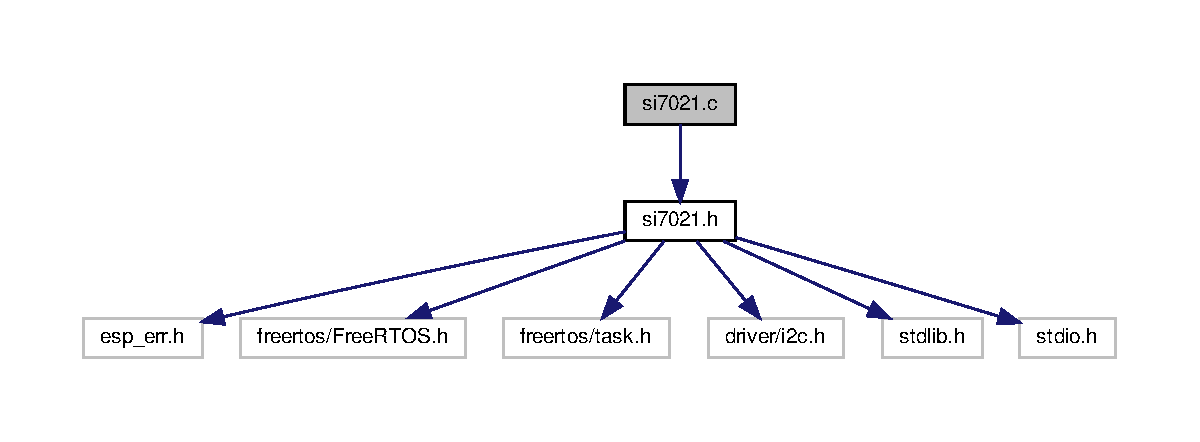
\includegraphics[width=350pt]{si7021_8c__incl}
\end{center}
\end{figure}
\subsection*{Functions}
\begin{DoxyCompactItemize}
\item 
\hyperlink{si7021_8h_aeec681879f00b18fe17bddc989b9582d}{si7021\+\_\+err\+\_\+t} \hyperlink{si7021_8c_a82f9c8e22626638e47729098f8493c1f}{si7021\+\_\+init} (\hyperlink{structsi7021__config__t}{si7021\+\_\+config\+\_\+t} $\ast$config)
\begin{DoxyCompactList}\small\item\em Initialize S\+I7021 sensor. \end{DoxyCompactList}\item 
\hyperlink{si7021_8h_aeec681879f00b18fe17bddc989b9582d}{si7021\+\_\+err\+\_\+t} \hyperlink{si7021_8c_a339f08aa1ed1d74c2c12fd904ea4e28c}{\+\_\+\+\_\+si7021\+\_\+param\+\_\+config} (\hyperlink{structsi7021__config__t}{si7021\+\_\+config\+\_\+t} $\ast$config)
\begin{DoxyCompactList}\small\item\em Configure I2C Parameter for S\+I7021. \end{DoxyCompactList}\item 
\hyperlink{si7021_8h_aeec681879f00b18fe17bddc989b9582d}{si7021\+\_\+err\+\_\+t} \hyperlink{si7021_8c_a814069add0f4e59b5f254732d37637bf}{\+\_\+\+\_\+si7021\+\_\+driver\+\_\+config} (\hyperlink{structsi7021__config__t}{si7021\+\_\+config\+\_\+t} $\ast$config)
\begin{DoxyCompactList}\small\item\em Configure I2C Driver for S\+I7021. \end{DoxyCompactList}\item 
\hyperlink{si7021_8h_aeec681879f00b18fe17bddc989b9582d}{si7021\+\_\+err\+\_\+t} \hyperlink{si7021_8c_a17554408b2bda4f9219d479946e30fbb}{si7021\+\_\+check\+\_\+availability} ()
\begin{DoxyCompactList}\small\item\em Check the availability of sensor. \end{DoxyCompactList}\item 
float \hyperlink{si7021_8c_aac2b7c97826cdeb499ac224a8120fee2}{si7021\+\_\+read\+\_\+temperature} ()
\begin{DoxyCompactList}\small\item\em Read temperature value from sensor. \end{DoxyCompactList}\item 
float \hyperlink{si7021_8c_afebf7dfa4b71f1d0848955edf97a8156}{si7021\+\_\+read\+\_\+humidity} ()
\begin{DoxyCompactList}\small\item\em Read \href{https://en.wikipedia.org/wiki/Relative_humidity}{\tt Relative Humidity} value from sensor. \end{DoxyCompactList}\item 
uint16\+\_\+t \hyperlink{si7021_8c_a57535a0d0725840325a86fd77e609ed2}{\+\_\+\+\_\+si7021\+\_\+read} (uint8\+\_\+t command)
\begin{DoxyCompactList}\small\item\em Get data from sensors by issuing read command and read data return by sensor. \end{DoxyCompactList}\item 
bool \hyperlink{si7021_8c_afee080ad732330932eed4d9d1d93b45f}{\+\_\+\+\_\+is\+\_\+crc\+\_\+valid} (uint16\+\_\+t value, uint8\+\_\+t crc)
\begin{DoxyCompactList}\small\item\em Check data integrity with crc. \end{DoxyCompactList}\item 
uint8\+\_\+t \hyperlink{si7021_8c_abb290c564f829818bb8160cc5a8c93d9}{si7021\+\_\+soft\+\_\+reset} ()
\begin{DoxyCompactList}\small\item\em Reset the sensor. \end{DoxyCompactList}\item 
uint8\+\_\+t \hyperlink{si7021_8c_a91041d121bd0dff34dc9383479286e2d}{\+\_\+\+\_\+si7021\+\_\+read\+\_\+user\+\_\+register} ()
\begin{DoxyCompactList}\small\item\em Read R\+H/T user register 1 from sensor. \end{DoxyCompactList}\item 
uint8\+\_\+t \hyperlink{si7021_8c_a0558cec0e5916d2bc09a51680fa04c2e}{si7021\+\_\+get\+\_\+resolution} ()
\begin{DoxyCompactList}\small\item\em Get current resolution of sensor. \end{DoxyCompactList}\item 
\hyperlink{si7021_8h_aeec681879f00b18fe17bddc989b9582d}{si7021\+\_\+err\+\_\+t} \hyperlink{si7021_8c_a4d97945c1a14dd11da33f3fabacf6b27}{si7021\+\_\+set\+\_\+resolution} (uint8\+\_\+t resolution)
\begin{DoxyCompactList}\small\item\em Set the sensors resolution. \end{DoxyCompactList}\item 
\hyperlink{si7021_8h_aeec681879f00b18fe17bddc989b9582d}{si7021\+\_\+err\+\_\+t} \hyperlink{si7021_8c_ab01f45ffce7fdfa1f150f4b3f15c4e33}{\+\_\+\+\_\+si7021\+\_\+write\+\_\+user\+\_\+register} (uint8\+\_\+t value)
\begin{DoxyCompactList}\small\item\em Write value to R\+H/T user register 1. \end{DoxyCompactList}\item 
uint8\+\_\+t \hyperlink{si7021_8c_a1e1e3955782fa3079544f048d42ad88e}{si7021\+\_\+read\+\_\+firmware\+\_\+rev} ()
\begin{DoxyCompactList}\small\item\em Read sensor firmware revision. \end{DoxyCompactList}\item 
uint8\+\_\+t \hyperlink{si7021_8c_a140788067480f8a462ed2db6a07154d1}{si7021\+\_\+read\+\_\+vdd\+\_\+status} ()
\begin{DoxyCompactList}\small\item\em Check sensors V\+DD. \end{DoxyCompactList}\item 
uint8\+\_\+t \hyperlink{si7021_8c_a6ec069cec3b96b638c8f0426aca309b2}{si7021\+\_\+get\+\_\+heater\+\_\+status} ()
\begin{DoxyCompactList}\small\item\em Check sensors heater status. \end{DoxyCompactList}\item 
uint8\+\_\+t \hyperlink{si7021_8c_ad85d7885ebbb87e1ac1f12b78a6c0af7}{si7021\+\_\+get\+\_\+heater\+\_\+register} ()
\begin{DoxyCompactList}\small\item\em Read heater register. \end{DoxyCompactList}\item 
\hyperlink{si7021_8h_aeec681879f00b18fe17bddc989b9582d}{si7021\+\_\+err\+\_\+t} \hyperlink{si7021_8c_ab4db1385ee975ed53c1b4cb8b2f82da7}{si7021\+\_\+set\+\_\+heater\+\_\+register} (uint8\+\_\+t value)
\begin{DoxyCompactList}\small\item\em Set heater register. \end{DoxyCompactList}\item 
\hyperlink{si7021_8h_aeec681879f00b18fe17bddc989b9582d}{si7021\+\_\+err\+\_\+t} \hyperlink{si7021_8c_a65fe3b1e33bdbebf8df2c8d51bbbf675}{si7021\+\_\+set\+\_\+heater\+\_\+status} (uint8\+\_\+t value)
\begin{DoxyCompactList}\small\item\em Set heater status. \end{DoxyCompactList}\item 
uint64\+\_\+t \hyperlink{si7021_8c_ab0d521e94113c17457f8898e37410009}{get\+\_\+electronic\+\_\+id} ()
\begin{DoxyCompactList}\small\item\em Get sensor electronic id. \end{DoxyCompactList}\end{DoxyCompactItemize}
\subsection*{Variables}
\begin{DoxyCompactItemize}
\item 
\hyperlink{structsi7021__config__t}{si7021\+\_\+config\+\_\+t} \hyperlink{si7021_8c_a7961a32ca6f5fed329358f12119b97b6}{\+\_\+\+\_\+si7021\+\_\+config}
\end{DoxyCompactItemize}


\subsection{Detailed Description}
S\+I7021 Library for E\+S\+P-\/\+I\+DF framework main C file. 

\begin{DoxyAuthor}{Author}
Le Nguyen Hoang Nhan 
\end{DoxyAuthor}
\begin{DoxyDate}{Date}
19 May 2019
\end{DoxyDate}
\begin{DoxySeeAlso}{See also}
\href{https://www.silabs.com/documents/public/data-sheets/Si7021-A20.pdf}{\tt https\+://www.\+silabs.\+com/documents/public/data-\/sheets/\+Si7021-\/\+A20.\+pdf} 
\end{DoxySeeAlso}
\begin{DoxyCopyright}{Copyright}
Copyright (C) 2019 Le Nguyen Hoang Nhan. All rights reserved. 
\end{DoxyCopyright}


\subsection{Function Documentation}
\mbox{\Hypertarget{si7021_8c_afee080ad732330932eed4d9d1d93b45f}\label{si7021_8c_afee080ad732330932eed4d9d1d93b45f}} 
\index{si7021.\+c@{si7021.\+c}!\+\_\+\+\_\+is\+\_\+crc\+\_\+valid@{\+\_\+\+\_\+is\+\_\+crc\+\_\+valid}}
\index{\+\_\+\+\_\+is\+\_\+crc\+\_\+valid@{\+\_\+\+\_\+is\+\_\+crc\+\_\+valid}!si7021.\+c@{si7021.\+c}}
\subsubsection{\texorpdfstring{\+\_\+\+\_\+is\+\_\+crc\+\_\+valid()}{\_\_is\_crc\_valid()}}
{\footnotesize\ttfamily bool \+\_\+\+\_\+is\+\_\+crc\+\_\+valid (\begin{DoxyParamCaption}\item[{uint16\+\_\+t}]{value,  }\item[{uint8\+\_\+t}]{crc }\end{DoxyParamCaption})}



Check data integrity with crc. 


\begin{DoxyParams}{Parameters}
{\em value} & 16bit (uint16\+\_\+t) value that contain data return by sensors. \\
\hline
{\em crc} & 8bit (uint8\+\_\+t) value of crc data \\
\hline
\end{DoxyParams}
\begin{DoxyReturn}{Returns}

\begin{DoxyItemize}
\item boolean value, true if crc value is valid, otherwise false 
\end{DoxyItemize}
\end{DoxyReturn}


Definition at line 142 of file si7021.\+c.



Referenced by \+\_\+\+\_\+si7021\+\_\+read().

\mbox{\Hypertarget{si7021_8c_a814069add0f4e59b5f254732d37637bf}\label{si7021_8c_a814069add0f4e59b5f254732d37637bf}} 
\index{si7021.\+c@{si7021.\+c}!\+\_\+\+\_\+si7021\+\_\+driver\+\_\+config@{\+\_\+\+\_\+si7021\+\_\+driver\+\_\+config}}
\index{\+\_\+\+\_\+si7021\+\_\+driver\+\_\+config@{\+\_\+\+\_\+si7021\+\_\+driver\+\_\+config}!si7021.\+c@{si7021.\+c}}
\subsubsection{\texorpdfstring{\+\_\+\+\_\+si7021\+\_\+driver\+\_\+config()}{\_\_si7021\_driver\_config()}}
{\footnotesize\ttfamily \hyperlink{si7021_8h_aeec681879f00b18fe17bddc989b9582d}{si7021\+\_\+err\+\_\+t} \+\_\+\+\_\+si7021\+\_\+driver\+\_\+config (\begin{DoxyParamCaption}\item[{\hyperlink{structsi7021__config__t}{si7021\+\_\+config\+\_\+t} $\ast$}]{config }\end{DoxyParamCaption})}



Configure I2C Driver for S\+I7021. 

\begin{DoxyNote}{Note}
Internal use only 
\end{DoxyNote}

\begin{DoxyParams}{Parameters}
{\em config} & Forwarded parameter from \hyperlink{si7021_8h_a82f9c8e22626638e47729098f8493c1f}{si7021\+\_\+init}(\hyperlink{structsi7021__config__t}{si7021\+\_\+config\+\_\+t} $\ast$config) \\
\hline
\end{DoxyParams}
\begin{DoxyReturn}{Returns}

\begin{DoxyItemize}
\item \hyperlink{group__SI7021__RT__VALUE_ga04cef12730209bc72277b64111308b42}{S\+I7021\+\_\+\+E\+R\+R\+\_\+\+OK} Success
\item \hyperlink{group__SI7021__RT__VALUE_ga0abfa8d0b3297244d470fcdbce8e39da}{S\+I7021\+\_\+\+E\+R\+R\+\_\+\+C\+O\+N\+F\+IG} Failed to install I2C parameters 
\end{DoxyItemize}
\end{DoxyReturn}


Definition at line 61 of file si7021.\+c.



References S\+I7021\+\_\+\+E\+R\+R\+\_\+\+I\+N\+S\+T\+A\+LL, S\+I7021\+\_\+\+E\+R\+R\+\_\+\+OK, and si7021\+\_\+config\+\_\+t\+::si7021\+\_\+port.



Referenced by si7021\+\_\+init().

\mbox{\Hypertarget{si7021_8c_a339f08aa1ed1d74c2c12fd904ea4e28c}\label{si7021_8c_a339f08aa1ed1d74c2c12fd904ea4e28c}} 
\index{si7021.\+c@{si7021.\+c}!\+\_\+\+\_\+si7021\+\_\+param\+\_\+config@{\+\_\+\+\_\+si7021\+\_\+param\+\_\+config}}
\index{\+\_\+\+\_\+si7021\+\_\+param\+\_\+config@{\+\_\+\+\_\+si7021\+\_\+param\+\_\+config}!si7021.\+c@{si7021.\+c}}
\subsubsection{\texorpdfstring{\+\_\+\+\_\+si7021\+\_\+param\+\_\+config()}{\_\_si7021\_param\_config()}}
{\footnotesize\ttfamily \hyperlink{si7021_8h_aeec681879f00b18fe17bddc989b9582d}{si7021\+\_\+err\+\_\+t} \+\_\+\+\_\+si7021\+\_\+param\+\_\+config (\begin{DoxyParamCaption}\item[{\hyperlink{structsi7021__config__t}{si7021\+\_\+config\+\_\+t} $\ast$}]{config }\end{DoxyParamCaption})}



Configure I2C Parameter for S\+I7021. 

\begin{DoxyNote}{Note}
Internal use only 
\end{DoxyNote}

\begin{DoxyParams}{Parameters}
{\em config} & Forwarded parameter from \hyperlink{si7021_8h_a82f9c8e22626638e47729098f8493c1f}{si7021\+\_\+init}(\hyperlink{structsi7021__config__t}{si7021\+\_\+config\+\_\+t} $\ast$config) \\
\hline
\end{DoxyParams}
\begin{DoxyReturn}{Returns}

\begin{DoxyItemize}
\item \hyperlink{group__SI7021__RT__VALUE_ga04cef12730209bc72277b64111308b42}{S\+I7021\+\_\+\+E\+R\+R\+\_\+\+OK} Success.
\item \hyperlink{group__SI7021__RT__VALUE_ga0abfa8d0b3297244d470fcdbce8e39da}{S\+I7021\+\_\+\+E\+R\+R\+\_\+\+C\+O\+N\+F\+IG} Failed to configure I2C parameter 
\end{DoxyItemize}
\end{DoxyReturn}


Definition at line 50 of file si7021.\+c.



References si7021\+\_\+config\+\_\+t\+::sensors\+\_\+config, S\+I7021\+\_\+\+E\+R\+R\+\_\+\+C\+O\+N\+F\+IG, S\+I7021\+\_\+\+E\+R\+R\+\_\+\+OK, and si7021\+\_\+config\+\_\+t\+::si7021\+\_\+port.



Referenced by si7021\+\_\+init().

\mbox{\Hypertarget{si7021_8c_a57535a0d0725840325a86fd77e609ed2}\label{si7021_8c_a57535a0d0725840325a86fd77e609ed2}} 
\index{si7021.\+c@{si7021.\+c}!\+\_\+\+\_\+si7021\+\_\+read@{\+\_\+\+\_\+si7021\+\_\+read}}
\index{\+\_\+\+\_\+si7021\+\_\+read@{\+\_\+\+\_\+si7021\+\_\+read}!si7021.\+c@{si7021.\+c}}
\subsubsection{\texorpdfstring{\+\_\+\+\_\+si7021\+\_\+read()}{\_\_si7021\_read()}}
{\footnotesize\ttfamily uint16\+\_\+t \+\_\+\+\_\+si7021\+\_\+read (\begin{DoxyParamCaption}\item[{uint8\+\_\+t}]{cmd }\end{DoxyParamCaption})}



Get data from sensors by issuing read command and read data return by sensor. 

\begin{DoxyNote}{Note}
Internal use only 
\end{DoxyNote}

\begin{DoxyParams}{Parameters}
{\em cmd} & Command that will be sent to sensor \\
\hline
\end{DoxyParams}
\begin{DoxyReturn}{Returns}
16bit value (uint16\+\_\+t) contain data from sensors 
\end{DoxyReturn}
\begin{DoxyNote}{Note}
This function will print to console if crc value is invalid 
\end{DoxyNote}


Definition at line 102 of file si7021.\+c.



References \+\_\+\+\_\+is\+\_\+crc\+\_\+valid(), S\+I7021\+\_\+\+A\+D\+DR, and si7021\+\_\+config\+\_\+t\+::si7021\+\_\+port.



Referenced by si7021\+\_\+read\+\_\+humidity(), and si7021\+\_\+read\+\_\+temperature().

Here is the call graph for this function\+:\nopagebreak
\begin{figure}[H]
\begin{center}
\leavevmode
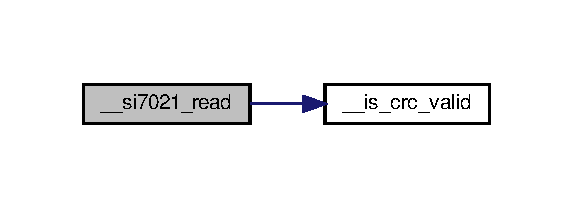
\includegraphics[width=275pt]{si7021_8c_a57535a0d0725840325a86fd77e609ed2_cgraph}
\end{center}
\end{figure}
\mbox{\Hypertarget{si7021_8c_a91041d121bd0dff34dc9383479286e2d}\label{si7021_8c_a91041d121bd0dff34dc9383479286e2d}} 
\index{si7021.\+c@{si7021.\+c}!\+\_\+\+\_\+si7021\+\_\+read\+\_\+user\+\_\+register@{\+\_\+\+\_\+si7021\+\_\+read\+\_\+user\+\_\+register}}
\index{\+\_\+\+\_\+si7021\+\_\+read\+\_\+user\+\_\+register@{\+\_\+\+\_\+si7021\+\_\+read\+\_\+user\+\_\+register}!si7021.\+c@{si7021.\+c}}
\subsubsection{\texorpdfstring{\+\_\+\+\_\+si7021\+\_\+read\+\_\+user\+\_\+register()}{\_\_si7021\_read\_user\_register()}}
{\footnotesize\ttfamily uint8\+\_\+t \+\_\+\+\_\+si7021\+\_\+read\+\_\+user\+\_\+register (\begin{DoxyParamCaption}{ }\end{DoxyParamCaption})}



Read R\+H/T user register 1 from sensor. 

\begin{DoxyNote}{Note}
Internal use only 
\end{DoxyNote}
\begin{DoxyReturn}{Returns}

\begin{DoxyItemize}
\item 8bit (unit8\+\_\+t) value, contain content of user R\+H/T register
\item 0 if failed to read 
\end{DoxyItemize}
\end{DoxyReturn}


Definition at line 193 of file si7021.\+c.



References S\+I7021\+\_\+\+A\+D\+DR, si7021\+\_\+config\+\_\+t\+::si7021\+\_\+port, and S\+I7021\+\_\+\+R\+E\+A\+D\+R\+H\+T\+\_\+\+R\+E\+G\+\_\+\+C\+MD.



Referenced by si7021\+\_\+get\+\_\+heater\+\_\+status(), si7021\+\_\+get\+\_\+resolution(), si7021\+\_\+read\+\_\+vdd\+\_\+status(), si7021\+\_\+set\+\_\+heater\+\_\+status(), and si7021\+\_\+set\+\_\+resolution().

\mbox{\Hypertarget{si7021_8c_ab01f45ffce7fdfa1f150f4b3f15c4e33}\label{si7021_8c_ab01f45ffce7fdfa1f150f4b3f15c4e33}} 
\index{si7021.\+c@{si7021.\+c}!\+\_\+\+\_\+si7021\+\_\+write\+\_\+user\+\_\+register@{\+\_\+\+\_\+si7021\+\_\+write\+\_\+user\+\_\+register}}
\index{\+\_\+\+\_\+si7021\+\_\+write\+\_\+user\+\_\+register@{\+\_\+\+\_\+si7021\+\_\+write\+\_\+user\+\_\+register}!si7021.\+c@{si7021.\+c}}
\subsubsection{\texorpdfstring{\+\_\+\+\_\+si7021\+\_\+write\+\_\+user\+\_\+register()}{\_\_si7021\_write\_user\_register()}}
{\footnotesize\ttfamily \hyperlink{si7021_8h_aeec681879f00b18fe17bddc989b9582d}{si7021\+\_\+err\+\_\+t} \+\_\+\+\_\+si7021\+\_\+write\+\_\+user\+\_\+register (\begin{DoxyParamCaption}\item[{uint8\+\_\+t}]{value }\end{DoxyParamCaption})}



Write value to R\+H/T user register 1. 

\begin{DoxyNote}{Note}
Internal use only 
\end{DoxyNote}

\begin{DoxyParams}{Parameters}
{\em value} & Value to write to register \\
\hline
\end{DoxyParams}
\begin{DoxyReturn}{Returns}

\begin{DoxyItemize}
\item \hyperlink{group__SI7021__RT__VALUE_ga04cef12730209bc72277b64111308b42}{S\+I7021\+\_\+\+E\+R\+R\+\_\+\+OK} Success
\item \hyperlink{group__SI7021__RT__VALUE_gad1c1ac433562f82e632c21f92c0fd4a3}{S\+I7021\+\_\+\+E\+R\+R\+\_\+\+I\+N\+V\+A\+L\+I\+D\+\_\+\+A\+RG} Invalid arguments
\item \hyperlink{group__SI7021__RT__VALUE_ga7cc0cccf705f1f1807d09abc3d1bea14}{S\+I7021\+\_\+\+E\+R\+R\+\_\+\+F\+A\+IL} Failed to write
\item \hyperlink{group__SI7021__RT__VALUE_gadf36521836ea146264b0db90fd02fb45}{S\+I7021\+\_\+\+E\+R\+R\+\_\+\+I\+N\+V\+A\+L\+I\+D\+\_\+\+S\+T\+A\+TE} Sensor is in invalid state
\item \hyperlink{group__SI7021__RT__VALUE_gaf3c553ace8f63aa562e2263c47a1b5ed}{S\+I7021\+\_\+\+E\+R\+R\+\_\+\+T\+I\+M\+E\+O\+UT} Timed out communicating with sensor 
\end{DoxyItemize}
\end{DoxyReturn}


Definition at line 240 of file si7021.\+c.



References S\+I7021\+\_\+\+A\+D\+DR, S\+I7021\+\_\+\+E\+R\+R\+\_\+\+F\+A\+IL, S\+I7021\+\_\+\+E\+R\+R\+\_\+\+I\+N\+V\+A\+L\+I\+D\+\_\+\+A\+RG, S\+I7021\+\_\+\+E\+R\+R\+\_\+\+I\+N\+V\+A\+L\+I\+D\+\_\+\+S\+T\+A\+TE, S\+I7021\+\_\+\+E\+R\+R\+\_\+\+OK, S\+I7021\+\_\+\+E\+R\+R\+\_\+\+T\+I\+M\+E\+O\+UT, si7021\+\_\+config\+\_\+t\+::si7021\+\_\+port, and S\+I7021\+\_\+\+W\+R\+I\+T\+E\+R\+H\+T\+\_\+\+R\+E\+G\+\_\+\+C\+MD.



Referenced by si7021\+\_\+set\+\_\+heater\+\_\+status(), and si7021\+\_\+set\+\_\+resolution().

\mbox{\Hypertarget{si7021_8c_ab0d521e94113c17457f8898e37410009}\label{si7021_8c_ab0d521e94113c17457f8898e37410009}} 
\index{si7021.\+c@{si7021.\+c}!get\+\_\+electronic\+\_\+id@{get\+\_\+electronic\+\_\+id}}
\index{get\+\_\+electronic\+\_\+id@{get\+\_\+electronic\+\_\+id}!si7021.\+c@{si7021.\+c}}
\subsubsection{\texorpdfstring{get\+\_\+electronic\+\_\+id()}{get\_electronic\_id()}}
{\footnotesize\ttfamily uint64\+\_\+t get\+\_\+electronic\+\_\+id (\begin{DoxyParamCaption}{ }\end{DoxyParamCaption})}



Get sensor electronic id. 

\begin{DoxyReturn}{Returns}
64bit (uint64\+\_\+t) value contain sensor electronic id 
\end{DoxyReturn}


Definition at line 370 of file si7021.\+c.



References S\+I7021\+\_\+\+A\+D\+DR, S\+I7021\+\_\+\+I\+D1\+\_\+\+C\+MD, S\+I7021\+\_\+\+I\+D2\+\_\+\+C\+MD, and si7021\+\_\+config\+\_\+t\+::si7021\+\_\+port.

\mbox{\Hypertarget{si7021_8c_a17554408b2bda4f9219d479946e30fbb}\label{si7021_8c_a17554408b2bda4f9219d479946e30fbb}} 
\index{si7021.\+c@{si7021.\+c}!si7021\+\_\+check\+\_\+availability@{si7021\+\_\+check\+\_\+availability}}
\index{si7021\+\_\+check\+\_\+availability@{si7021\+\_\+check\+\_\+availability}!si7021.\+c@{si7021.\+c}}
\subsubsection{\texorpdfstring{si7021\+\_\+check\+\_\+availability()}{si7021\_check\_availability()}}
{\footnotesize\ttfamily \hyperlink{si7021_8h_aeec681879f00b18fe17bddc989b9582d}{si7021\+\_\+err\+\_\+t} si7021\+\_\+check\+\_\+availability (\begin{DoxyParamCaption}{ }\end{DoxyParamCaption})}



Check the availability of sensor. 

\begin{DoxyReturn}{Returns}

\begin{DoxyItemize}
\item \hyperlink{group__SI7021__RT__VALUE_ga04cef12730209bc72277b64111308b42}{S\+I7021\+\_\+\+E\+R\+R\+\_\+\+OK} Sensor detected and available
\item \hyperlink{group__SI7021__RT__VALUE_ga277249c1e2c9ac97e4bec42c79ad4e49}{S\+I7021\+\_\+\+E\+R\+R\+\_\+\+N\+O\+T\+F\+O\+U\+ND} Sensor missing and/or not available 
\end{DoxyItemize}
\end{DoxyReturn}


Definition at line 71 of file si7021.\+c.



References S\+I7021\+\_\+\+A\+D\+DR, S\+I7021\+\_\+\+E\+R\+R\+\_\+\+N\+O\+T\+F\+O\+U\+ND, S\+I7021\+\_\+\+E\+R\+R\+\_\+\+OK, and si7021\+\_\+config\+\_\+t\+::si7021\+\_\+port.



Referenced by si7021\+\_\+init().

\mbox{\Hypertarget{si7021_8c_ad85d7885ebbb87e1ac1f12b78a6c0af7}\label{si7021_8c_ad85d7885ebbb87e1ac1f12b78a6c0af7}} 
\index{si7021.\+c@{si7021.\+c}!si7021\+\_\+get\+\_\+heater\+\_\+register@{si7021\+\_\+get\+\_\+heater\+\_\+register}}
\index{si7021\+\_\+get\+\_\+heater\+\_\+register@{si7021\+\_\+get\+\_\+heater\+\_\+register}!si7021.\+c@{si7021.\+c}}
\subsubsection{\texorpdfstring{si7021\+\_\+get\+\_\+heater\+\_\+register()}{si7021\_get\_heater\_register()}}
{\footnotesize\ttfamily uint8\+\_\+t si7021\+\_\+get\+\_\+heater\+\_\+register (\begin{DoxyParamCaption}{ }\end{DoxyParamCaption})}



Read heater register. 

\begin{DoxyReturn}{Returns}
8bit (uint8\+\_\+t) value contain content of heater register
\begin{DoxyItemize}
\item 0xF\+: 94.\+20mA
\item 0x8\+: 51.\+96mA
\item 0x4\+: 27.\+39mA
\item 0x2\+: 15.\+24mA
\item 0x1\+: 9.\+18mA
\item 0x0\+: 3.\+09mA 
\end{DoxyItemize}
\end{DoxyReturn}


Definition at line 311 of file si7021.\+c.



References S\+I7021\+\_\+\+A\+D\+DR, si7021\+\_\+config\+\_\+t\+::si7021\+\_\+port, and S\+I7021\+\_\+\+R\+E\+A\+D\+H\+E\+A\+T\+E\+R\+\_\+\+R\+E\+G\+\_\+\+C\+MD.

\mbox{\Hypertarget{si7021_8c_a6ec069cec3b96b638c8f0426aca309b2}\label{si7021_8c_a6ec069cec3b96b638c8f0426aca309b2}} 
\index{si7021.\+c@{si7021.\+c}!si7021\+\_\+get\+\_\+heater\+\_\+status@{si7021\+\_\+get\+\_\+heater\+\_\+status}}
\index{si7021\+\_\+get\+\_\+heater\+\_\+status@{si7021\+\_\+get\+\_\+heater\+\_\+status}!si7021.\+c@{si7021.\+c}}
\subsubsection{\texorpdfstring{si7021\+\_\+get\+\_\+heater\+\_\+status()}{si7021\_get\_heater\_status()}}
{\footnotesize\ttfamily uint8\+\_\+t si7021\+\_\+get\+\_\+heater\+\_\+status (\begin{DoxyParamCaption}{ }\end{DoxyParamCaption})}



Check sensors heater status. 

\begin{DoxyReturn}{Returns}
8bit (uint8\+\_\+t) value
\begin{DoxyItemize}
\item \hyperlink{si7021_8h_af209481235e9da082e1447dc34478651}{S\+I7021\+\_\+\+H\+E\+A\+T\+E\+R\+\_\+\+ON} H\+E\+A\+T\+ER is ON
\item \hyperlink{si7021_8h_a7b49e55ef2f682cfe12cd29a09283e68}{S\+I7021\+\_\+\+H\+E\+A\+T\+E\+R\+\_\+\+O\+FF} H\+E\+A\+T\+ER is O\+FF 
\end{DoxyItemize}
\end{DoxyReturn}


Definition at line 304 of file si7021.\+c.



References \+\_\+\+\_\+si7021\+\_\+read\+\_\+user\+\_\+register(), S\+I7021\+\_\+\+H\+E\+A\+T\+E\+R\+\_\+\+O\+FF, and S\+I7021\+\_\+\+H\+E\+A\+T\+E\+R\+\_\+\+ON.

Here is the call graph for this function\+:
\nopagebreak
\begin{figure}[H]
\begin{center}
\leavevmode
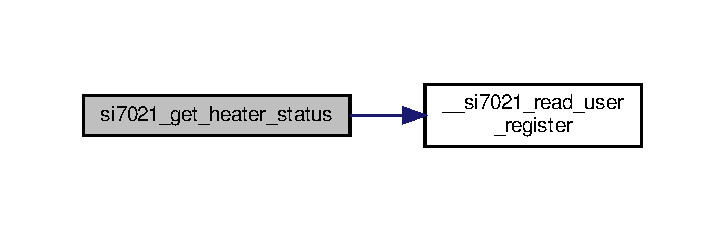
\includegraphics[width=348pt]{si7021_8c_a6ec069cec3b96b638c8f0426aca309b2_cgraph}
\end{center}
\end{figure}
\mbox{\Hypertarget{si7021_8c_a0558cec0e5916d2bc09a51680fa04c2e}\label{si7021_8c_a0558cec0e5916d2bc09a51680fa04c2e}} 
\index{si7021.\+c@{si7021.\+c}!si7021\+\_\+get\+\_\+resolution@{si7021\+\_\+get\+\_\+resolution}}
\index{si7021\+\_\+get\+\_\+resolution@{si7021\+\_\+get\+\_\+resolution}!si7021.\+c@{si7021.\+c}}
\subsubsection{\texorpdfstring{si7021\+\_\+get\+\_\+resolution()}{si7021\_get\_resolution()}}
{\footnotesize\ttfamily uint8\+\_\+t si7021\+\_\+get\+\_\+resolution (\begin{DoxyParamCaption}{ }\end{DoxyParamCaption})}



Get current resolution of sensor. 

\begin{DoxyReturn}{Returns}

\begin{DoxyItemize}
\item 0x00\+: 12bit RH resolution, 14bit temperature resolution
\item 0x01\+: 8bit RH resolution, 12bit temperature resolution
\item 0x80\+: 10bit RH resolution, 13bit temperature resolution
\item 0x81\+: 11bit RH resolution, 11bit temperature resolution 
\end{DoxyItemize}
\end{DoxyReturn}


Definition at line 221 of file si7021.\+c.



References \+\_\+\+\_\+si7021\+\_\+read\+\_\+user\+\_\+register().

Here is the call graph for this function\+:
\nopagebreak
\begin{figure}[H]
\begin{center}
\leavevmode
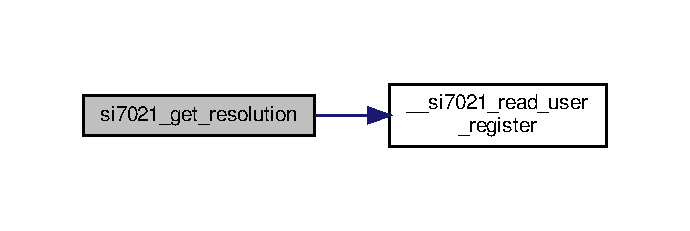
\includegraphics[width=331pt]{si7021_8c_a0558cec0e5916d2bc09a51680fa04c2e_cgraph}
\end{center}
\end{figure}
\mbox{\Hypertarget{si7021_8c_a82f9c8e22626638e47729098f8493c1f}\label{si7021_8c_a82f9c8e22626638e47729098f8493c1f}} 
\index{si7021.\+c@{si7021.\+c}!si7021\+\_\+init@{si7021\+\_\+init}}
\index{si7021\+\_\+init@{si7021\+\_\+init}!si7021.\+c@{si7021.\+c}}
\subsubsection{\texorpdfstring{si7021\+\_\+init()}{si7021\_init()}}
{\footnotesize\ttfamily \hyperlink{si7021_8h_aeec681879f00b18fe17bddc989b9582d}{si7021\+\_\+err\+\_\+t} si7021\+\_\+init (\begin{DoxyParamCaption}\item[{\hyperlink{structsi7021__config__t}{si7021\+\_\+config\+\_\+t} $\ast$}]{config }\end{DoxyParamCaption})}



Initialize S\+I7021 sensor. 


\begin{DoxyParams}{Parameters}
{\em config} & \hyperlink{structsi7021__config__t}{si7021\+\_\+config\+\_\+t} struct that contain sensors information and configuration \\
\hline
\end{DoxyParams}
\begin{DoxyReturn}{Returns}

\begin{DoxyItemize}
\item \hyperlink{group__SI7021__RT__VALUE_ga04cef12730209bc72277b64111308b42}{S\+I7021\+\_\+\+E\+R\+R\+\_\+\+OK} Success.
\item \hyperlink{group__SI7021__RT__VALUE_ga0abfa8d0b3297244d470fcdbce8e39da}{S\+I7021\+\_\+\+E\+R\+R\+\_\+\+C\+O\+N\+F\+IG} Failed to configure I2C parameter, forwarded return from \hyperlink{si7021_8h_a339f08aa1ed1d74c2c12fd904ea4e28c}{\+\_\+\+\_\+si7021\+\_\+param\+\_\+config}(\hyperlink{structsi7021__config__t}{si7021\+\_\+config\+\_\+t} $\ast$config)
\item \hyperlink{group__SI7021__RT__VALUE_ga1a536c4aff63acd66547e006b587841b}{S\+I7021\+\_\+\+E\+R\+R\+\_\+\+I\+N\+S\+T\+A\+LL} Failed to configure I2C Driver, forwarded return from \hyperlink{si7021_8h_a814069add0f4e59b5f254732d37637bf}{\+\_\+\+\_\+si7021\+\_\+driver\+\_\+config}(\hyperlink{structsi7021__config__t}{si7021\+\_\+config\+\_\+t} $\ast$config)
\item \hyperlink{group__SI7021__RT__VALUE_ga277249c1e2c9ac97e4bec42c79ad4e49}{S\+I7021\+\_\+\+E\+R\+R\+\_\+\+N\+O\+T\+F\+O\+U\+ND} Sensor missing and/or not available, forwarded return from \hyperlink{si7021_8h_a17554408b2bda4f9219d479946e30fbb}{si7021\+\_\+check\+\_\+availability()} 
\end{DoxyItemize}
\end{DoxyReturn}


Definition at line 34 of file si7021.\+c.



References \+\_\+\+\_\+si7021\+\_\+driver\+\_\+config(), \+\_\+\+\_\+si7021\+\_\+param\+\_\+config(), si7021\+\_\+check\+\_\+availability(), and S\+I7021\+\_\+\+E\+R\+R\+\_\+\+OK.

Here is the call graph for this function\+:
\nopagebreak
\begin{figure}[H]
\begin{center}
\leavevmode
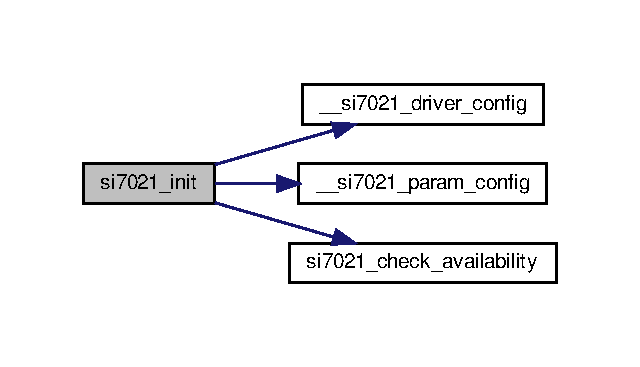
\includegraphics[width=307pt]{si7021_8c_a82f9c8e22626638e47729098f8493c1f_cgraph}
\end{center}
\end{figure}
\mbox{\Hypertarget{si7021_8c_a1e1e3955782fa3079544f048d42ad88e}\label{si7021_8c_a1e1e3955782fa3079544f048d42ad88e}} 
\index{si7021.\+c@{si7021.\+c}!si7021\+\_\+read\+\_\+firmware\+\_\+rev@{si7021\+\_\+read\+\_\+firmware\+\_\+rev}}
\index{si7021\+\_\+read\+\_\+firmware\+\_\+rev@{si7021\+\_\+read\+\_\+firmware\+\_\+rev}!si7021.\+c@{si7021.\+c}}
\subsubsection{\texorpdfstring{si7021\+\_\+read\+\_\+firmware\+\_\+rev()}{si7021\_read\_firmware\_rev()}}
{\footnotesize\ttfamily uint8\+\_\+t si7021\+\_\+read\+\_\+firmware\+\_\+rev (\begin{DoxyParamCaption}{ }\end{DoxyParamCaption})}



Read sensor firmware revision. 

\begin{DoxyReturn}{Returns}
8bit (uint8\+\_\+t) value contain sensor firmware revision
\begin{DoxyItemize}
\item 0x\+FF\+: Firmware version 1.\+0
\item 0x20\+: Firmware version 2.\+0 
\end{DoxyItemize}
\end{DoxyReturn}


Definition at line 269 of file si7021.\+c.



References S\+I7021\+\_\+\+A\+D\+DR, S\+I7021\+\_\+\+F\+I\+R\+M\+V\+E\+R\+S\+\_\+\+C\+MD, and si7021\+\_\+config\+\_\+t\+::si7021\+\_\+port.

\mbox{\Hypertarget{si7021_8c_afebf7dfa4b71f1d0848955edf97a8156}\label{si7021_8c_afebf7dfa4b71f1d0848955edf97a8156}} 
\index{si7021.\+c@{si7021.\+c}!si7021\+\_\+read\+\_\+humidity@{si7021\+\_\+read\+\_\+humidity}}
\index{si7021\+\_\+read\+\_\+humidity@{si7021\+\_\+read\+\_\+humidity}!si7021.\+c@{si7021.\+c}}
\subsubsection{\texorpdfstring{si7021\+\_\+read\+\_\+humidity()}{si7021\_read\_humidity()}}
{\footnotesize\ttfamily float si7021\+\_\+read\+\_\+humidity (\begin{DoxyParamCaption}{ }\end{DoxyParamCaption})}



Read \href{https://en.wikipedia.org/wiki/Relative_humidity}{\tt Relative Humidity} value from sensor. 

\begin{DoxyReturn}{Returns}
float value, \href{https://en.wikipedia.org/wiki/Relative_humidity}{\tt Relative Humidity} in percentage 
\end{DoxyReturn}


Definition at line 94 of file si7021.\+c.



References \+\_\+\+\_\+si7021\+\_\+read(), and S\+I7021\+\_\+\+M\+E\+A\+S\+R\+H\+\_\+\+N\+O\+H\+O\+L\+D\+\_\+\+C\+MD.

Here is the call graph for this function\+:
\nopagebreak
\begin{figure}[H]
\begin{center}
\leavevmode
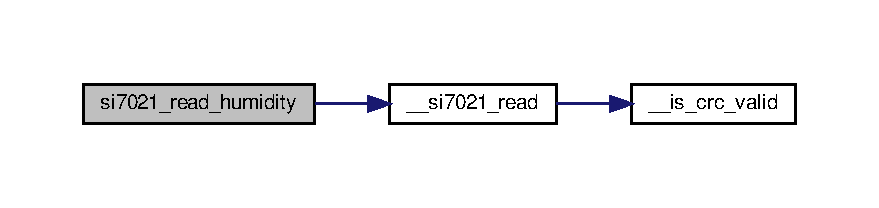
\includegraphics[width=350pt]{si7021_8c_afebf7dfa4b71f1d0848955edf97a8156_cgraph}
\end{center}
\end{figure}
\mbox{\Hypertarget{si7021_8c_aac2b7c97826cdeb499ac224a8120fee2}\label{si7021_8c_aac2b7c97826cdeb499ac224a8120fee2}} 
\index{si7021.\+c@{si7021.\+c}!si7021\+\_\+read\+\_\+temperature@{si7021\+\_\+read\+\_\+temperature}}
\index{si7021\+\_\+read\+\_\+temperature@{si7021\+\_\+read\+\_\+temperature}!si7021.\+c@{si7021.\+c}}
\subsubsection{\texorpdfstring{si7021\+\_\+read\+\_\+temperature()}{si7021\_read\_temperature()}}
{\footnotesize\ttfamily float si7021\+\_\+read\+\_\+temperature (\begin{DoxyParamCaption}{ }\end{DoxyParamCaption})}



Read temperature value from sensor. 

\begin{DoxyReturn}{Returns}
float value, temperature in \href{https://en.wikipedia.org/wiki/Celsius}{\tt Celsius} 
\end{DoxyReturn}


Definition at line 86 of file si7021.\+c.



References \+\_\+\+\_\+si7021\+\_\+read(), and S\+I7021\+\_\+\+M\+E\+A\+S\+T\+E\+M\+P\+\_\+\+N\+O\+H\+O\+L\+D\+\_\+\+C\+MD.

Here is the call graph for this function\+:
\nopagebreak
\begin{figure}[H]
\begin{center}
\leavevmode
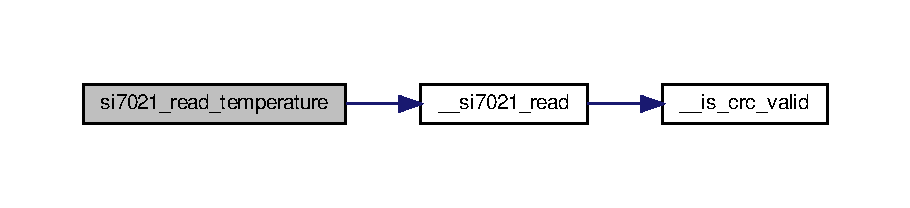
\includegraphics[width=350pt]{si7021_8c_aac2b7c97826cdeb499ac224a8120fee2_cgraph}
\end{center}
\end{figure}
\mbox{\Hypertarget{si7021_8c_a140788067480f8a462ed2db6a07154d1}\label{si7021_8c_a140788067480f8a462ed2db6a07154d1}} 
\index{si7021.\+c@{si7021.\+c}!si7021\+\_\+read\+\_\+vdd\+\_\+status@{si7021\+\_\+read\+\_\+vdd\+\_\+status}}
\index{si7021\+\_\+read\+\_\+vdd\+\_\+status@{si7021\+\_\+read\+\_\+vdd\+\_\+status}!si7021.\+c@{si7021.\+c}}
\subsubsection{\texorpdfstring{si7021\+\_\+read\+\_\+vdd\+\_\+status()}{si7021\_read\_vdd\_status()}}
{\footnotesize\ttfamily uint8\+\_\+t si7021\+\_\+read\+\_\+vdd\+\_\+status (\begin{DoxyParamCaption}{ }\end{DoxyParamCaption})}



Check sensors V\+DD. 

\begin{DoxyReturn}{Returns}
8bit (uint8\+\_\+t) value
\begin{DoxyItemize}
\item \hyperlink{si7021_8h_ac7934e73c20c5721d2781bf20cdb3b3c}{S\+I7021\+\_\+\+V\+D\+D\+\_\+\+OK} V\+DD is OK
\item \hyperlink{si7021_8h_ac3635b86980e04705efb3d2b87aeafe7}{S\+I7021\+\_\+\+V\+D\+D\+\_\+\+L\+OW} V\+DD is L\+OW 
\end{DoxyItemize}
\end{DoxyReturn}
\begin{DoxyNote}{Note}
Consider changing power supply when V\+DD is L\+OW, sensors may not work correctly 
\end{DoxyNote}


Definition at line 297 of file si7021.\+c.



References \+\_\+\+\_\+si7021\+\_\+read\+\_\+user\+\_\+register(), S\+I7021\+\_\+\+V\+D\+D\+\_\+\+L\+OW, and S\+I7021\+\_\+\+V\+D\+D\+\_\+\+OK.

Here is the call graph for this function\+:
\nopagebreak
\begin{figure}[H]
\begin{center}
\leavevmode
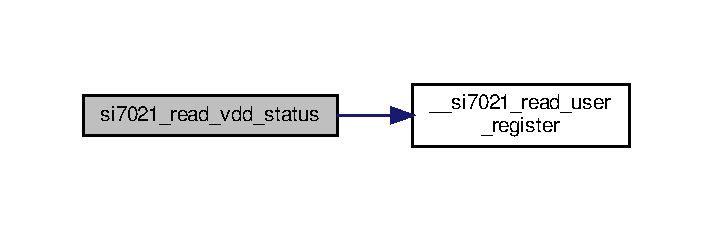
\includegraphics[width=342pt]{si7021_8c_a140788067480f8a462ed2db6a07154d1_cgraph}
\end{center}
\end{figure}
\mbox{\Hypertarget{si7021_8c_ab4db1385ee975ed53c1b4cb8b2f82da7}\label{si7021_8c_ab4db1385ee975ed53c1b4cb8b2f82da7}} 
\index{si7021.\+c@{si7021.\+c}!si7021\+\_\+set\+\_\+heater\+\_\+register@{si7021\+\_\+set\+\_\+heater\+\_\+register}}
\index{si7021\+\_\+set\+\_\+heater\+\_\+register@{si7021\+\_\+set\+\_\+heater\+\_\+register}!si7021.\+c@{si7021.\+c}}
\subsubsection{\texorpdfstring{si7021\+\_\+set\+\_\+heater\+\_\+register()}{si7021\_set\_heater\_register()}}
{\footnotesize\ttfamily \hyperlink{si7021_8h_aeec681879f00b18fe17bddc989b9582d}{si7021\+\_\+err\+\_\+t} si7021\+\_\+set\+\_\+heater\+\_\+register (\begin{DoxyParamCaption}\item[{uint8\+\_\+t}]{value }\end{DoxyParamCaption})}



Set heater register. 


\begin{DoxyParams}{Parameters}
{\em value} & 8bit (uint8\+\_\+t) value that will be written to heater register
\begin{DoxyItemize}
\item 0xF\+: 94.\+20mA
\item 0x8\+: 51.\+96mA
\item 0x4\+: 27.\+39mA
\item 0x2\+: 15.\+24mA
\item 0x1\+: 9.\+18mA
\item 0x0\+: 3.\+09mA 
\end{DoxyItemize}\\
\hline
\end{DoxyParams}


Definition at line 338 of file si7021.\+c.



References S\+I7021\+\_\+\+A\+D\+DR, S\+I7021\+\_\+\+E\+R\+R\+\_\+\+F\+A\+IL, S\+I7021\+\_\+\+E\+R\+R\+\_\+\+I\+N\+V\+A\+L\+I\+D\+\_\+\+A\+RG, S\+I7021\+\_\+\+E\+R\+R\+\_\+\+I\+N\+V\+A\+L\+I\+D\+\_\+\+S\+T\+A\+TE, S\+I7021\+\_\+\+E\+R\+R\+\_\+\+OK, S\+I7021\+\_\+\+E\+R\+R\+\_\+\+T\+I\+M\+E\+O\+UT, si7021\+\_\+config\+\_\+t\+::si7021\+\_\+port, and S\+I7021\+\_\+\+W\+R\+I\+T\+E\+H\+E\+A\+T\+E\+R\+\_\+\+R\+E\+G\+\_\+\+C\+MD.

\mbox{\Hypertarget{si7021_8c_a65fe3b1e33bdbebf8df2c8d51bbbf675}\label{si7021_8c_a65fe3b1e33bdbebf8df2c8d51bbbf675}} 
\index{si7021.\+c@{si7021.\+c}!si7021\+\_\+set\+\_\+heater\+\_\+status@{si7021\+\_\+set\+\_\+heater\+\_\+status}}
\index{si7021\+\_\+set\+\_\+heater\+\_\+status@{si7021\+\_\+set\+\_\+heater\+\_\+status}!si7021.\+c@{si7021.\+c}}
\subsubsection{\texorpdfstring{si7021\+\_\+set\+\_\+heater\+\_\+status()}{si7021\_set\_heater\_status()}}
{\footnotesize\ttfamily \hyperlink{si7021_8h_aeec681879f00b18fe17bddc989b9582d}{si7021\+\_\+err\+\_\+t} si7021\+\_\+set\+\_\+heater\+\_\+status (\begin{DoxyParamCaption}\item[{uint8\+\_\+t}]{value }\end{DoxyParamCaption})}



Set heater status. 


\begin{DoxyParams}{Parameters}
{\em value} & Heater status will be set to this
\begin{DoxyItemize}
\item \hyperlink{si7021_8h_af209481235e9da082e1447dc34478651}{S\+I7021\+\_\+\+H\+E\+A\+T\+E\+R\+\_\+\+ON}\+: H\+E\+A\+T\+ER will be turn on
\item \hyperlink{si7021_8h_a7b49e55ef2f682cfe12cd29a09283e68}{S\+I7021\+\_\+\+H\+E\+A\+T\+E\+R\+\_\+\+O\+FF}\+: H\+E\+A\+T\+ER will be turn off 
\end{DoxyItemize}\\
\hline
\end{DoxyParams}


Definition at line 361 of file si7021.\+c.



References \+\_\+\+\_\+si7021\+\_\+read\+\_\+user\+\_\+register(), \+\_\+\+\_\+si7021\+\_\+write\+\_\+user\+\_\+register(), S\+I7021\+\_\+\+H\+E\+A\+T\+E\+R\+\_\+\+O\+FF, and S\+I7021\+\_\+\+H\+E\+A\+T\+E\+R\+\_\+\+ON.

Here is the call graph for this function\+:
\nopagebreak
\begin{figure}[H]
\begin{center}
\leavevmode
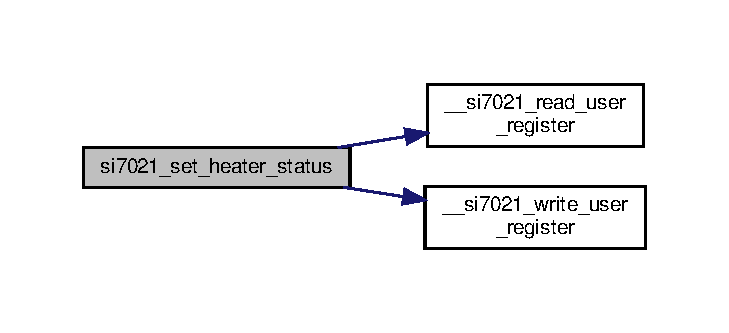
\includegraphics[width=350pt]{si7021_8c_a65fe3b1e33bdbebf8df2c8d51bbbf675_cgraph}
\end{center}
\end{figure}
\mbox{\Hypertarget{si7021_8c_a4d97945c1a14dd11da33f3fabacf6b27}\label{si7021_8c_a4d97945c1a14dd11da33f3fabacf6b27}} 
\index{si7021.\+c@{si7021.\+c}!si7021\+\_\+set\+\_\+resolution@{si7021\+\_\+set\+\_\+resolution}}
\index{si7021\+\_\+set\+\_\+resolution@{si7021\+\_\+set\+\_\+resolution}!si7021.\+c@{si7021.\+c}}
\subsubsection{\texorpdfstring{si7021\+\_\+set\+\_\+resolution()}{si7021\_set\_resolution()}}
{\footnotesize\ttfamily \hyperlink{si7021_8h_aeec681879f00b18fe17bddc989b9582d}{si7021\+\_\+err\+\_\+t} si7021\+\_\+set\+\_\+resolution (\begin{DoxyParamCaption}\item[{uint8\+\_\+t}]{resolution }\end{DoxyParamCaption})}



Set the sensors resolution. 


\begin{DoxyParams}{Parameters}
{\em resolution} & The resolution will be set \\
\hline
\end{DoxyParams}
\begin{DoxyReturn}{Returns}

\begin{DoxyItemize}
\item \hyperlink{group__SI7021__RT__VALUE_ga04cef12730209bc72277b64111308b42}{S\+I7021\+\_\+\+E\+R\+R\+\_\+\+OK} Success
\item \hyperlink{group__SI7021__RT__VALUE_gad1c1ac433562f82e632c21f92c0fd4a3}{S\+I7021\+\_\+\+E\+R\+R\+\_\+\+I\+N\+V\+A\+L\+I\+D\+\_\+\+A\+RG} Invalid arguments
\item \hyperlink{group__SI7021__RT__VALUE_ga7cc0cccf705f1f1807d09abc3d1bea14}{S\+I7021\+\_\+\+E\+R\+R\+\_\+\+F\+A\+IL} Failed to write
\item \hyperlink{group__SI7021__RT__VALUE_gadf36521836ea146264b0db90fd02fb45}{S\+I7021\+\_\+\+E\+R\+R\+\_\+\+I\+N\+V\+A\+L\+I\+D\+\_\+\+S\+T\+A\+TE} Sensor is in invalid state
\item \hyperlink{group__SI7021__RT__VALUE_gaf3c553ace8f63aa562e2263c47a1b5ed}{S\+I7021\+\_\+\+E\+R\+R\+\_\+\+T\+I\+M\+E\+O\+UT} Timed out communicating with sensor 
\end{DoxyItemize}
\end{DoxyReturn}


Definition at line 225 of file si7021.\+c.



References \+\_\+\+\_\+si7021\+\_\+read\+\_\+user\+\_\+register(), and \+\_\+\+\_\+si7021\+\_\+write\+\_\+user\+\_\+register().

Here is the call graph for this function\+:
\nopagebreak
\begin{figure}[H]
\begin{center}
\leavevmode
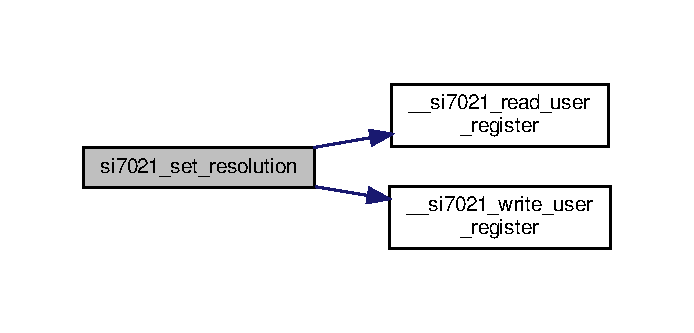
\includegraphics[width=333pt]{si7021_8c_a4d97945c1a14dd11da33f3fabacf6b27_cgraph}
\end{center}
\end{figure}
\mbox{\Hypertarget{si7021_8c_abb290c564f829818bb8160cc5a8c93d9}\label{si7021_8c_abb290c564f829818bb8160cc5a8c93d9}} 
\index{si7021.\+c@{si7021.\+c}!si7021\+\_\+soft\+\_\+reset@{si7021\+\_\+soft\+\_\+reset}}
\index{si7021\+\_\+soft\+\_\+reset@{si7021\+\_\+soft\+\_\+reset}!si7021.\+c@{si7021.\+c}}
\subsubsection{\texorpdfstring{si7021\+\_\+soft\+\_\+reset()}{si7021\_soft\_reset()}}
{\footnotesize\ttfamily uint8\+\_\+t si7021\+\_\+soft\+\_\+reset (\begin{DoxyParamCaption}{ }\end{DoxyParamCaption})}



Reset the sensor. 

\begin{DoxyNote}{Note}
Reset will erase all setting, register... 
\end{DoxyNote}
\begin{DoxyReturn}{Returns}

\begin{DoxyItemize}
\item \hyperlink{group__SI7021__RT__VALUE_ga04cef12730209bc72277b64111308b42}{S\+I7021\+\_\+\+E\+R\+R\+\_\+\+OK} Success
\item \hyperlink{group__SI7021__RT__VALUE_gaf3c553ace8f63aa562e2263c47a1b5ed}{S\+I7021\+\_\+\+E\+R\+R\+\_\+\+T\+I\+M\+E\+O\+UT} Timed out communicating with sensor
\item \hyperlink{group__SI7021__RT__VALUE_gadf36521836ea146264b0db90fd02fb45}{S\+I7021\+\_\+\+E\+R\+R\+\_\+\+I\+N\+V\+A\+L\+I\+D\+\_\+\+S\+T\+A\+TE} Sensor is in invalid state
\item \hyperlink{group__SI7021__RT__VALUE_ga7cc0cccf705f1f1807d09abc3d1bea14}{S\+I7021\+\_\+\+E\+R\+R\+\_\+\+F\+A\+IL} Failed
\item \hyperlink{group__SI7021__RT__VALUE_gad1c1ac433562f82e632c21f92c0fd4a3}{S\+I7021\+\_\+\+E\+R\+R\+\_\+\+I\+N\+V\+A\+L\+I\+D\+\_\+\+A\+RG} Invalid arguments 
\end{DoxyItemize}
\end{DoxyReturn}


Definition at line 167 of file si7021.\+c.



References S\+I7021\+\_\+\+A\+D\+DR, S\+I7021\+\_\+\+E\+R\+R\+\_\+\+F\+A\+IL, S\+I7021\+\_\+\+E\+R\+R\+\_\+\+I\+N\+V\+A\+L\+I\+D\+\_\+\+A\+RG, S\+I7021\+\_\+\+E\+R\+R\+\_\+\+I\+N\+V\+A\+L\+I\+D\+\_\+\+S\+T\+A\+TE, S\+I7021\+\_\+\+E\+R\+R\+\_\+\+OK, S\+I7021\+\_\+\+E\+R\+R\+\_\+\+T\+I\+M\+E\+O\+UT, si7021\+\_\+config\+\_\+t\+::si7021\+\_\+port, and S\+I7021\+\_\+\+S\+O\+F\+T\+\_\+\+R\+E\+S\+E\+T\+\_\+\+C\+MD.



\subsection{Variable Documentation}
\mbox{\Hypertarget{si7021_8c_a7961a32ca6f5fed329358f12119b97b6}\label{si7021_8c_a7961a32ca6f5fed329358f12119b97b6}} 
\index{si7021.\+c@{si7021.\+c}!\+\_\+\+\_\+si7021\+\_\+config@{\+\_\+\+\_\+si7021\+\_\+config}}
\index{\+\_\+\+\_\+si7021\+\_\+config@{\+\_\+\+\_\+si7021\+\_\+config}!si7021.\+c@{si7021.\+c}}
\subsubsection{\texorpdfstring{\+\_\+\+\_\+si7021\+\_\+config}{\_\_si7021\_config}}
{\footnotesize\ttfamily \hyperlink{structsi7021__config__t}{si7021\+\_\+config\+\_\+t} \+\_\+\+\_\+si7021\+\_\+config}

{\bfseries Initial value\+:}
\begin{DoxyCode}
= \{ .sensors\_config = \{ .mode = I2C\_MODE\_MASTER,
        .sda\_io\_num = GPIO\_NUM\_22, .scl\_io\_num = GPIO\_NUM\_23, .sda\_pullup\_en =
                GPIO\_PULLUP\_ENABLE, .scl\_pullup\_en = GPIO\_PULLUP\_ENABLE,
        .master = \{ .clk\_speed = 400000 \}, \}, .si7021\_port = I2C\_NUM\_0 \}
\end{DoxyCode}


Definition at line 29 of file si7021.\+c.


%--- End generated contents ---

% Index
\backmatter
\newpage
\phantomsection
\clearemptydoublepage
\addcontentsline{toc}{chapter}{Index}
\printindex

\end{document}
